\documentclass[12pt,a4paper]{report}
\usepackage[utf8]{inputenc}
\usepackage{graphicx}
\usepackage{hyperref}
\usepackage{listings}
\usepackage{amsmath}
\usepackage{booktabs}
\usepackage{tikz}
\usetikzlibrary{arrows.meta,positioning,shapes.geometric,fit,backgrounds,calc}
\usepackage{pifont}
\newcommand{\cmark}{\ding{51}}%
\newcommand{\xmark}{\ding{55}}%
\usepackage[backend=biber,style=numeric]{biblatex}
\addbibresource{references.bib}

\lstset{
  basicstyle=\ttfamily\small,
  breaklines=true,
  frame=single,
  numbers=left,
  numberstyle=\tiny,
  tabsize=4,
  captionpos=b,
  xleftmargin=2em,
  framexleftmargin=1.5em
}

\title{Documentation-Driven Testing (DDT): A Paradigm for Automated API Quality Assurance in the GitOps Era}
\author{Petros Evangelos Triantafyllis}
\date{2026}

\begin{document}

\maketitle
\tableofcontents

\chapter{Introduction}
\label{ch:introduction}

Modern software systems are built on APIs. They connect microservices, power mobile applications, expose business logic to partners, and increasingly serve as the interface through which autonomous agents interact with the world. Yet the quality assurance practices around these interfaces remain stubbornly manual, disconnected from the declarative pipelines that deploy the very services they test.

This thesis introduces Specification-Driven Testing (SDT)\footnote{An earlier formulation of this work used the name \textit{Documentation-Driven Testing} (DDT); the name \textit{Specification-Driven Testing} is adopted here as more precise, reflecting that the framework operates on a formal API specification (OpenAPI), not on documentation in general.}\textsuperscript{,}\footnote{Throughout the thesis, ``API'' refers specifically to \emph{HTTP-based RESTful APIs} described by the OpenAPI specification (versions 3.0.x and 3.1.0), with limited treatment of Swagger 2.0 via the conversion adapter discussed in Chapter~\ref{ch:architecture}. The framework's axioms are stated at a level of generality that admits extension to other API styles---GraphQL introspection schemas, gRPC service definitions, AsyncAPI for event-driven systems---but those extensions are scoped as future work (Chapter~\ref{ch:conclusion}). Where the text uses ``API'' without qualification, the RESTful + OpenAPI scope is implied.}, a conceptual framework that treats the API specification not merely as documentation, but as the single source of truth from which validation rules, test cases, and quality gates are derived automatically. We present the theoretical foundations of SDT---three axioms grounding nine validation principles---together with an open-source implementation called DriveBy, a declarative Crossplane custom resource (XSDLC) that realises SDT quality gates inside GitOps delivery pipelines, and an empirical evaluation demonstrating its effectiveness across both controlled and large-scale settings. We position SDT explicitly as a conceptual framework---a strong theoretical core for a future formal methodology---rather than as a complete software-testing methodology in its own right; the elements that would be required to elevate it to a full methodology (test derivation procedure, execution and failure semantics, lifecycle governance) are identified as future work in Chapter~\ref{ch:conclusion}.

% ============================================================================
\section{The Cost of Manual Operations}
\label{sec:cost-manual}
% ============================================================================

\subsection{The Talent Drain}
\label{subsec:talent-drain}

Engineering talent is the scarcest resource in software organizations: the 2024 Stack Overflow Developer Survey reports that demand for software engineers continues to outpace supply~\cite{stackoverflow-survey}. Yet a remarkable share of their time goes not to building software but to verifying it by hand; the Postman State of the API Report confirms that manual testing remains the dominant API quality assurance practice~\cite{postman-state-of-api}.

The consequences compound. Forsgren, Humble, and Kim demonstrate that high-performing teams distinguish themselves through automated testing, deployment, and feedback loops, and that organizations failing to automate their quality gates systematically underperform on deployment frequency, lead time, change failure rate, and mean time to recovery~\cite{accelerate}. The question is not whether to automate API quality assurance, but how.

\subsection{Documentation Drift as a Systemic Failure}
\label{subsec:doc-drift}

We define \textit{documentation drift} as the progressive divergence between an API's specification and its actual implementation. Drift is not a one-time event but a continuous process: each deployment that modifies behavior without updating the specification widens the gap. Over time, the specification becomes a historical artifact---accurate at some past commit, unreliable at the current one.

The SmartBear State of API Report identifies documentation quality as the single most important factor in API adoption, yet consistently finds that a majority of API specifications are incomplete, outdated, or both~\cite{smartbear-api-report}. In most organizations, specification updates are a manual after-the-fact step enforced by nothing stronger than code review conventions; when deadlines compress, documentation is the first casualty.

Drift is not laziness but a systemic failure rooted in the separation of two artifacts---the specification and the implementation---that should be governed by a single source of truth. If validation derived from a complete specification ran on every change, drift would be detected at the point of introduction rather than discovered by a frustrated consumer weeks later.

So, what if the documentation itself could be the testing infrastructure?

% ============================================================================
\section{The Shift Toward Declarative Everything}
\label{sec:declarative-shift}
% ============================================================================

\subsection{GitOps and the Declarative Promise}
\label{subsec:gitops}

The past decade witnessed a fundamental shift in how software systems are operated. GitOps, formalized by the CNCF OpenGitOps working group, establishes four principles: declarative desired state, versioned and immutable storage, automated application of state, and continuous reconciliation~\cite{opengitops}. Tools like Argo~CD~\cite{argocd} implement these principles for Kubernetes: an operator does not \textit{do} things to a cluster but \textit{declares} what it should look like, and a reconciliation loop makes it so.

Yet API quality assurance has not followed. Deployments and infrastructure provisioning are declarative, but the validation of the APIs those systems expose remains imperative: teams write tests by hand, run them in ad-hoc pipelines, and interpret results manually~\cite{postman-state-of-api}. Declarative systems are tested with imperative processes.

\subsection{Cloud-Native Infrastructure as Code}
\label{subsec:cloud-native-iac}

The declarative paradigm extends beyond application deployment. Terraform~\cite{terraform} pioneered infrastructure-as-code; Crossplane~\cite{crossplane} turns the Kubernetes API server into a universal control plane that provisions databases, message queues, DNS records, and entire cloud environments through declarative manifests. The Cloud Native Computing Foundation's annual survey reports accelerating adoption of this model~\cite{cncf-survey}, whose philosophy is consistent: if you can describe it, you can automate it; if you can automate it, you can reconcile it; if you can reconcile it, drift disappears.

This philosophy has transformed infrastructure and deployment but not yet API quality assurance. The gap is not technological---OpenAPI specifications already describe APIs declaratively---but methodological: no widely adopted framework treats the specification as the source from which validation is derived, executed, and reconciled automatically.

\subsection{The Agentic Development Frontier}
\label{subsec:agentic-dev}

A parallel development accelerates the urgency. AI-assisted software engineering tools---from code completion systems like GitHub Copilot~\cite{github-copilot-research} to autonomous agents capable of executing multi-step development workflows---are reshaping how software is built. These tools depend on structured, machine-readable inputs. An agent cannot interpret a Confluence page or parse a Slack thread; it requires formal specifications with well-defined semantics. This observation yields an explicit requirement for any quality-assurance methodology intended to operate in this setting: it must produce structured, specification-grounded quality signals that agents can consume and act upon without human interpretation.

SDT fulfils this requirement: its validation results are structured, machine-readable quality signals tied directly to the specification, which a CI pipeline can gate on, a reconciliation loop can consume, and an autonomous agent can reason about. We do not claim that agentic development is mature today; we observe that the trajectory is clear, and that frameworks producing specification-derived quality signals are inherently better positioned for it than approaches producing unstructured, human-authored test reports.

% ============================================================================
\section{Structured Knowledge vs.\ Tribal Knowledge}
\label{sec:structured-vs-tribal}
% ============================================================================

\subsection{The API Specification as Structured Knowledge}
\label{subsec:spec-as-knowledge}

Every software organization accumulates two kinds of knowledge about its APIs. The first is \textit{tribal knowledge}: scattered across Slack messages, meeting notes, and the memories of senior engineers---rich, nuanced, and almost entirely inaccessible to automation. The second is \textit{structured knowledge}: versioned, diffable, machine-readable, and testable. An OpenAPI specification~\cite{openapi} is the canonical example, describing endpoints, parameters, request bodies, response schemas, authentication mechanisms, and error codes in a format that both humans and machines can consume.

The distinction matters because automation operates on structured knowledge: a validation engine cannot derive test cases from a Slack conversation. The degree to which API quality assurance can be automated is bounded by the degree to which the API contract is captured in a structured, machine-readable form.

\subsection{Platform Engineering and Knowledge Codification}
\label{subsec:platform-knowledge}

The structured-versus-tribal distinction has organizational consequences beyond automation. Nonaka and Takeuchi's theory of organizational knowledge creation~\cite{nonaka-knowledge} distinguishes \textit{tacit} knowledge (embodied in individual expertise) from \textit{explicit} knowledge (codified in artifacts), and identifies \textit{externalization}---converting tacit into explicit form so that it survives personnel transitions---as the central challenge of knowledge management. In software organizations, the CNCF Platforms White Paper~\cite{cncf-platforms} identifies internal developer platforms as the primary externalization mechanism, and Skelton and Pais~\cite{team-topologies} argue that platform teams reduce cognitive load on stream-aligned teams by codifying collective expertise into well-documented, curated interfaces.

API specifications occupy a unique position in this landscape: they are simultaneously a technical contract, a documentation artifact, and a knowledge repository encoding decisions about authentication flows, error semantics, versioning strategy, and data models---but only if the specification is complete enough to include them.

SDT operationalizes this insight. A specification that passes all nine SDT principles is not merely ``valid'' in the schema sense; it is \textit{onboarding-complete}: a new engineer can understand the API's contract, security model, error behavior, and versioning strategy by reading the specification alone. The validation report identifies precisely where knowledge gaps remain---missing descriptions, undocumented error responses, absent security definitions---converting the diffuse problem of ``incomplete documentation'' into a concrete, actionable checklist. When the engineer who designed the authentication flow leaves, the knowledge persists in a specification whose completeness is continuously validated on every pipeline run.

The same completeness serves autonomous engineering agents, to whom tribal knowledge is \textit{entirely} inaccessible: an SDT-validated specification is exactly the structured, machine-readable contract that agent architectures require to reason about API interactions~\cite{swe-agent}. SDT does not predict when agents will routinely maintain APIs; it ensures the knowledge substrate is machine-readable today, so that it is agent-ready when the tooling matures.

\subsection{Why Auto-Generated Specifications Matter}
\label{subsec:autogen-specs}

SDT rests on an assumption of specification completeness: the specification must fully describe the API contract. This is increasingly achievable: frameworks such as FastAPI~\cite{fastapi}, Spring Boot, and Express with swagger-jsdoc auto-generate OpenAPI specifications directly from annotated source code, making the specification a byproduct of the implementation rather than a separate artifact to maintain.

However, auto-generated specifications are structurally correct but semantically incomplete: a framework generates endpoint paths, parameter types, and response status codes, but not meaningful descriptions, usage examples, or business-logic constraints. This gap is precisely what SDT detects. Its principles assess not only whether the specification parses, but whether it contains the information a consumer needs---descriptions on every operation, examples on every schema, documented error responses, explicit security definitions. SDT does not replace auto-generation; it audits the output and identifies where human enrichment is still required.

% ============================================================================
\section{Problem Statement}
\label{sec:problem-statement}
% ============================================================================

API quality assurance has not undergone the declarative transformation that has reshaped infrastructure provisioning, application deployment, and continuous delivery. While the rest of the software delivery pipeline converges toward Git-versioned, automatically reconciled desired state, API validation remains a manual, imperative process: teams write tests by hand, maintain them separately from the specification, and run them in pipelines disconnected from the declarative workflows that govern everything else.

The consequences are measurable. Documentation drift accumulates undetected. Quality regressions surface in production rather than in CI. Engineering time flows toward manual verification rather than automation. Existing tools address fragments of the problem---Spectral~\cite{spectral} lints specification style, Schemathesis~\cite{schemathesis} generates property-based tests from schemas, EvoMaster~\cite{evomaster} evolves system-level test suites from API schemas, Pact~\cite{pact} validates consumer-provider contracts---but none offers a unified \emph{framework} that derives comprehensive validation from the specification alone, grounded in formal principles, and designed for integration into GitOps pipelines.

The opportunity is concrete. OpenAPI specifications already contain the information needed to validate compliance, documentation quality, schema correctness, error handling, security definitions, and versioning strategy. What is missing is not data but a principled framework: one that maps specification content to validation rules, executes those rules deterministically, and produces structured, observable results suitable for automated quality gates.

% ============================================================================
\section{Research Questions}
\label{sec:research-questions}
% ============================================================================

This thesis investigates the following research questions:

\begin{description}
  \item[RQ1:] \textit{Can a conceptual framework grounded in specification completeness, behavioral determinism, and operational observability demonstrate the feasibility of automated API quality assurance that can operate without dedicated testers in the promotion pipeline?}

  We formalize SDT as three axioms mapped to nine validation principles and evaluate whether the resulting automated checks detect the same categories of defects that manual review identifies---with zero test authorship, zero human interpretation, and zero dedicated QA personnel. This question is addressed in Chapters~\ref{ch:methodology} and~\ref{ch:evaluation}.

  \item[RQ2:] \textit{To what extent can validation rules, test cases, and quality gates be derived automatically from the OpenAPI specification together with declared operational policy (the XSDLC resource), and does the resulting automation produce actionable, machine-readable signals suitable for both human engineers and autonomous agents?}

  We implement the DriveBy framework, which takes an OpenAPI specification as sole input and produces structured validation reports with per-principle pass/fail status, severity classifications, and suggested remediations. We evaluate this against both a controlled reference API and a large-scale public API dataset, and an agent-feedback experiment demonstrates that the reports' remediation signals are actionable by an autonomous agent. This question is addressed in Chapters~\ref{ch:architecture} and~\ref{ch:evaluation}.

  \item[RQ3:] \textit{How effectively does specification-driven quality assurance integrate into cloud-native GitOps pipelines, and can a single declarative custom resource replace the manual provisioning of quality gate infrastructure?}

  We design XSDLC, a Crossplane custom resource definition that generates a complete quality-gated delivery pipeline---ArgoCD Applications, Argo Workflows, Argo Events infrastructure, branch protection rules, and GitOps Promoter resources---from approximately 25 lines of YAML in under 15 seconds, replacing hours of manual ClickOps. As a proof of concept, we deploy this on an operational cluster alongside existing infrastructure, validating surgical coexistence and removal. This question is addressed in Chapters~\ref{ch:kubernetes},~\ref{ch:workflow}, and~\ref{ch:evaluation}.

  \item[RQ4:] \textit{Can quality-gated delivery pipelines be expressed as Kubernetes-native ontological specifications that operators and autonomous agents can discover, inspect, and manage as composable building blocks within an internal developer platform?}

  We demonstrate that the XSDLC Custom Resource Definition (CRD)\footnote{A \emph{Custom Resource Definition} (CRD) is the Kubernetes extension mechanism by which a user-defined resource type---with its own schema, validation, and API endpoint---is registered with the Kubernetes API server, so that instances of it (custom resources) can be created, inspected, and reconciled like any built-in resource.} functions as a machine-readable, structurally typed, discoverable specification---not merely a tool configuration---that integrates into Novelcore's Internal Developer Platform (IDP)\footnote{An \emph{Internal Developer Platform} (IDP) is the Kubernetes-native abstraction layer that an organisation builds on top of its raw cluster infrastructure to give application teams a curated, declarative interface for provisioning the resources they need (databases, networking, observability, delivery pipelines). The Cloud Native Computing Foundation's Platform Engineering working group documents the pattern; the Crossplane operator and Backstage are typical building blocks. Novelcore's IDP, branded internally as \emph{KubeCore}, is built on Crossplane compositions and is the deployment environment for the operational evaluation in Chapter~\ref{ch:evaluation}.} alongside database operators, networking compositions, and observability stacks, all following the same Crossplane pattern. This question is addressed in Chapters~\ref{ch:kubernetes} and~\ref{ch:conclusion}.
\end{description}

% ============================================================================
\section{Thesis Contributions}
\label{sec:contributions}
% ============================================================================

This thesis presents a proof-of-concept system for specification-driven API quality assurance---the DriveBy validation framework together with the XSDLC declarative pipeline that embeds it in GitOps delivery---and makes six contributions. A central scope boundary applies throughout: SDT does not replace all testing---it replaces testing at the promotion gate, while developers' own unit and CI tests remain outside its boundary, a separation formalised as the Bring-Your-Own-CI (BYOCI) principle detailed in Chapter~\ref{ch:workflow}. Section~\ref{sec:rq-contribution-mapping} provides an explicit mapping between these contributions and the four research questions of Section~\ref{sec:research-questions}.

\begin{enumerate}
  \item \textbf{A Conceptual Framework for Specification-Driven API Validation.} We define Specification-Driven Testing (SDT) as a conceptual framework---a strong theoretical core for a future formal methodology---built on three framework-wide axioms (Completeness, Determinism, Observability) that every validation must jointly satisfy, and nine validation principles (P001--P009) that operationalize the framework in practice. SDT provides a reusable, specification-agnostic basis for deriving API quality gates from a formal API contract. We claim it as a conceptual framework rather than a complete software-testing methodology: the elements that would elevate it to a full methodology---a formal test derivation procedure, execution and failure semantics, and lifecycle governance---are scoped as future work (see Chapter~\ref{ch:conclusion}).

  \item \textbf{The DriveBy Framework.} We present DriveBy~\cite{driveby}, an open-source command-line tool that implements SDT validation for OpenAPI specifications. DriveBy supports OpenAPI~3.x and Swagger~2.x, operates in multiple validation modes (minimal, strict, test-only, test-ready), and produces structured validation reports suitable for CI/CD integration.

  \item \textbf{The XSDLC Declarative Pipeline.} We design the XSDLC Crossplane custom resource definition that generates a complete quality-gated delivery pipeline from a single Custom Resource (CR) (\(\sim\)25 lines of YAML $\rightarrow$ 45--50 Kubernetes objects in 15 seconds). XSDLC replaces hours of manual ClickOps with a declarative, version-controlled, self-healing specification that can be surgically installed into and removed from existing Kubernetes clusters without affecting pre-existing infrastructure.

  \item \textbf{XSDLC as Ontological Specification.} We demonstrate that the XSDLC CRD functions as a Kubernetes-native ontological artifact~\cite{gruber-ontology}---discoverable, inspectable, and manageable by operators and autonomous agents as a composable building block within an IDP. This contribution reframes quality-gated delivery as a platform capability expressed through structured, machine-readable specifications rather than imperative tooling.

  \item \textbf{Empirical Evaluation.} We evaluate SDT through four complementary experiments: a controlled evaluation against a reference API, an agent-driven large-scale evaluation against public APIs from APIs.guru~\cite{apis-guru}, a proof-of-concept deployment on Novelcore's IDP demonstrating the feasibility of zero-tester quality assurance and declarative load testing contracts, and an agent-feedback experiment in which an AI agent iteratively improves an OpenAPI specification using DriveBy's validation reports as its sole feedback signal.

  \item \textbf{An Agent-Driven Development Framework.} We document the AI-assisted development framework used to build DriveBy, centered on the CLAUDE.md knowledge protocol---a hierarchical system of machine-first documentation files that provides AI agents with persistent, structured context for cross-session collaboration. We claim this as an enabling framework that operates within an existing software development lifecycle, not as a standalone methodology in itself. The framework was exercised throughout the 12-day Phase~B agent-partnership window---the second of the two development phases distinguished in Chapter~\ref{ch:ai-development}, during which an AI agent acted as the primary implementer under human direction---described quantitatively in that chapter, and demonstrates that SDT's structured output can be directly consumed by AI agents for automated evaluation and specification remediation.
\end{enumerate}

\subsection{Research Questions and Contributions Mapping}
\label{sec:rq-contribution-mapping}

Table~\ref{tab:rq-contribution-mapping} traces each research question to the contributions that address it, and to the chapter where the evidence is presented. A check mark (\cmark) indicates that the contribution directly addresses the research question; a tilde (\textasciitilde) indicates partial or supporting evidence.

\begin{table}[htbp]
\centering
\caption{Mapping of research questions to thesis contributions. Direct support is marked \cmark; supporting evidence is marked \textasciitilde.}
\label{tab:rq-contribution-mapping}
\small
\begin{tabular}{@{}lccccccl@{}}
\toprule
\textbf{Question} & \textbf{C1} & \textbf{C2} & \textbf{C3} & \textbf{C4} & \textbf{C5} & \textbf{C6} & \textbf{Primary chapters} \\
\midrule
RQ1 & \cmark & \cmark & & & \cmark & \textasciitilde & Ch.~\ref{ch:methodology}, \ref{ch:evaluation} \\
RQ2 & \textasciitilde & \cmark & & & \cmark & \textasciitilde & Ch.~\ref{ch:architecture}, \ref{ch:evaluation} \\
RQ3 & \textasciitilde & \textasciitilde & \cmark & & \cmark & & Ch.~\ref{ch:kubernetes}, \ref{ch:workflow}, \ref{ch:evaluation} \\
RQ4 & & & \cmark & \cmark & \textasciitilde & & Ch.~\ref{ch:kubernetes}, \ref{ch:conclusion} \\
\bottomrule
\end{tabular}
\end{table}

Contribution legend: \textbf{C1} SDT conceptual framework; \textbf{C2} DriveBy implementation; \textbf{C3} XSDLC declarative pipeline; \textbf{C4} XSDLC as ontological specification; \textbf{C5} empirical evaluation; \textbf{C6} agent-driven development framework.

% ============================================================================
\section{A Technology Showcase}
\label{subsec:technology-showcase}
% ============================================================================

Beyond the conceptual contributions enumerated above, this thesis serves as a reference implementation of how contemporary software is built, automated, and delivered: Kubernetes-native automation through Crossplane custom resource definitions, event-driven orchestration through Argo Events and Argo Workflows, multi-environment promotion through the GitOps Promoter, three CI/CD pipelines producing multi-platform binaries, OCI container images, and Helm charts, and AI-assisted development through agentic workflows with structured knowledge protocols. These technologies are the medium through which SDT becomes operational---a quality-assurance framework that cannot be deployed declaratively, triggered automatically, and promoted through environment gates remains an academic exercise. The implementation is a concept validation---a working prototype that demonstrates feasibility and architectural viability, not a production-hardened product.

% ============================================================================
\section{Thesis Structure}
\label{sec:thesis-structure}
% ============================================================================

The remainder of this thesis is organized as follows:

\begin{description}
  \item[Chapter~\ref{ch:related-work}] surveys related work and identifies six research gaps that position SDT within the existing landscape.

  \item[Chapter~\ref{ch:methodology}] presents the SDT framework: axioms, principles, their parallel-application semantics, and the four validation modes.

  \item[Chapter~\ref{ch:system-architecture}] establishes the system boundary, the three-layer model, and the architectural evolution from CLI tool to custom resource.

  \item[Chapter~\ref{ch:architecture}] analyses the DriveBy CLI's internal architecture, from the \texttt{APISpec} abstraction to report generation.

  \item[Chapter~\ref{ch:kubernetes}] presents the Kubernetes architecture: the XSDLC XRD, composition pipeline, event infrastructure, and multi-check DAG.

  \item[Chapter~\ref{ch:workflow}] details the GitOps pipeline: the promotion-driven quality gate flow, the two-repo BYOCI architecture, and the gate as a closed-loop control system.

  \item[Chapter~\ref{ch:evaluation}] presents the four-arm empirical evaluation: controlled (\texttt{non-critical-api}), large-scale (APIs.guru), operational (Novelcore's IDP), and agent-feedback.

  \item[Chapter~\ref{ch:ai-development}] examines the AI-assisted development method (CLAUDE.md knowledge protocol, agent memory, agent-driven evaluation and thesis writing) and quantifies the author's own degree of contribution to the code and to this report.

  \item[Chapter~\ref{ch:discussion}] discusses the results and revisits the research questions with evidence from the evaluation.

  \item[Chapter~\ref{ch:conclusion}] concludes with contributions, the ontological framing of XSDLC, limitations, and future work.
\end{description}

\chapter{Related Work}
\label{ch:related-work}

This chapter surveys the landscape of API quality assurance, examining the tools, methodologies, and paradigms that inform Specification-Driven Testing. We organise the discussion into five domains---the OpenAPI ecosystem, API testing and verification, GitOps and continuous delivery, infrastructure-as-code, and AI-assisted software engineering---before synthesizing the identified gaps into a unified argument for SDT's contribution.

% ============================================================================
\section{The OpenAPI Ecosystem}
\label{sec:openapi-ecosystem}
% ============================================================================

\subsection{The OpenAPI Specification}
\label{subsec:openapi-spec}

The OpenAPI Specification~\cite{openapi} provides a standard, language-agnostic interface description for HTTP APIs. Originally released as Swagger 2.0 in 2014, it was donated to the Linux Foundation's OpenAPI Initiative in 2015 and has since evolved through three major 3.x revisions~\cite{swagger-history}. OpenAPI 3.0 (2017) introduced components, multiple server definitions, and improved content negotiation. OpenAPI 3.1 (2021) aligned the schema model with JSON Schema 2020-12, enabling full JSON Schema compatibility including keywords like \texttt{if}/\texttt{then}/\texttt{else} and \texttt{prefixItems}. OpenAPI 3.2 (released by the OpenAPI Initiative in 2025) adds enhanced data-modelling primitives, expanded HTTP method support, and affordances for patterns such as streaming; the present work targets 3.0/3.1 specifications, with 3.2 support flagged as straightforward future work in Chapter~\ref{ch:conclusion}. A specification document is a tree of top-level sections---\texttt{openapi}, \texttt{info}, \texttt{servers}, \texttt{paths}, and reusable \texttt{components}---to which the validation principles of Chapter~\ref{ch:methodology} map directly.

Adoption is broad. The Postman State of the API Report identifies OpenAPI as the most-used API specification format~\cite{postman-state-of-api}, and SmartBear's survey confirms that organisations across industries rely on it for documentation, code generation, and testing~\cite{smartbear-api-report}.

However, the specification is intentionally permissive. A minimal OpenAPI document requires only a title, version, and at least one path---no descriptions, no examples, no error responses, no security definitions. This permissiveness makes adoption easy but quality optional: a specification can be \textit{valid} according to the schema yet \textit{useless} as documentation. This gap between validity and quality is precisely where SDT operates.

\subsection{OpenAPI Production Workflows: Code-First and Design-First}
\label{subsec:code-first-design-first}

Two competing workflows produce OpenAPI specifications. In code-first workflows, frameworks generate the specification from annotated source code. FastAPI~\cite{fastapi} generates OpenAPI 3.1 from Python type hints and decorator metadata. springdoc-openapi~\cite{springdoc} does the same for Spring Boot applications. The specification is a byproduct of implementation---always structurally synchronised with the code but often semantically thin, lacking descriptions, examples, and documentation beyond what the framework infers from type signatures.

In design-first workflows, teams author the specification before writing implementation code. Platforms like Stoplight~\cite{stoplight} provide collaborative visual editors, and the specification drives code generation, mock servers, and documentation. Design-first workflows produce richer specifications but face a synchronisation problem in the opposite direction: as the implementation evolves, the specification must be manually updated.

Research prototypes attempt to bridge the two: Smardas and Kritikos generate richer OpenAPI specifications directly from source code~\cite{smardas2025openapi}, narrowing the semantic gap of framework-driven generation. The underlying problem persists, however: a generated specification is only as correct as the implementation it derives from---an erroneous implementation yields a faithful specification of the wrong contract.

Neither workflow ensures ongoing specification completeness: code-first inherits the implementation's structural shapes without semantic detail, design-first drifts from the running system---a quality gap no existing tool systematically addresses.

% ============================================================================
\section{API Testing: Foundations and Taxonomy}
\label{sec:api-testing-foundations}
% ============================================================================

Golmohammadi, Zhang, and Arcuri provide a comprehensive survey of RESTful API testing techniques, cataloguing approaches ranging from random testing to model-based generation~\cite{api-testing-survey}. We organise these approaches into three categories by primary mechanism: (1)~contract testing and (2)~property-based/fuzz testing, both of which exercise the running API, and (3)~specification linting---not testing but a complementary static-verification technique operating on the document alone.

\subsection{Contract Testing}
\label{subsec:contract-testing}

Contract testing verifies that interacting services agree on the shape and semantics of their communication. Two sub-types exist, distinguished by who authors the contract: in \textit{provider-driven} contract testing the provider's own API specification is the contract that the running implementation must honour; in \textit{consumer-driven} contract testing each consumer publishes the expectations it depends on and the provider proves compliance.

\subsubsection{Provider-Driven Contract Testing}
\label{subsec:dredd-and-beyond}

Dredd~\cite{dredd}, one of the earliest specification-driven testing tools, reads an API Blueprint or OpenAPI document, generates HTTP requests for each documented endpoint, and compares responses against the declared schemas. Although influential in establishing the concept of testing \textit{from} a specification, Dredd's development has slowed and its OpenAPI 3.x support remains limited.

Portman~\cite{portman} converts OpenAPI specifications into Postman collections with auto-generated test assertions. Microcks~\cite{microcks}, a CNCF Sandbox project, generates mock endpoints from OpenAPI specifications and validates live API responses against the same documents.

These tools treat the specification as the source of test cases and verify that runtime behaviour matches the declared contract. This is valuable but insufficient: they test \textit{from} the specification but not \textit{the specification itself}. Dredd confirms that \texttt{GET /users} returns a 200 response matching the declared schema, but does not assess the specification's completeness or design quality---documented error responses, operation descriptions, security scheme definitions, versioning and governance conventions.

\subsubsection{Consumer-Driven Contract Testing}

Robinson introduced the consumer-driven contracts pattern in 2006, proposing that API consumers publish expectations that providers must satisfy~\cite{consumer-driven-contracts}---inverting the traditional testing relationship in which the provider defines what is correct.

Pact~\cite{pact} is the most widely adopted implementation of consumer-driven contracts. Consumers record interactions during local test runs against a framework-supplied mock provider---the real provider API is never invoked at this stage---and the recordings become contract files that the provider verifies independently. Pact supports multiple languages and offers a broker for managing contracts across teams. Spring Cloud Contract~\cite{spring-cloud-contract} provides a similar capability within the Spring ecosystem, generating test stubs\footnote{A \emph{test stub} is a lightweight stand-in for a real service that returns canned responses, allowing one side of an interaction to be tested without deploying the other.} from contract definitions written in Groovy or YAML.

Consumer-driven contract testing excels at preventing integration breakage between known consumer-provider pairs. However, it requires active consumer participation: each consumer must author and maintain its contract. In organisations with dozens of consumers---or with public APIs consumed by unknown third parties---this requirement becomes impractical. More fundamentally, contract testing validates the \textit{interface agreement} between two parties but does not assess the \textit{quality} of the underlying specification: a contract can pass while documentation remains incomplete, error responses undocumented, and security definitions absent.

\subsection{Property-Based and Fuzz Testing}
\label{subsec:pbt-fuzz}

Property-based testing (PBT) generalises example-based testing by specifying properties that must hold for all inputs, then generating random inputs to search for violations. Claessen and Hughes introduced QuickCheck~\cite{quickcheck} for Haskell, demonstrating that random generation with \emph{shrinking}---the automatic minimisation of a failing input to its smallest still-failing form---could discover subtle bugs that hand-crafted test cases missed. In the API-testing context of this thesis, fuzzing is understood as the input-generation mechanism PBT employs: schema-derived random request payloads replayed against the API to surface schema violations.

Schemathesis~\cite{schemathesis} applies property-based testing to API schemas: given an OpenAPI or GraphQL specification, it generates randomized HTTP requests and verifies that responses conform to the declared schemas, automatically detecting server errors, schema mismatches, and undocumented status codes.

RESTler~\cite{restler}, developed at Microsoft Research, extends fuzzing to stateful API interactions. RESTler infers producer-consumer dependencies between endpoints---for instance, that creating a resource returns an identifier needed by subsequent requests---and generates sequences of API calls that exercise these dependencies, an approach that has discovered crashes and security violations in production services at Microsoft.

EvoMaster~\cite{evomaster} pursues a related goal through search-based software testing, applying evolutionary algorithms to OpenAPI-described services to evolve HTTP call sequences that maximise coverage and have repeatedly uncovered faults in open-source REST APIs.

Both approaches test the \textit{robustness} of the API implementation against its schema, not whether the specification itself is complete, well-documented, and fit for purpose: an API can pass all Schemathesis checks while its specification lacks descriptions, omits security definitions, and provides no examples for consumers.

\subsection{Specification Linting and Static Analysis}
\label{subsec:spec-linting}

Specification linters analyse API specifications without executing the API---static analysis rather than testing, surveyed here as a verification technique complementary to the testing approaches above---enforcing structural rules, naming conventions, and documentation standards through configurable rulesets.

Spectral~\cite{spectral}, maintained by Stoplight, is the most established OpenAPI linter. It ships with a default ruleset covering common issues---missing descriptions, unused schemas, inconsistent naming---and supports custom rules written in JavaScript or JSON.

Vacuum~\cite{vacuum} implements the same ruleset language as Spectral but executes validation significantly faster, suiting large specifications and speed-sensitive CI pipelines.

Redocly~\cite{redocly} combines linting with interactive documentation generation from the same source. SwaggerHub~\cite{swaggerhub} provides a hosted platform integrating specification editing, linting, and collaboration. In current practice, these linters run as advisory checks---warnings in continuous-integration jobs and editor feedback---rather than as gates blocking promotion toward production.

Optic~\cite{optic} focuses instead on API change detection, comparing specification versions to identify breaking changes, new endpoints, and modified schemas within pull request (PR) workflows.

These tools share a critical limitation: they operate purely at the static level. Spectral can verify that every operation has a description, but it cannot verify that the described behaviour matches the implementation. Static analysis addresses documentation \textit{form} but not documentation \textit{fidelity}.

% ============================================================================
\section{GitOps and Continuous Delivery}
\label{sec:gitops-cd}
% ============================================================================

\subsection{GitOps Principles}
\label{subsec:gitops-principles}

GitOps, as formalised by the CNCF OpenGitOps working group~\cite{opengitops}, establishes four principles for operating software systems: (1)~declarative desired state, (2)~versioned and immutable storage in Git, (3)~automated application of approved changes, and (4)~continuous reconciliation ensuring the running system converges toward the declared state. These principles eliminate imperative drift: operators declare what should exist, and a reconciliation loop ensures it does.

The model is a control loop---desired state in Git, observed state in the cluster, a controller correcting the difference; Section~\ref{sec:control-loop} develops this control-theoretic framing in full.

GitOps transformed how organisations deploy software. Yet its reconciliation model has not, to the best of our knowledge, been systematically applied to API quality assurance: the survey of Golmohammadi et al.~\cite{api-testing-survey} catalogues no reconciliation-based approach. The omission is conspicuous because the API specification is itself a declaration of desired state---the contract the running API should satisfy---yet APIs in current practice neither converge toward their specifications nor are guarded against the specification drifting from the implementation it claims to describe. Adjacent capabilities exist---Optic~\cite{optic} computes specification-version drift, APIClarity~\cite{apiclarity} reconstructs specifications from production traffic, 42Crunch~\cite{fortyOnecrunch} continuously audits OpenAPI security, and gateways such as Kong~\cite{kong} enforce specification-derived policies at the edge---but none combines the three elements convergence requires: a declared target (a declarative principle catalogue), an observable deviation signal (machine-readable per-principle output), and an actuator responding to that signal (a reconciliation-style promotion gate within a GitOps pipeline); Section~\ref{subsec:ontological-reconciliation} develops this correspondence in full. Each existing tool covers a slice; SDT integrates the slices into a single specification-driven gate.

\subsection{Continuous Delivery Tools}
\label{subsec:cd-tools}

Argo~CD~\cite{argocd} implements GitOps for Kubernetes. It watches Git repositories for changes, compares the desired state against the running cluster, and synchronises differences automatically or on approval. Flux~\cite{flux}, another CNCF project, provides similar capabilities with a different architectural approach, using custom controllers rather than a centralized application.

Argo Workflows~\cite{argo-workflows} extends the Argo ecosystem with container-native workflow execution: pipelines are expressed as directed acyclic graphs (DAGs) of container steps. Argo Events~\cite{argo-events} adds event-driven triggering from Git pushes, webhooks, or message queues.

These tools provide the infrastructure for automated quality gates but do not prescribe what those gates should validate. A team can configure Argo Workflows to run Spectral on every pull request, but this integration is ad-hoc---the team must decide which tools to run, how to interpret results, and where to gate.

\subsection{Quality Gates in CI/CD}
\label{subsec:quality-gates}

Shift-left testing---moving validation earlier in the development lifecycle, as articulated by Smith~\cite{shift-left}---is implemented in modern CI/CD pipelines through automated checks on every commit or pull request.

The DORA research program~\cite{dora-metrics}, building on Forsgren, Humble, and Kim~\cite{accelerate}, links superior delivery performance on four key metrics (deployment frequency, lead time for changes, change failure rate, mean time to recovery) to comprehensive automation, including automated testing and deployment.

Yet API-specific quality gates remain the exception rather than the norm. SmartBear's State of API Report consistently finds that API testing is the least automated aspect of the development lifecycle~\cite{smartbear-api-report}. The tooling exists---linters, fuzzers, contract testers---but no unified methodology prescribes how to combine them into a comprehensive, automated quality gate that fits naturally into a GitOps workflow.

\subsection{Release Engineering and Artefact Automation}
\label{subsec:release-engineering}

Modern release engineering extends beyond testing into artefact production. GoReleaser~\cite{goreleaser} automates the production of multi-platform binaries, checksums, and GitHub Releases from a single tag push. OCI-compliant registries~\cite{helm-oci} serve not only container images\footnote{A \emph{container image} is a layered, immutable filesystem bundle packaging an application with its runtime dependencies, conforming to the Open Container Initiative (OCI) image specification.} but also Helm charts, enabling \texttt{helm install} directly from OCI artefacts stored alongside the application images they describe. Docker Buildx~\cite{docker-buildx} extends Docker builds to multi-platform images (amd64 and arm64) from a single pipeline.

These tools form the final link in the automation chain---commit to validated, multi-platform, registry-hosted artefacts---within which SDT's quality gate operates: validation results gate promotion, and promotion triggers release automation. Chapter~\ref{ch:workflow} describes how DriveBy's own CI/CD pipelines compose these tools.

\subsection{Environment Promotion and Progressive Delivery}
\label{subsec:env-promotion}

GitOps pipelines typically manage multiple environments with promotion gates between them; the GitOps Promoter~\cite{gitops-promoter} automates promotion by merging promotion pull requests when all commit-status gates pass, a mechanism Section~\ref{subsec:promoter-reconciliation} details.

Progressive delivery extends this model with canary releases, blue-green deployments, and feature flags. The key insight shared by progressive delivery and SDT is that promotion decisions should be automated, evidence-based, and reversible---consistent with the delivery-performance findings of Forsgren, Humble, and Kim~\cite{accelerate}. SDT provides the evidence (structured validation results as commit status signals); the GitOps Promoter provides the automation (merge on success, block on failure); and the GitOps model provides reversibility (rollback by reverting a Git commit).

% ============================================================================
\section{Infrastructure as Code and the Declarative Paradigm}
\label{sec:iac-declarative}
% ============================================================================

\subsection{Terraform and Infrastructure as Code}
\label{subsec:terraform-iac}

Terraform~\cite{terraform}, created by HashiCorp, pioneered the declarative management of cloud infrastructure. Engineers declare the desired state of their infrastructure in configuration files; Terraform computes and applies a plan to reach that state, and its state file enables drift detection between declared and actual infrastructure.

Pulumi~\cite{pulumi} extends this model by allowing infrastructure definitions in general-purpose programming languages rather than a domain-specific language. Both tools share the core insight: describing infrastructure declaratively and reconciling differences automatically eliminates an entire class of operational errors.

This pattern---declare desired state, detect drift, reconcile---is directly analogous to what SDT proposes for API quality: the specification declares the contract, the validation engine detects drift, and the promotion gate reconciles. Section~\ref{subsec:ontological-reconciliation} formalises this correspondence.

\subsection{Crossplane: The Universal Control Plane}
\label{subsec:crossplane}

Crossplane~\cite{crossplane} extends the Kubernetes API to manage external resources, turning the Kubernetes control plane into a universal control plane: teams declare databases, cloud services, and entire environments as Kubernetes custom resources. Crossplane controllers watch these resources, provision the corresponding infrastructure through cloud provider APIs, and continuously reconcile the actual state against the declared state.

Crossplane is relevant to SDT in two ways. First, it demonstrates that the Kubernetes reconciliation model can govern resources beyond containers; SDT borrows this reconciliation mechanism, treating API quality assessments as a new class of governed resource. Second, it provides the infrastructure provisioning layer for the end-to-end pipeline described in Chapter~\ref{ch:workflow}.

\subsection{Policy as Code}
\label{subsec:policy-as-code}

Open Policy Agent (OPA)~\cite{opa} provides a general-purpose policy engine that evaluates structured data against declarative policies written in the Rego language. In Kubernetes environments, OPA Gatekeeper enforces admission policies---ensuring that deployed resources meet organisational standards for security, labelling, and resource limits.

Kyverno~\cite{kyverno} offers a Kubernetes-native alternative, expressing policies as custom resources rather than in a separate language. Both tools implement the same pattern: declare what should be true about a resource, evaluate every resource against those declarations, and reject resources that violate policy.

The analogy to SDT is direct: where OPA asks ``Does this Pod have resource limits?'', SDT asks ``Does this specification document its error responses?''---and where OPA and Kyverno reject non-conforming resources at admission time, an SDT quality gate rejects promotion of a non-conforming API.

\subsection{Ontological State Reconciliation}
\label{subsec:ontological-reconciliation}

The tools surveyed in this section---Terraform, Crossplane, OPA, Argo~CD---share a common operational pattern that deserves explicit formalisation. Each tool maintains a \textit{declared ontology}: a structured description of what entities should exist, what properties they should have, and what relationships should hold between them. Each tool continuously compares this declared ontology against \textit{observed reality} and takes corrective action when the two diverge. We term this pattern \textit{ontological state reconciliation}, following Gruber's definition of an ontology as ``an explicit specification of a conceptualization''~\cite{gruber-ontology}.

The pattern has three components. First, an \textit{ontological artefact} declares the desired state in a structured, machine-readable format (Kubernetes manifests for Argo~CD, configuration and state for Terraform, Rego policies for OPA). Second, a \textit{reconciliation agent} observes the actual state of the governed system. Third, a \textit{correction mechanism} drives the actual state toward the declared state, either by modifying the system (Argo~CD sync, Terraform apply) or by rejecting non-conforming changes (OPA admission control).

SDT instantiates this pattern for API quality. The ontological artefact is the OpenAPI specification---a structured declaration of the API's entities (schemas), operations (paths and methods), constraints, security mechanisms, and documented error conditions. The reconciliation agent is the DriveBy validation engine, which observes the specification's actual state of completeness and the API's runtime behaviour. The governed resource is therefore dual: the static principles (P001--P005, P008, P009) govern the specification document, while the runtime principles (P006, P007) govern the running implementation. The correction mechanism is the GitOps quality gate, which blocks promotion when the declared ontology and the observed reality diverge---and the forced remediation is correspondingly dual: a static finding is corrected by enriching the specification, a runtime finding (an undocumented status code, a breached latency threshold) by fixing the implementation's source code or capacity, not the document.

The XSDLC custom resource (Chapter~\ref{ch:kubernetes}) extends the same family one level up: its declared ontology is the delivery pipeline itself---the environments that exist, the order promotion traverses them, and the non-functional constraints (load profile, latency, success rate) imposed on the runtime API at each gate.

This framing illuminates why SDT's axiomatic foundation matters. The Axiom of Completeness requires that the ontological artefact---the specification---is expressive enough to serve as the sole input to reconciliation. The Axiom of Determinism requires that the reconciliation agent produces consistent observations. The Axiom of Observability requires that the correction mechanism receives structured, actionable signals. The three axioms are not arbitrary; they are the necessary conditions for ontological state reconciliation to function.

The framing also clarifies what distinguishes SDT from existing API tools: linters validate the ontological artefact without reconciling it against runtime reality, and fuzzers test the governed system without assessing the artefact's completeness, whereas SDT performs full ontological state reconciliation---validating the artefact's completeness, verifying the system's conformance, and producing structured signals for automated correction.

Finally, the reconciliation agent need not be a deterministic controller: autonomous software engineering agents~\cite{swe-agent} can parse SDT's machine-readable per-principle output---principle IDs, pass/fail status, check failures, suggested remediations---and generate corrective pull requests, extending the loop to specification quality convergence driven by AI agents~\cite{autonomous-agents-survey} (Section~\ref{sec:ai-assisted-se}).

\subsection{Platform Engineering and Developer Experience}
\label{subsec:platform-engineering}

A parallel development in software engineering practice provides additional context for SDT's contribution. Platform engineering---the discipline of building and maintaining internal developer platforms---has emerged as a response to the cognitive overload imposed by cloud-native complexity~\cite{cncf-platforms}. The Humanitec State of Platform Engineering Report documents rapid adoption of self-service platforms that abstract infrastructure and operational concerns behind curated interfaces~\cite{humanitec-platform-engineering}.

Skelton and Pais formalise this trend in \textit{Team Topologies}~\cite{team-topologies}, proposing four team types---stream-aligned, platform, enabling, and complicated-subsystem---where the platform team's core function is to reduce stream-aligned teams' cognitive load by encoding operational knowledge into the platform itself.

This model has a direct implication for API quality. In a platform-oriented organisation, the API specification is a platform artefact. It is the interface through which stream-aligned teams consume and provide capabilities. If the specification is incomplete---missing descriptions, undocumented errors, absent security definitions---it imposes cognitive load on every consumer, who must seek tribal knowledge to fill the gaps. Conway's Law~\cite{conways-law} predicts that these knowledge gaps will manifest as integration friction between teams.

SDT addresses this by ensuring that the specification meets a minimum knowledge threshold: the validation principles (Chapter~\ref{ch:methodology}) map directly to the information needs of platform consumers. A specification that passes SDT's strict mode is, by design, a self-service artefact---a new team can integrate with the API using only the specification, without consulting the providing team. Documentation quality alone does not complete the guarantee: a drifted specification frustrates consumers as surely as an incomplete one, so the runtime principles (P006, P007) guard the specification--implementation gap---the self-service property holds only while the running API conforms to its document.

This positions SDT as a platform capability: a quality gate that platform teams deploy to ensure that all APIs within the organisation meet the documentation standard required for self-service consumption. The validation report identifies precisely where specifications fall short, enabling targeted remediation rather than blanket documentation mandates.

Platform consumers increasingly include AI agents that integrate services on behalf of development teams~\cite{autonomous-agents-survey}. An agent has strictly less tolerance for ambiguity than a human: it cannot infer intent from endpoint naming, ask a colleague what an undocumented 422 response means, or improvise authentication from incomplete security definitions. SDT's completeness principles (P001--P004) make validated specifications agent-ready platform artefacts---a quality bar that transitions from documentation best practice to functional prerequisite as agents become routine consumers.

% ============================================================================
\section{AI-Assisted Software Engineering}
\label{sec:ai-assisted-se}
% ============================================================================

The emergence of AI-assisted software engineering tools introduces a qualitatively new class of consumer for structured API quality signals. We distinguish three levels of AI assistance in software development.

\textbf{Code completion.} GitHub Copilot and similar tools predict the next lines of code from context. Peng et al.\ demonstrate measurable productivity gains from code completion~\cite{github-copilot-research}, but these tools operate at the syntactic level: they do not reason about API contracts, quality signals, or deployment pipelines---consumers of documentation as context, not of structured validation output.

\textbf{Autonomous coding agents.} SWE-agent~\cite{swe-agent} and Devin~\cite{devin-cognition} represent a step beyond completion. These systems accept a task description, explore a codebase, formulate a plan, implement changes across multiple files, and submit the result for review; Wang et al.\ survey such agents comprehensively~\cite{autonomous-agents-survey}. These agents require structured, machine-readable inputs---they cannot parse Slack conversations or infer intent from naming conventions.

\textbf{Agentic development workflows.} A further development is the emergence of structured knowledge protocols that bridge human intent and agent execution. The CLAUDE.md convention---a hierarchical system of project-level and directory-level instruction files---provides agents with persistent, versioned context about project structure, coding conventions, and architectural decisions. Unlike READMEs (written for humans) or configuration files (written for specific tools), CLAUDE.md files are written for agents: machine-first documentation that enables cross-session continuity and principled delegation of development tasks.

SDT's structured output is naturally positioned for the latter two levels of assistance: code-completion tools consume documentation only as ambient context, whereas autonomous agents and agentic workflows can act on machine-readable diagnostics directly. A validation report with per-principle pass/fail status, specific check failures, and suggested remediations is an instruction set such an agent can parse, reason about, and act on. The convergence of specification-driven validation (SDT) and agent-driven development suggests a feedback loop in which agents validate, diagnose, remediate, and re-validate API specifications autonomously. Chapter~\ref{ch:ai-development} explores this convergence in detail, drawing on the experience of using AI-assisted development throughout the construction of this system and this thesis; the loop is evaluated empirically in Section~\ref{sec:sdt-feedback-experiment}, where an autonomous agent raised the canonical Swagger Petstore specification~\cite{swagger-petstore} from 1/6 to 4/6 passing principles using the SDT validation report as its sole feedback signal.

% ============================================================================
\section{Synthesis and Research Gap}
\label{sec:synthesis-gap}
% ============================================================================

\subsection{Taxonomy of API Quality Approaches}
\label{subsec:taxonomy}

Table~\ref{tab:tool-comparison} presents a comparative analysis of existing API quality tools across six dimensions that together characterise a comprehensive quality assurance methodology. \textit{Static analysis} denotes the ability to validate specifications without a running API. \textit{Runtime testing} denotes the ability to test a live API instance. \textit{Spec quality assessment} denotes whether the tool evaluates the completeness and documentation quality of the specification itself, rather than merely consuming it as input. \textit{Formal methodology} denotes whether the tool is grounded in explicitly stated axioms or principles. \textit{GitOps-native} denotes whether the tool is designed for integration into declarative, reconciliation-based pipelines. \textit{Zero test authorship} denotes whether the tool produces its quality verdict without hand-authored quality artefacts beyond the specification (test cases, consumer contracts, or rule configurations); the criterion concerns \emph{authorship}, not input cardinality---most runtime testers consume only the OpenAPI document, but the discriminating question is whether a human must additionally write quality artefacts by hand.

\begin{table}[htbp]
\centering
\caption{Comparison of API quality approaches across six dimensions.}
\label{tab:tool-comparison}
\small
\resizebox{\textwidth}{!}{%
\begin{tabular}{@{}llcccccc@{}}
\toprule
\textbf{Tool} & \textbf{Category} & \rotatebox[origin=lB]{65}{\textbf{Static}} & \rotatebox[origin=lB]{65}{\textbf{Runtime}} & \rotatebox[origin=lB]{65}{\textbf{Spec Quality}} & \rotatebox[origin=lB]{65}{\textbf{Formal Method}} & \rotatebox[origin=lB]{65}{\textbf{GitOps-Native}} & \rotatebox[origin=lB]{65}{\textbf{Zero Test Authorship}} \\
\midrule
Spectral        & Linter         & \cmark & \xmark & $\sim$ & \xmark & \xmark & ---    \\
Vacuum          & Linter         & \cmark & \xmark & $\sim$ & \xmark & \xmark & ---    \\
Redocly         & Linter+Docs    & \cmark & \xmark & $\sim$ & \xmark & \xmark & ---    \\
Optic           & Diff/Change    & \cmark & \xmark & \xmark & \xmark & \xmark & ---    \\
Schemathesis    & PBT/Fuzzer     & \xmark & \cmark & \xmark & \xmark & \xmark & \cmark \\
RESTler         & Stateful Fuzz  & \xmark & \cmark & \xmark & \xmark & \xmark & \cmark \\
Pact            & Contract       & \xmark & \cmark & \xmark & \xmark & \xmark & \xmark \\
Dredd           & Spec-Driven    & \xmark & \cmark & \xmark & \xmark & \xmark & \cmark \\
Microcks        & Mock+Contract  & \xmark & \cmark & \xmark & \xmark & $\sim$ & $\sim$ \\
\midrule
\textbf{SDT (DriveBy)} & \textbf{Unified} & \cmark & \cmark & \cmark & \cmark & \cmark & \cmark$^\dagger$ \\
\bottomrule
\end{tabular}%
}

\smallskip
\noindent\footnotesize\textbf{Legend.} \cmark{} = capability present and a primary design goal of the tool; \xmark{} = capability absent (out of scope for the tool); $\sim$ = capability partially present, typically as a side effect of the tool's primary purpose rather than a first-class feature; --- = the dimension does not apply (e.g.\ a static linter performs no testing, so test authorship is moot). $^\dagger$~Test content---static checks and functional probes---derives from the specification alone; the performance thresholds parameterising P007 are declared in the XSDLC custom resource (Chapter~\ref{ch:kubernetes}), a versioned deployment-policy artefact distinct from the specification. An OpenAPI \texttt{x-}extension carrying these thresholds---making the approach single-artefact in the strict sense---is identified as future work in Chapter~\ref{ch:conclusion}.
\end{table}

The table reveals a consistent pattern: static tools do not test runtime behaviour, and runtime tools do not assess specification quality. Zero test authorship alone does not discriminate: the generation-based testers (Schemathesis, RESTler, Dredd) already derive test content from the specification automatically, while Pact's value proposition \emph{requires} hand-authored consumer contracts. No existing tool combines static analysis, runtime testing, and specification quality assessment with zero test authorship within a formal methodology designed for GitOps integration; SDT addresses all six dimensions through a single, specification-driven approach. A terminological note: some authors classify the checks of tools like Spectral and Vacuum as \textit{syntactic validation}; we use \textit{static analysis} as the broader umbrella term because these tools also assess documentation substance, style, and convention---concerns exceeding strict syntactic validation while remaining executable without a running API.

\subsection{The Specification-Driven Gap}
\label{subsec:spec-driven-gap}

We identify three paradigms for API quality assurance, distinguished by what they treat as the primary artefact:

\begin{description}
  \item[Test-first.] Engineers write test cases manually. Tests are the primary artefact; the specification, if it exists, is a secondary reference. The dominant paradigm in practice---hand-authored Postman collections, pytest suites, JUnit tests---is labor-intensive, prone to incompleteness, and disconnected from the specification.

  \item[Consumer contract-first.] Consumer expectations define the quality contract. Pact and Spring Cloud Contract implement this paradigm. The consumer contract is the primary artefact; the specification is consumed for compatibility verification but not assessed for quality. This paradigm requires active consumer participation and does not address documentation completeness.

  \item[Specification-driven.] The API specification is the primary artefact. Validation rules, test cases, and quality gates are derived from the specification without manual test authorship. The specification is both the documentation and the testing infrastructure. SDT is the first systematic implementation of this paradigm, grounding it in formal axioms and a principled mapping to validation rules.
\end{description}

The paradigms differ fundamentally in what an engineer must create to enable quality assurance: test cases, consumer contracts, or---in the specification-driven paradigm---only the specification the engineer already maintains for documentation, code generation, and consumer onboarding.

By making the specification the sole input to validation, SDT eliminates the maintenance burden of separate test suites, aligns quality assurance with the artefact that has the strongest organisational incentive for accuracy, and enables full automation within declarative pipelines.

\subsection{Summary of Research Gaps}
\label{subsec:research-gaps}

Based on the analysis across the preceding sections, our survey identifies seven gaps in the current landscape that SDT and the XSDLC pipeline address:

\begin{enumerate}
  \item \textbf{No unified static and runtime validation.} Existing tools specialize in either static analysis (Spectral, Vacuum, Redocly) or runtime testing (Schemathesis, RESTler, Pact). No tool combines both within a single framework, forcing teams to assemble ad-hoc toolchains with no guarantee of coverage.

  \item \textbf{No specification quality assessment.} Linters check specification \textit{form}; runtime testers check API \textit{behaviour}; neither assesses whether the specification is \textit{complete} as documentation---the descriptions, examples, error responses, and security definitions consumers need.

  \item \textbf{No formal axiomatic foundation.} Existing tools implement practical heuristics but cannot articulate \textit{why} a check exists, which axiom it serves, or how checks relate within a principled framework. SDT's three axioms---Completeness, Determinism, and Observability---provide this foundation.

  \item \textbf{No native GitOps integration.} API validation tools operate as standalone executables or CI plugins; none is designed for reconciliation-based GitOps pipelines where validation results gate declarative promotion.

  \item \textbf{No specification-derived full quality verdict.} Generation-based testers already derive functional test cases from the specification alone, so single-artefact operation is not itself novel. What no existing tool provides is a \emph{complete} quality verdict---specification quality, functional conformance, and performance---without hand-authored quality artefacts. SDT derives static validation and functional testing wholly from the specification; the performance gate is parameterised by thresholds declared in the XSDLC custom resource, a versioned deployment-policy artefact. The gap is a methodology unifying all three dimensions with zero test authorship while treating the specification's own quality as a first-class, gateable property.

  \item \textbf{No knowledge transfer assurance.} No widely adopted tool assesses whether the specification is \textit{sufficient for knowledge transfer}---whether a new engineer or an autonomous agent can understand the API contract from the specification alone. SDT's completeness principles (P001--P004) explicitly validate the specification's adequacy as a self-service documentation artefact, reducing cognitive load through codified knowledge~\cite{team-topologies, nonaka-knowledge}.

  \item \textbf{No declarative pipeline provisioning.} Setting up a quality-gated delivery pipeline today requires hours of manual configuration---ArgoCD Applications, webhooks, workflow templates, RBAC, branch protection, Promoter wiring. No existing tool can provision an entire quality gate pipeline from a single declarative specification. The XSDLC custom resource addresses this gap: one CR (\(\sim\)35 lines of YAML) generates 45--50 managed Kubernetes objects in under 15 seconds, replacing ClickOps with a version-controlled, reviewable, self-healing specification.
\end{enumerate}

These gaps are not independent: one genuine dependency links them, and the remainder trace back to two shared root causes. The dependency runs from Gap~3 to Gap~1: without a formal methodology stating which quality properties matter, each tool optimises a single property in isolation, producing the observed fragmentation. The first root cause is the field's treatment of the specification as a partial input rather than a complete, self-sufficient contract; it underlies Gaps~2 (testing \textit{from} specifications rather than testing \textit{the} specification), 5 (hand-authored inputs), and 6 (the separation of documentation from quality assurance). The second root cause is the imperative design of existing tools; it underlies Gaps~4 and 7---the assumption that quality gate infrastructure must be assembled manually rather than declared and reconciled, the same assumption that Crossplane and Terraform challenged for cloud infrastructure.

Chapter~\ref{ch:methodology} presents the SDT framework that addresses Gaps~1--6; Chapter~\ref{ch:architecture} presents the DriveBy engine realising Gap~1's unified static-plus-runtime validation in a single tool; and Chapter~\ref{ch:kubernetes} presents the XSDLC custom resource that addresses Gap~7.

One further thread deserves a forward pointer: the methodology used to \textit{construct} DriveBy itself---iterative, specification-driven development with AI-assisted code generation---is both an empirical validation of SDT's applicability and a meta-analysis of agentic development patterns. Chapter~\ref{ch:ai-development} examines how the SDT validation report served as feedback infrastructure for autonomous agents throughout the project's implementation, a claim tested empirically in Section~\ref{sec:sdt-feedback-experiment}.

\chapter{Methodology: DDT}
% TODO: The DDT paradigm, 3 axioms, P001-P008 principles

\chapter{The DriveBy System}
\label{ch:architecture}

Chapter~\ref{ch:methodology} defined Specification-Driven Testing as a two-layer conceptual framework: three axioms and nine validation principles. This chapter describes how the DriveBy command-line tool implements those definitions. The presentation follows the data flow through the system: from specification loading, through normalization and principle evaluation, to report generation and CLI output. Each section explains the design decisions behind a specific subsystem and references the source code that realizes them.

The scope of this chapter is the DriveBy binary itself---its internal packages, interfaces, and data structures. The Kubernetes infrastructure that hosts DriveBy as a quality gate is presented in Chapter~\ref{ch:kubernetes}, and the GitOps pipelines that trigger and consume its output are described in Chapter~\ref{ch:workflow}.

Before describing the internal structure of the system, Figure~\ref{fig:system-context} situates DriveBy within its environment. The system under study is the DriveBy CLI together with the XSDLC composition that wraps it; the context shows the external actors and systems that interact with this boundary---the API developer, the application's CI, the OpenAPI specification and target API, ArgoCD, the GitOps Promoter, the GitOps repository, the Crossplane control plane, and the platform operator---together with the structured validation report that is the system's primary output.

\begin{figure}[htbp]
\centering
\resizebox{\textwidth}{!}{%
% System Context Diagram — Chapter 4 (DriveBy + XSDLC system boundary)
% Added 2026-05 (round-1 review) per supervisor comments [247], [248], [336].
% Shows: the system under study (DriveBy CLI + XSDLC composition) inside a
% boundary, with the external actors and systems that interact with it.
% This is a true context diagram in the SSADM/SysML sense: one box per
% external entity, no internal decomposition of the system itself.
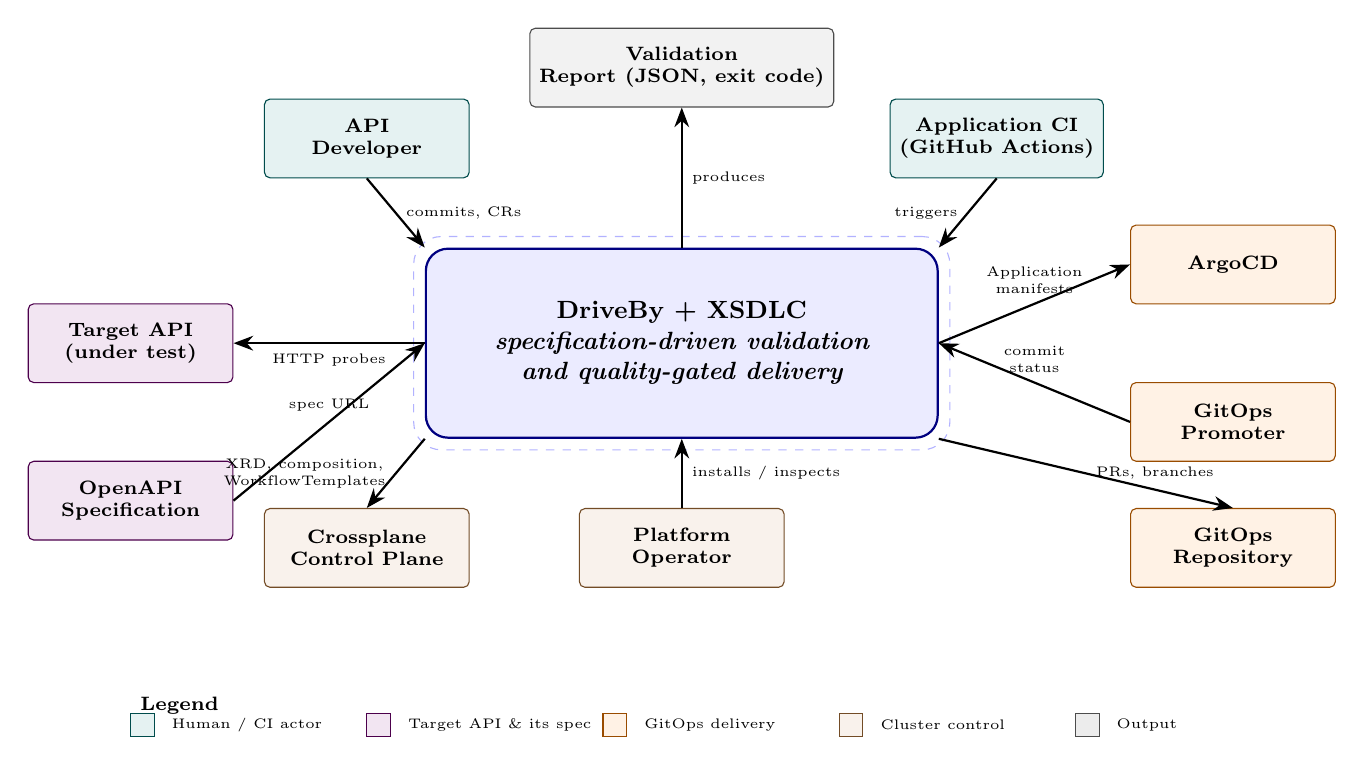
\begin{tikzpicture}[
    >={Stealth[length=2.5mm]},
    sysbox/.style={
        rectangle,
        rounded corners=8pt,
        draw=blue!50!black,
        thick,
        fill=blue!8,
        minimum width=6.5cm,
        minimum height=2.4cm,
        font=\bfseries\small,
        align=center
    },
    actor/.style={
        rectangle,
        rounded corners=2pt,
        draw=#1!60!black,
        fill=#1!10,
        minimum width=2.6cm,
        minimum height=1.0cm,
        font=\scriptsize\bfseries,
        align=center
    },
    flow/.style={
        ->,
        thick,
        font=\tiny,
        align=center
    }
]

% ---- The system under study (centre) ----
\node[sysbox] (sys) at (0,0) {DriveBy + XSDLC\\{\small\itshape specification-driven validation}\\{\small\itshape and quality-gated delivery}};

% ---- External actors / systems around the boundary ----
% North: developer, CI
\node[actor=teal]   (dev)     at (-4,2.6) {API\\Developer};
\node[actor=teal]   (ci)      at ( 4,2.6) {Application CI\\(GitHub Actions)};

% West: target API and its OpenAPI spec
\node[actor=violet] (api)     at (-7,0)   {Target API\\(under test)};
\node[actor=violet] (spec)    at (-7,-2)  {OpenAPI\\Specification};

% East: ArgoCD, Promoter, GitOps repo
\node[actor=orange] (argocd)  at ( 7,1)   {ArgoCD};
\node[actor=orange] (promoter)at ( 7,-1)  {GitOps\\Promoter};
\node[actor=orange] (gitops)  at ( 7,-2.6){GitOps\\Repository};

% South: Crossplane control plane and operator
\node[actor=brown]  (xplane)  at (-4,-2.6){Crossplane\\Control Plane};
\node[actor=brown]  (operator)at ( 0,-2.6){Platform\\Operator};

% North-east: the audience for the validation report
\node[actor=gray]   (report)  at ( 0,3.5) {Validation\\Report (JSON, exit code)};

% ---- Flows (label on every edge — what is exchanged) ----
\draw[flow] (dev.south)     -- node[right]{commits, CRs} (sys.north west);
\draw[flow] (ci.south)      -- node[left]{triggers}     (sys.north east);
\draw[flow] (sys.north)     -- node[right]{produces}    (report.south);

\draw[flow] (spec.east)     -- node[above]{spec URL}    (sys.west);
\draw[flow] (sys.west)      -- node[below]{HTTP probes}    (api.east);

\draw[flow] (sys.east)      -- node[above]{Application\\manifests} (argocd.west);
\draw[flow] (promoter.west) -- node[above]{commit\\status} (sys.east);
\draw[flow] (sys.south east)-- node[right]{PRs, branches}(gitops.north);

\draw[flow] (sys.south west)-- node[left] {XRD, composition,\\WorkflowTemplates} (xplane.north);
\draw[flow] (operator.north)-- node[right]{installs / inspects} (sys.south);

% ---- System-boundary band ----
\begin{scope}[on background layer]
    \node[draw=blue!30, dashed, rounded corners=10pt, fit=(sys), inner sep=4pt] (boundary) {};
\end{scope}

% ---- Legend (colour semantics) ----
\node[font=\scriptsize\bfseries, anchor=west] at (-7,-4.6) {Legend};
\begin{scope}[shift={(-7,-5.0)}]
  \fill[teal!10,draw=teal!60!black]   (0.0,0.0) rectangle (0.3,0.3);
  \node[font=\tiny, anchor=west] at (0.4,0.15) {Human / CI actor};
  \fill[violet!10,draw=violet!60!black] (3.0,0.0) rectangle (3.3,0.3);
  \node[font=\tiny, anchor=west] at (3.4,0.15) {Target API \& its spec};
  \fill[orange!10,draw=orange!60!black] (6.0,0.0) rectangle (6.3,0.3);
  \node[font=\tiny, anchor=west] at (6.4,0.15) {GitOps delivery};
  \fill[brown!10,draw=brown!60!black]  (9.0,0.0) rectangle (9.3,0.3);
  \node[font=\tiny, anchor=west] at (9.4,0.15) {Cluster control};
  \fill[gray!15,draw=gray!60!black]    (12.0,0.0) rectangle (12.3,0.3);
  \node[font=\tiny, anchor=west] at (12.4,0.15) {Output};
\end{scope}

\end{tikzpicture}
%
}
\caption{System context. The dashed boundary encloses the system under study (DriveBy CLI plus XSDLC composition). External actors and systems are coloured by category (legend at lower-left). Edge labels indicate the artifact or signal exchanged across the boundary.}
\label{fig:system-context}
\end{figure}

Figure~\ref{fig:component-diagram} then opens that boundary to expose the major internal Go packages of the CLI and their dependencies, and Figure~\ref{fig:class-diagram} (Section~\ref{sec:principle-checker-pattern}) shows the two central interfaces---\texttt{APISpec} and \texttt{PrincipleChecker}---together with their concrete realisations.

% ============================================================================
\section{Architecture Overview}
\label{sec:arch-overview}
% ============================================================================

% ----------------------------------------------------------------------------
\subsection{Design Goals}
\label{subsec:design-goals}
% ----------------------------------------------------------------------------

The DriveBy architecture is shaped by five design goals derived from the SDT axioms:

\begin{enumerate}
    \item \textbf{Version agnosticism.} Principle checkers must operate identically on OpenAPI~3.0.x, OpenAPI~3.1.0, and Swagger~2.0 specifications. No checker may contain version-specific branching logic.

    \item \textbf{Extensibility.} Adding a new validation principle must not require modifying existing checkers or the engine. The architecture must support open extension without closed modification.

    \item \textbf{Determinism by construction.} Static validation must be free of side effects, randomness, and environment-dependent behavior. The engine must produce identical reports given identical inputs.

    \item \textbf{Machine-readable output.} All validation output must be structured JSON suitable for consumption by CI/CD pipelines, quality dashboards, and downstream tooling.

    \item \textbf{Separation of concerns.} Type definitions, specification parsing, validation logic, runtime testing, report generation, and CLI presentation must reside in distinct packages with unidirectional dependencies.
\end{enumerate}

These goals map directly to the SDT axioms. Version agnosticism enables Completeness (the same checks apply regardless of specification version). Determinism by construction enforces the Axiom of Determinism. Machine-readable output satisfies Observability.

The implementation draws on two classical design patterns~\cite{gof}. The \textit{Adapter pattern} provides version agnosticism: each specification format is wrapped by an adapter that exposes a common interface. The \textit{Strategy pattern} provides extensibility: each principle checker is an interchangeable strategy that the engine selects based on validation mode.

% ----------------------------------------------------------------------------
\subsection{Module and Dependency Structure}
\label{subsec:module-structure}
% ----------------------------------------------------------------------------

DriveBy is implemented as a single Go module (\texttt{github.com/\allowbreak meter-peter/\allowbreak driveby/\allowbreak driveby-cli}). The module is organized into eleven internal packages with a strict, unidirectional dependency flow:

\begin{verbatim}
types <- spec <- loader <- principles <- testing <- engine <- cli
\end{verbatim}

No package may import a package to its left. The \texttt{types} package has zero internal dependencies, ensuring that data structures can be shared across all layers without introducing cycles. Figure~\ref{fig:dependency-flow} visualises this strict left-to-right dependency chain at the package level. Figure~\ref{fig:component-diagram} adds the external interfaces (the OpenAPI input, the target API under HTTP probing, and the structured report output) and groups packages into architectural layers.

\begin{figure}[htbp]
\centering
% Package Dependency Graph — Chapter 4
% Shows: types <- spec <- loader <- principles <- testing <- engine <- cli
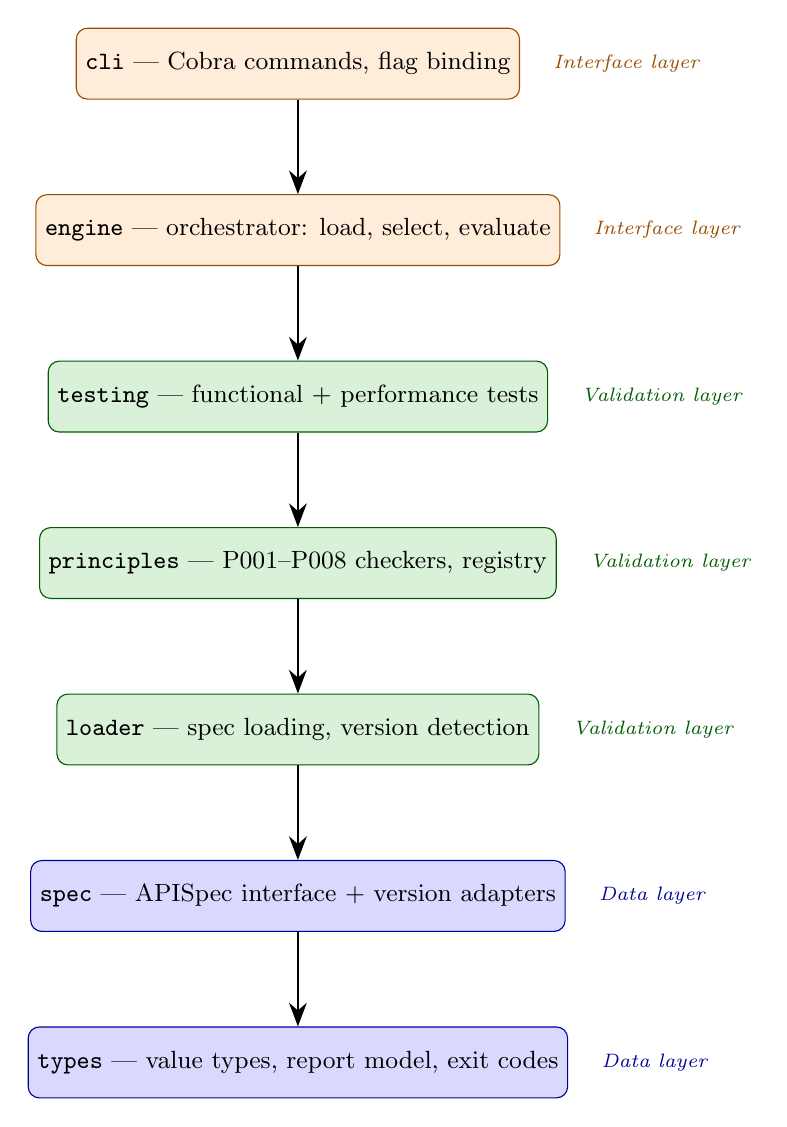
\begin{tikzpicture}[
    node distance=1.2cm,
    >={Stealth[length=3mm]},
    box/.style={
        rectangle,
        rounded corners=4pt,
        draw=#1!60!black,
        fill=#1!15,
        minimum width=5.5cm,
        minimum height=0.9cm,
        font=\small,
        align=center
    },
    layer label/.style={
        font=\scriptsize\itshape,
        text=#1!60!black,
        anchor=west
    }
]

% Nodes — bottom to top (import direction is upward)
\node[box=blue]   (types)      {\texttt{types} \textemdash\ value types, report model, exit codes};
\node[box=blue]   (spec)       [above=of types] {\texttt{spec} \textemdash\ APISpec interface + version adapters};
\node[box=green!60!black]  (loader)     [above=of spec] {\texttt{loader} \textemdash\ spec loading, version detection};
\node[box=green!60!black]  (principles) [above=of loader] {\texttt{principles} \textemdash\ P001--P008 checkers, registry};
\node[box=green!60!black]  (testing)    [above=of principles] {\texttt{testing} \textemdash\ functional + performance tests};
\node[box=orange] (engine)     [above=of testing] {\texttt{engine} \textemdash\ orchestrator: load, select, evaluate};
\node[box=orange] (cli)        [above=of engine] {\texttt{cli} \textemdash\ Cobra commands, flag binding};

% Arrows (import direction: upward)
\draw[->,thick] (spec)       -- (types);
\draw[->,thick] (loader)     -- (spec);
\draw[->,thick] (principles) -- (loader);
\draw[->,thick] (testing)    -- (principles);
\draw[->,thick] (engine)     -- (testing);
\draw[->,thick] (cli)        -- (engine);

% Layer labels on the right
\node[layer label=blue]          at ($(types.east)+(0.3,0)$)      {Data layer};
\node[layer label=blue]          at ($(spec.east)+(0.3,0)$)       {Data layer};
\node[layer label=green!60!black] at ($(loader.east)+(0.3,0)$)     {Validation layer};
\node[layer label=green!60!black] at ($(principles.east)+(0.3,0)$) {Validation layer};
\node[layer label=green!60!black] at ($(testing.east)+(0.3,0)$)    {Validation layer};
\node[layer label=orange]        at ($(engine.east)+(0.3,0)$)     {Interface layer};
\node[layer label=orange]        at ($(cli.east)+(0.3,0)$)        {Interface layer};

\end{tikzpicture}

\caption{DriveBy package dependency graph. Arrows indicate import direction; colour denotes architectural layer.}
\label{fig:dependency-flow}
\end{figure}

\begin{figure}[htbp]
\centering
\resizebox{\textwidth}{!}{% Component Diagram — Chapter 4 (DriveBy CLI internal components)
% Updated 2026-05 (round-1 review): compact natural-width layout (no resize),
% wider package nodes so labels fit without clipping.
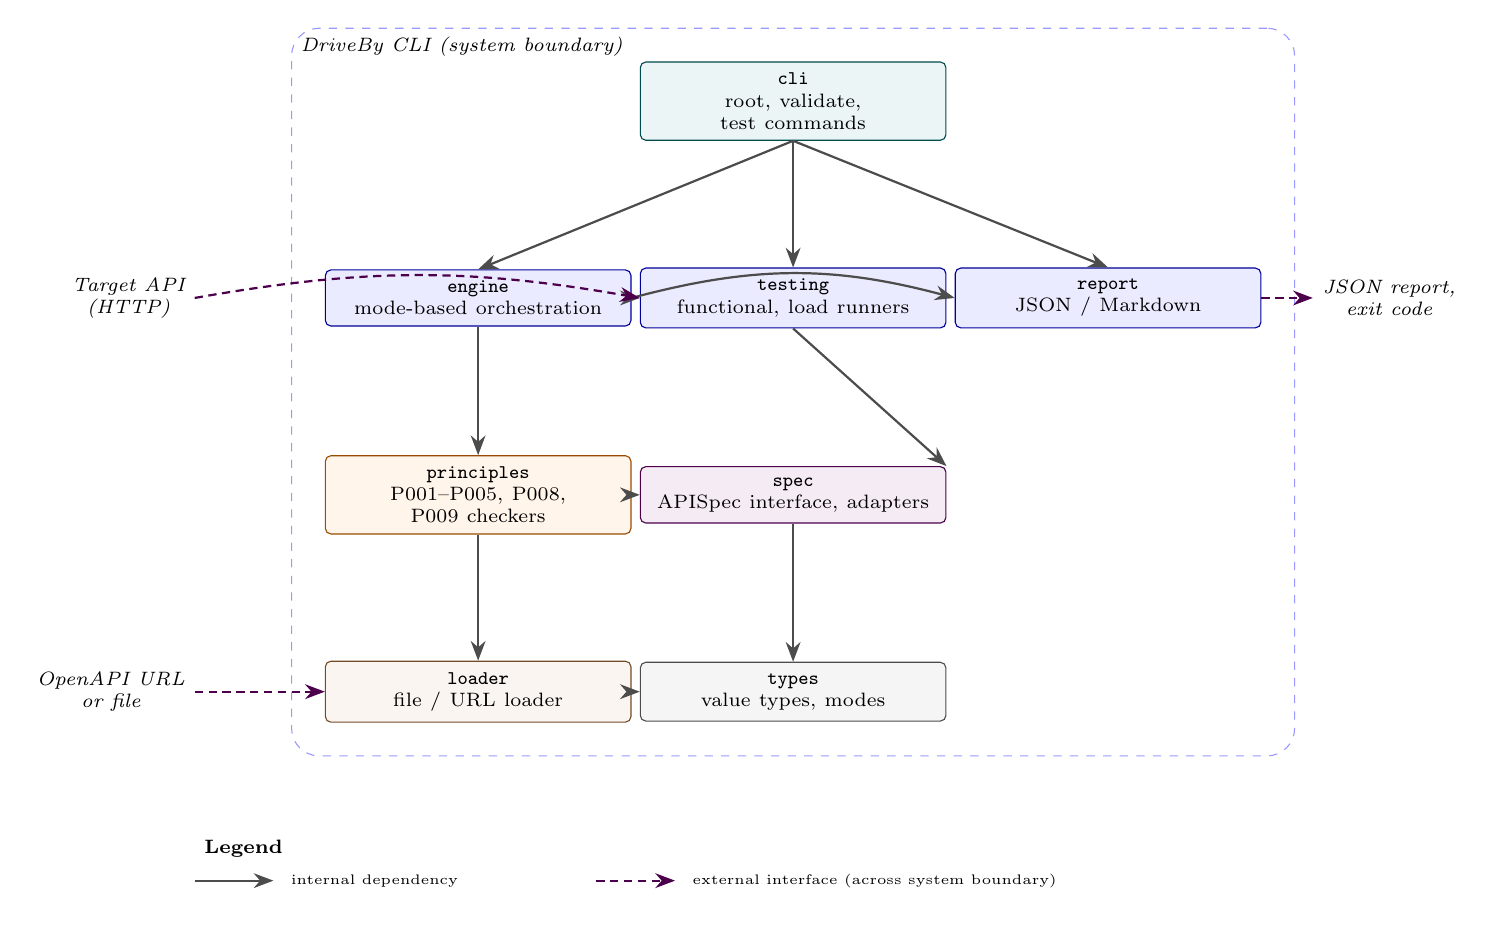
\begin{tikzpicture}[
    >={Stealth[length=2.5mm]},
    every node/.style={font=\scriptsize},
    pkg/.style={
        rectangle,
        rounded corners=2pt,
        draw=#1!60!black,
        fill=#1!8,
        align=center,
        text width=3.6cm,
        inner sep=4pt,
        font=\scriptsize\bfseries
    },
    dep/.style={->, thick, gray!60!black},
    ext/.style={->, thick, densely dashed, violet!60!black},
    extlabel/.style={font=\scriptsize\itshape, align=center}
]

% Top: CLI
\node[pkg=teal] (cli)        at (0,0)   {\texttt{cli}\\\mdseries\scriptsize\textnormal{root, validate, test commands}};

% Layer 2: orchestration
\node[pkg=blue] (engine)     at (-4.0,-2.5) {\texttt{engine}\\\mdseries\scriptsize\textnormal{mode-based orchestration}};
\node[pkg=blue] (testing)    at ( 0,-2.5)   {\texttt{testing}\\\mdseries\scriptsize\textnormal{functional, load runners}};
\node[pkg=blue] (report)     at ( 4.0,-2.5) {\texttt{report}\\\mdseries\scriptsize\textnormal{JSON / Markdown}};

% Layer 3: principles
\node[pkg=orange] (principles) at (-4.0,-5.0)
  {\texttt{principles}\\\mdseries\scriptsize\textnormal{P001--P005, P008, P009 checkers}};

% Layer 4: spec abstraction
\node[pkg=violet] (spec)     at (0,-5.0)   {\texttt{spec}\\\mdseries\scriptsize\textnormal{APISpec interface, adapters}};

% Layer 5: foundation
\node[pkg=brown]  (loader)   at (-4.0,-7.5)  {\texttt{loader}\\\mdseries\scriptsize\textnormal{file / URL loader}};
\node[pkg=gray]   (types)    at ( 0,-7.5)   {\texttt{types}\\\mdseries\scriptsize\textnormal{value types, modes}};

% Internal dependencies
\draw[dep] (cli.south)         -- (engine.north);
\draw[dep] (cli.south)         -- (testing.north);
\draw[dep] (cli.south)         -- (report.north);

\draw[dep] (engine.south)      -- (principles.north);
\draw[dep] (engine.east)       -- (testing.west);
\draw[dep] (engine.east)       to[bend left=15] (report.west);

\draw[dep] (principles.east)   -- (spec.west);
\draw[dep] (testing.south)     -- (spec.north east);

\draw[dep] (spec.south)        -- (types.north);
\draw[dep] (principles.south)  -- (loader.north);
\draw[dep] (loader.east)       -- (types.west);

% External interfaces (dashed, into/out of system boundary)
\node[extlabel, anchor=east] (ext-in)  at (-7.6,-7.5)   {OpenAPI URL\\or file};
\draw[ext] (ext-in.east) -- (loader.west);

\node[extlabel, anchor=east] (ext-api) at (-7.6,-2.5)   {Target API\\(HTTP)};
\draw[ext] (ext-api.east) to[bend left=10] (testing.west);

\node[extlabel, anchor=west] (ext-out) at ( 6.6,-2.5)   {JSON report,\\exit code};
\draw[ext] (report.east) -- (ext-out.west);

% System boundary (around all internal packages only)
\begin{scope}[on background layer]
    \node[draw=blue!40, dashed, rounded corners=10pt,
          fit=(cli)(engine)(testing)(report)(principles)(spec)(loader)(types),
          inner sep=12pt,
          label={[anchor=north west,font=\scriptsize\itshape]north west:DriveBy CLI (system boundary)}] {};
\end{scope}

% Legend
\node[anchor=west, font=\scriptsize\bfseries] at (-7.6,-9.5) {Legend};
\draw[dep]  (-7.6,-9.9) -- (-6.6,-9.9);
\node[anchor=west, font=\tiny] at (-6.5,-9.9) {internal dependency};
\draw[ext]  (-2.5,-9.9) -- (-1.5,-9.9);
\node[anchor=west, font=\tiny] at (-1.4,-9.9) {external interface (across system boundary)};

\end{tikzpicture}
}
\caption{Component diagram of the DriveBy CLI. Solid arrows are internal package dependencies; dashed violet arrows cross the system boundary to external interfaces. Colour denotes architectural layer (entry point, orchestration, principles, spec abstraction, foundation).}
\label{fig:component-diagram}
\end{figure}

Table~\ref{tab:package-map} summarizes each package's responsibility and size.

\begin{table}[htbp]
\centering
\caption{Package map of the DriveBy CLI.}
\label{tab:package-map}
\small
\begin{tabular}{@{}llr@{}}
\toprule
\textbf{Package} & \textbf{Responsibility} & \textbf{LOC} \\
\midrule
\texttt{types}      & Value types, report model, exit codes, config     & 655 \\
\texttt{spec}       & \texttt{APISpec} interface + version-specific adapters     & 831 \\
\texttt{loader}     & Specification loading, version detection, preprocessing & 322 \\
\texttt{principles} & Principle checkers (P001--P008), registry        & 1{,}690 \\
\texttt{testing}    & Runtime functional and performance testing        & 860 \\
\texttt{engine}     & Orchestrator: load, select, evaluate, aggregate   & 117 \\
\texttt{report}     & JSON and Markdown report generation               & 670 \\
\texttt{cli}        & Cobra command tree, flag binding, config assembly & 907 \\
\texttt{util}       & Preprocessing utilities (nullable, exclusive min/max) & 81 \\
\texttt{github}     & GitHub API client: PR comments, commit statuses   & 873 \\
\texttt{logger}     & Structured logging initialization                 & 164 \\
\bottomrule
\end{tabular}
\end{table}

The dependency flow enforces a clean separation of concerns. The \texttt{types} package defines \textit{what} validation produces. The \texttt{spec} package defines \textit{what} validation consumes. The \texttt{principles} package defines \textit{how} validation runs. The \texttt{engine} package \textit{orchestrates} the process. The \texttt{cli} package \textit{exposes} it to users.

% ============================================================================
\section{The Type System}
\label{sec:type-system}
% ============================================================================

The \texttt{types} package defines all value types shared across the framework. It has zero internal imports, making it the foundation layer that all other packages depend on.

% ----------------------------------------------------------------------------
\subsection{Value Types}
\label{subsec:value-types}
% ----------------------------------------------------------------------------

Two core enumerations govern the framework's behavior: \texttt{ValidationMode} controls which principles are evaluated, and the exit code constants control the CLI's return value.

\begin{lstlisting}[language=Go,caption={ValidationMode and exit code definitions (\texttt{types/modes.go}).},label={lst:modes}]
type ValidationMode string

const (
    ValidationModeStrict   ValidationMode = "strict"
    ValidationModeMinimal  ValidationMode = "minimal"
    ValidationModeTestOnly ValidationMode = "test-only"
    ValidationModeTestReady ValidationMode = "test-ready"
)

const (
    ExitSuccess          = 0  // All checks passed
    ExitValidationFailed = 1  // Validation or tests failed
    ExitExecutionError   = 2  // Runtime error
    ExitInvalidArgs      = 3  // Invalid CLI arguments
)
\end{lstlisting}

The four validation modes correspond directly to the modes defined in Section~\ref{sec:validation-modes} of Chapter~\ref{ch:methodology}. The exit code protocol enables CI/CD pipelines to distinguish between validation failures (exit~1, actionable) and execution errors (exit~2, infrastructure issues), a distinction that is critical for quality gate decisions.

The \texttt{types} package also defines \texttt{TestMode} (none, functional, performance, all) and \texttt{TestStatus} (passed, failed, warning, skipped, incomplete), which govern the runtime testing subsystem described in Section~\ref{sec:runtime-testing}.

% ----------------------------------------------------------------------------
\subsection{Validation Report Model}
\label{subsec:report-model}
% ----------------------------------------------------------------------------

The \texttt{ValidationReport} struct is the central output artifact of every DriveBy run. It aggregates per-principle results, summary statistics, and optional test results into a single JSON-serializable structure.

\begin{lstlisting}[language=Go,caption={ValidationReport and PrincipleResult (\texttt{types/report.go}).},label={lst:report}]
type ValidationReport struct {
    Status       string            `json:"status"`
    ExitCode     int               `json:"exit_code"`
    Version      string            `json:"version"`
    Environment  string            `json:"environment"`
    Timestamp    time.Time         `json:"timestamp"`
    Principles   []PrincipleResult `json:"principles"`
    TotalChecks  int               `json:"total_checks"`
    PassedChecks int               `json:"passed_checks"`
    FailedChecks int               `json:"failed_checks"`
    Summary      ValidationSummary `json:"summary"`
    TestResults  *TestResults      `json:"test_results,omitempty"`
}

type PrincipleResult struct {
    Principle    Principle
    Passed       bool
    Message      string
    Details      interface{}
    SuggestedFix string
    TestImpact   *TestImpact
}
\end{lstlisting}

The \texttt{PrincipleResult} struct captures not only the pass/fail status but also a human-readable message, structured details (type-dependent per principle), a suggested remediation, and the impact on downstream testing. The \texttt{TestImpact} field connects static validation to runtime testing: when a critical principle fails, the impact assessment indicates whether functional or performance tests can proceed and which endpoints are affected.

The \texttt{Principle} struct itself carries metadata---ID, name, description, category, severity, tags, and the list of checks---enabling the report to be self-documenting. A consumer of the JSON report can understand what was validated without consulting external documentation.

% ============================================================================
\section{The Specification Abstraction Layer}
\label{sec:spec-abstraction}
% ============================================================================

The specification abstraction layer is the architectural centerpiece of DriveBy. It decouples all validation logic from the concrete specification format, enabling version-agnostic principle checking.

% ----------------------------------------------------------------------------
\subsection{The APISpec Interface}
\label{subsec:apispec-interface}
% ----------------------------------------------------------------------------

The \texttt{APISpec} interface defines a version-agnostic view over any API specification. All principle checkers and the engine receive an \texttt{APISpec} value; they never interact with the raw kin-openapi~\cite{kin-openapi} types (\texttt{*openapi3.T}, \texttt{*openapi2.T}).

\begin{lstlisting}[language=Go,caption={The APISpec interface (\texttt{spec/spec.go}).},label={lst:apispec}]
type APISpec interface {
    Type() SpecType
    RawVersion() string
    Info() *SpecInfo
    Paths() map[string]*PathItem
    Components() *Components
    Security() []SecurityRequirement
    ValidateStructure(ctx context.Context) error
}
\end{lstlisting}

The interface is intentionally minimal. It exposes only the concepts that DriveBy's validators need: metadata (\texttt{Info}), the operation tree (\texttt{Paths}), reusable definitions (\texttt{Components}), global security requirements (\texttt{Security}), and a structural validation hook (\texttt{ValidateStructure}). The \texttt{Type} and \texttt{RawVersion} methods allow callers to inspect the specification flavour when necessary (e.g., P001's null type check), but principle checkers are strongly discouraged from branching on version.

This design realizes the Adapter pattern~\cite{gof}: each specification format provides its own adapter that translates native types into the normalized \texttt{APISpec} interface. Adding support for a new specification format (e.g., AsyncAPI) requires implementing the interface without modifying any existing checker.

% ----------------------------------------------------------------------------
\subsection{Normalized Types}
\label{subsec:normalized-types}
% ----------------------------------------------------------------------------

The \texttt{APISpec} interface returns normalized types that abstract away version-specific representation differences. Table~\ref{tab:normalized-types} lists the key types and their purpose.

\begin{table}[htbp]
\centering
\caption{Normalized specification types in the \texttt{spec} package.}
\label{tab:normalized-types}
\footnotesize
\begin{tabular}{@{}p{2.4cm}p{4.6cm}p{5.8cm}@{}}
\toprule
\textbf{Type} & \textbf{Key Fields} & \textbf{Purpose} \\
\midrule
\texttt{Schema}       & Type, Properties, Required, AllOf/OneOf/AnyOf, Nullable & Unified schema representation; handles both 3.0.x \texttt{nullable} and 3.1.0 \texttt{type: [``null'', ...]} semantics. \\
\texttt{Operation}    & Method, Path, Parameters, RequestBody, Responses, Security & Single HTTP operation with all metadata needed by checkers. \\
\texttt{PathItem}     & Parameters, Operations map & Groups operations sharing a path; path-level parameters are propagated. \\
\texttt{Parameter}    & Name, In, Required, Schema, Example & Normalized parameter; \texttt{In} is a string (``path'', ``query'', ``header'', ``cookie''). \\
\texttt{Response}     & Description, Content map & Status-code-keyed response with content-type-specific schemas. \\
\texttt{SecurityScheme} & Type, Name, In, Scheme, Description & Auth mechanism metadata for P005 validation. \\
\texttt{Components}   & Schemas, Responses, SecuritySchemes & Reusable definitions referenced across operations. \\
\bottomrule
\end{tabular}
\end{table}

The \texttt{Schema} type deserves particular attention. It normalizes the three composition mechanisms (allOf, oneOf, anyOf) into slice fields, handles nullable semantics across OpenAPI versions, and recursively normalizes nested properties and array items. This recursive normalization ensures that principle checkers like P004 (Schema Definitions) can traverse the full schema tree without version-specific logic.

% ----------------------------------------------------------------------------
\subsection{Version-Specific Adapters}
\label{subsec:version-adapters}
% ----------------------------------------------------------------------------

Two adapters implement the \texttt{APISpec} interface: \texttt{openAPI3Spec} for OpenAPI~3.0.x and 3.1.0, and \texttt{swagger2Spec} for Swagger~2.0. Both are constructed by the loader (Section~\ref{sec:loading}) and wrap the kin-openapi library's~\cite{kin-openapi} native document types.

The OpenAPI~3.x adapter (\texttt{openapi3.go}, 324~LOC) performs the bulk of the normalization work. Listing~\ref{lst:normalize-schema} shows an excerpt from the schema normalization function, which recursively translates a kin-openapi \texttt{*openapi3.Schema} into the normalized \texttt{spec.Schema}.

\begin{lstlisting}[language=Go,caption={Schema normalization excerpt (\texttt{spec/openapi3.go}).},label={lst:normalize-schema}]
func normalizeSchema(s *openapi3.Schema) *Schema {
    if s == nil { return nil }
    out := &Schema{
        Type: s.Type, Format: s.Format,
        MinLength: s.MinLength, MaxLength: s.MaxLength,
        Pattern: s.Pattern, Min: s.Min, Max: s.Max,
        Enum: s.Enum, Required: append([]string{}, s.Required...),
        Description: s.Description, Nullable: s.Nullable,
    }
    for name, prop := range s.Properties {
        if prop != nil && prop.Value != nil {
            out.Properties[name] = normalizeSchema(prop.Value)
        }
    }
    for _, ref := range s.AllOf {
        if ref != nil && ref.Value != nil {
            out.AllOf = append(out.AllOf, normalizeSchema(ref.Value))
        }
    }
    return out
}
\end{lstlisting}

The Swagger~2.0 adapter (\texttt{swagger2.go}, 293~LOC) performs analogous normalization but must account for Swagger-specific conventions: parameters with \texttt{in: body} are translated to \texttt{RequestBody}, security definitions map to \texttt{SecurityScheme}, and the single-host model is normalized to match the OpenAPI~3.x multi-server paradigm. The structural validation for Swagger~2.0 is implemented as a focused set of sanity checks rather than full schema validation, since kin-openapi does not provide a \texttt{Validate()} method for Swagger~2.0 documents.

% ----------------------------------------------------------------------------
\subsection{Schema Composition Handling}
\label{subsec:schema-composition}
% ----------------------------------------------------------------------------

OpenAPI specifications frequently use \texttt{allOf} to compose schemas---combining a base model with additional properties. Principle checkers that need a flat view of all properties (e.g., P004's required-field validation) would need to recursively merge \texttt{allOf} members, duplicating logic across checkers.

The \texttt{FlattenAllOf} utility in \texttt{spec.go} centralizes this concern. It takes a \texttt{*Schema} with \texttt{allOf} members and returns a merged schema where all properties and required fields from all members are combined into a single level. If the parent schema has no \texttt{allOf}, it is returned unchanged. This utility is used by both the P004 checker and the functional testing subsystem (Section~\ref{sec:runtime-testing}) when generating example request bodies from composed schemas.

% ============================================================================
\section{Specification Loading and Preprocessing}
\label{sec:loading}
% ============================================================================

The \texttt{loader} package is responsible for loading API specifications from files or URLs, detecting the specification format, applying compatibility preprocessing, and constructing the appropriate \texttt{APISpec} adapter.

% ----------------------------------------------------------------------------
\subsection{Source Detection and Version Dispatch}
\label{subsec:version-dispatch}
% ----------------------------------------------------------------------------

The loader accepts specifications from local files or HTTP URLs. The \texttt{LoadFromFileOrURL} method detects the source type by inspecting the path prefix (\texttt{http://} or \texttt{https://}) and delegates to file reading or HTTP fetching accordingly.

After obtaining the raw bytes, the loader performs version detection by unmarshalling into a generic \texttt{map[string]interface\{\}} and inspecting two discriminator fields:

\begin{lstlisting}[language=Go,caption={Specification version detection (\texttt{loader/loader.go}).},label={lst:version-detect}]
func (l *Loader) loadFromData(source string, data []byte) error {
    var raw map[string]interface{}
    if err := json.Unmarshal(data, &raw); err != nil {
        return fmt.Errorf("failed to parse spec: %w", err)
    }
    // OpenAPI 3.x: has "openapi" field
    if ver, ok := raw["openapi"].(string); ok && ver != "" {
        util.PreprocessNullableAnyOf(raw)
        util.PreprocessExclusiveMinMax(raw)
        processed, _ := json.Marshal(raw)
        doc, err := openapi3.NewLoader().LoadFromData(processed)
        if err != nil { return err }
        l.doc = spec.NewOpenAPI3Spec(doc)
        return nil
    }
    // Swagger 2.0: has "swagger" field with value "2.0"
    if ver, ok := raw["swagger"].(string); ok && ver == "2.0" {
        var doc openapi2.T
        json.Unmarshal(data, &doc)
        l.doc = spec.NewSwagger2Spec(&doc)
        return nil
    }
    return fmt.Errorf("unsupported spec format: %s", source)
}
\end{lstlisting}

This approach---unmarshal once into a generic map, inspect a discriminator field, then unmarshal again into the typed struct---avoids speculative parsing with multiple libraries. The preprocessing step (lines 7--9 in Listing~\ref{lst:version-detect}) is applied only to OpenAPI~3.x specifications and is described in the next section.

% ----------------------------------------------------------------------------
\subsection{Compatibility Preprocessing}
\label{subsec:preprocessing}
% ----------------------------------------------------------------------------

The kin-openapi library~\cite{kin-openapi} provides comprehensive support for OpenAPI~3.0.x but has limitations with certain OpenAPI~3.1.0 constructs. DriveBy addresses this through two preprocessing transforms applied to the raw JSON before kin-openapi parses it.

\textbf{PreprocessNullableAnyOf.} OpenAPI~3.1.0 represents nullable types as \texttt{anyOf: [\{type: X\}, \{type: null\}]}. The kin-openapi library rejects \texttt{type: null}, causing valid 3.1.0 specifications to fail loading. The preprocessor detects two-member \texttt{anyOf} arrays where one member is \texttt{\{type: null\}} and rewrites them to the OpenAPI~3.0.x equivalent: the concrete type with \texttt{nullable: true}. This transformation is applied recursively to all schema definitions in the document.

\textbf{PreprocessExclusiveMinMax.} OpenAPI~3.1.0 adopted JSON Schema 2020-12 semantics where \texttt{exclusiveMinimum} and \texttt{exclusiveMaximum} are numeric values. OpenAPI~3.0.x uses boolean values paired with \texttt{minimum}/\texttt{maximum}. The preprocessor converts numeric exclusive bounds to booleans when paired with their non-exclusive counterparts, and removes them otherwise.

Both transforms operate on the raw \texttt{map[string]interface\{\}} before any typed parsing occurs. This ensures that the kin-openapi library receives a document it can parse, while preserving the semantic content of the original specification. The approach trades strict 3.1.0 fidelity for broad compatibility---a pragmatic choice given that kin-openapi is the most mature OpenAPI parser available for Go.

% ============================================================================
\section{The Principle Checker Pattern}
\label{sec:principle-checker}
\label{sec:principle-checker-pattern}
% ============================================================================

The two design abstractions introduced so far---the \texttt{APISpec} interface (Section~\ref{sec:spec-abstraction}) and the \texttt{PrincipleChecker} interface defined below---are summarised together in Figure~\ref{fig:class-diagram}. The figure shows: the two interfaces with their methods; the two version-specific adapters that realise \texttt{APISpec} (\texttt{openAPI3Spec} and \texttt{swagger2Spec}); the seven implemented and two planned concrete principle checkers that realise \texttt{PrincipleChecker}; and how the \texttt{Engine} consumes both interfaces to drive validation.

\begin{figure}[htbp]
\centering
\resizebox{\textwidth}{!}{% Class / Interface Diagram — Chapter 4
% Updated 2026-05 (round-1 review): plain-rectangle layout (no rectangle split)
% to avoid renderer issues; compact natural-width coordinates.
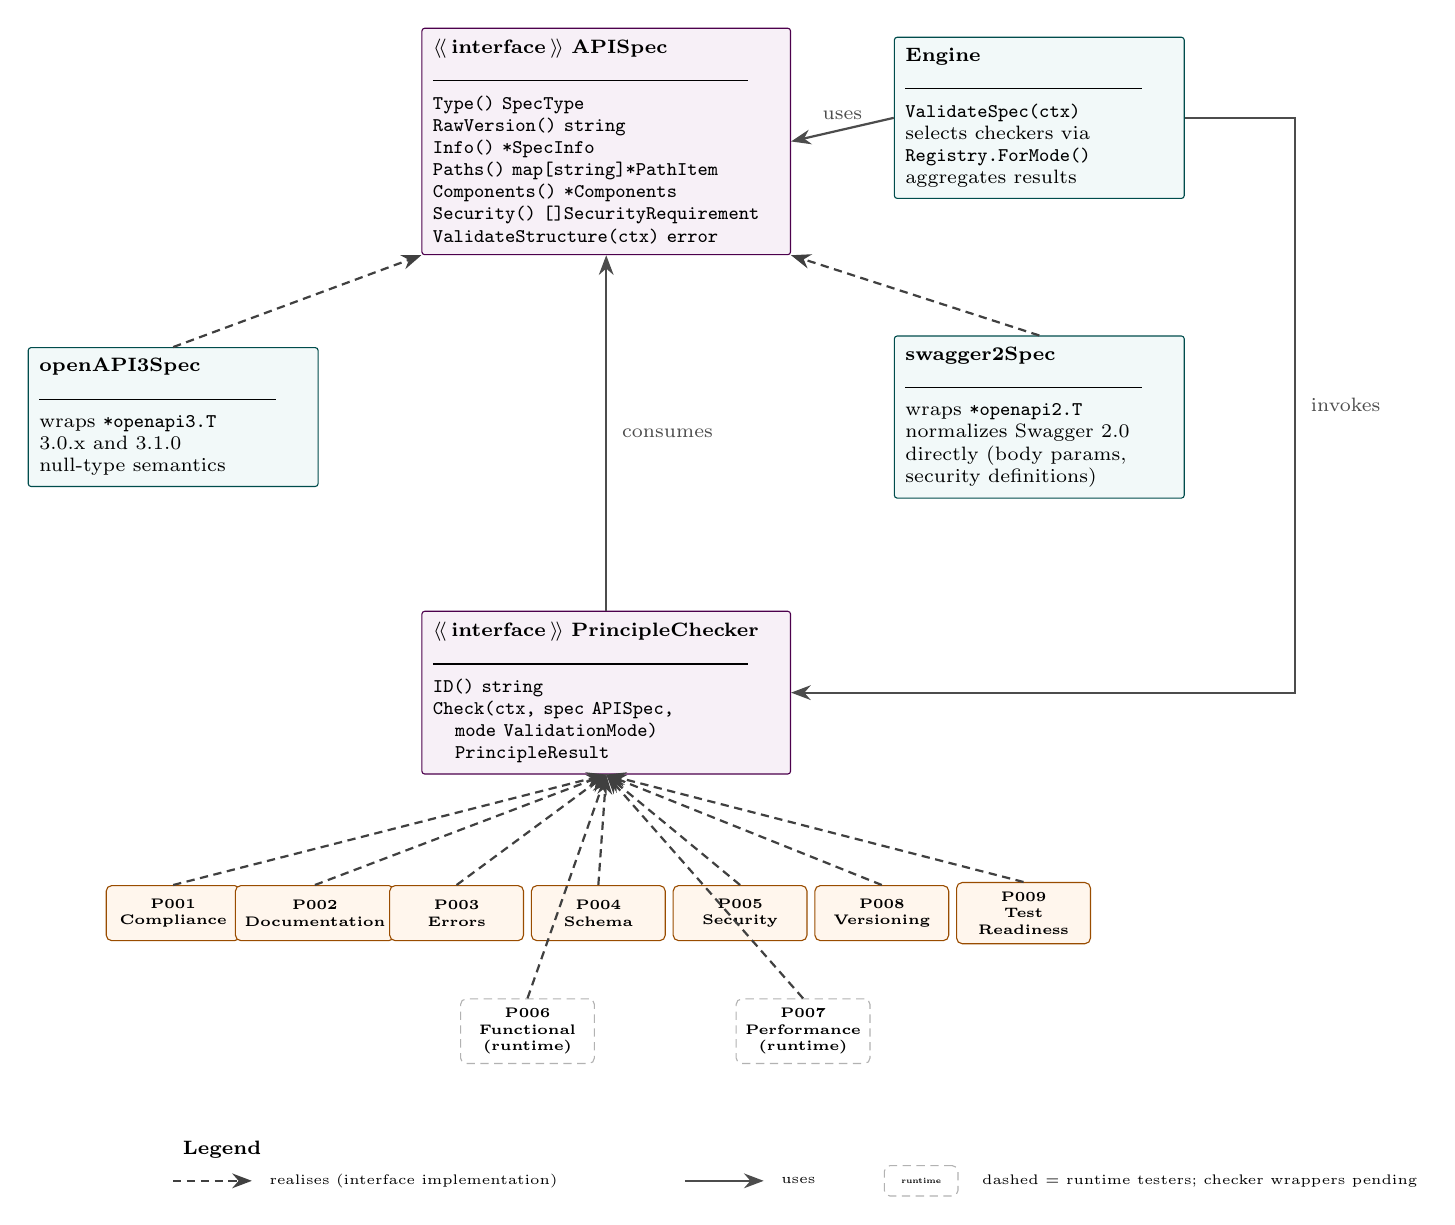
\begin{tikzpicture}[
    >={Stealth[length=2.5mm]},
    every node/.style={font=\scriptsize},
    iface/.style={
        rectangle,
        rounded corners=1pt,
        draw=violet!60!black,
        fill=violet!6,
        align=left,
        text width=4.4cm,
        inner sep=4pt,
        font=\scriptsize
    },
    cls/.style={
        rectangle,
        rounded corners=1pt,
        draw=teal!60!black,
        fill=teal!5,
        align=left,
        text width=3.4cm,
        inner sep=4pt,
        font=\scriptsize
    },
    plcheck/.style={
        rectangle,
        rounded corners=2pt,
        draw=orange!60!black,
        fill=orange!7,
        align=center,
        minimum width=1.7cm,
        minimum height=0.7cm,
        font=\tiny\bfseries
    },
    plcheck-planned/.style={
        rectangle,
        rounded corners=2pt,
        draw=gray!60,
        fill=white,
        align=center,
        minimum width=1.7cm,
        minimum height=0.7cm,
        densely dashed,
        font=\tiny\bfseries
    },
    realize/.style={->, thick, densely dashed, gray!50!black},
    use/.style={->, thick, gray!60!black}
]

% ==================== Top: APISpec interface and adapters + Engine ====================
\node[iface] (apispec) at (0,0) {%
  \textbf{$\langle\!\langle$\,interface\,$\rangle\!\rangle$ APISpec}\\[2pt]
  \rule{4cm}{0.4pt}\\[2pt]
  \texttt{Type() SpecType}\\
  \texttt{RawVersion() string}\\
  \texttt{Info() *SpecInfo}\\
  \texttt{Paths() map[string]*PathItem}\\
  \texttt{Components() *Components}\\
  \texttt{Security() []SecurityRequirement}\\
  \texttt{ValidateStructure(ctx) error}%
};

\node[cls] (oa3) at (-5.5,-3.5) {%
  \textbf{openAPI3Spec}\\[2pt]
  \rule{3cm}{0.4pt}\\[2pt]
  wraps \texttt{*openapi3.T}\\
  3.0.x and 3.1.0\\
  null-type semantics%
};

\node[cls] (sw2) at (5.5,-3.5) {%
  \textbf{swagger2Spec}\\[2pt]
  \rule{3cm}{0.4pt}\\[2pt]
  wraps \texttt{*openapi2.T}\\
  normalizes Swagger 2.0\\
  directly (body params,\\
  security definitions)%
};

\draw[realize] (oa3.north) -- (apispec.south west);
\draw[realize] (sw2.north) -- (apispec.south east);

% Engine to the right of APISpec, but stacked above to keep width contained
\node[cls] (engine) at (5.5,0.3) {%
  \textbf{Engine}\\[2pt]
  \rule{3cm}{0.4pt}\\[2pt]
  \texttt{ValidateSpec(ctx)}\\
  selects checkers via\\
  \texttt{Registry.ForMode()}\\
  aggregates results%
};
\draw[use] (engine.west) -- node[above]{uses} (apispec.east);

% ==================== Bottom: PrincipleChecker interface and impls ====================
\node[iface] (pcint) at (0,-7.0) {%
  \textbf{$\langle\!\langle$\,interface\,$\rangle\!\rangle$ PrincipleChecker}\\[2pt]
  \rule{4cm}{0.4pt}\\[2pt]
  \texttt{ID() string}\\
  \texttt{Check(ctx, spec APISpec,}\\
  \quad\texttt{mode ValidationMode)}\\
  \quad\texttt{PrincipleResult}%
};

\draw[use] (pcint.north) -- node[right,xshift=2pt]{consumes} (apispec.south);
% Route invokes-arrow around swagger2Spec via the right margin to avoid overlap.
\draw[use] (engine.east) -- ++(1.4,0) |- node[pos=0.25,right,xshift=2pt]{invokes} (pcint.east);

% Concrete principle checkers
\node[plcheck]         (p001) at (-5.5,-9.8) {P001\\Compliance};
\node[plcheck]         (p002) at (-3.7,-9.8) {P002\\Documentation};
\node[plcheck]         (p003) at (-1.9,-9.8) {P003\\Errors};
\node[plcheck]         (p004) at (-0.1,-9.8) {P004\\Schema};
\node[plcheck]         (p005) at ( 1.7,-9.8) {P005\\Security};
\node[plcheck]         (p008) at ( 3.5,-9.8) {P008\\Versioning};
\node[plcheck]         (p009) at ( 5.3,-9.8) {P009\\Test\\Readiness};
\node[plcheck-planned] (p006) at (-1.0,-11.3){P006\\Functional\\(runtime)};
\node[plcheck-planned] (p007) at ( 2.5,-11.3){P007\\Performance\\(runtime)};

\foreach \n in {p001,p002,p003,p004,p005,p008,p009,p006,p007} {
  \draw[realize] (\n.north) -- (pcint.south);
}

% Legend
\node[anchor=west, font=\scriptsize\bfseries] at (-5.5,-12.8) {Legend};
\draw[realize] (-5.5,-13.2) -- (-4.5,-13.2);
\node[anchor=west, font=\tiny] at (-4.4,-13.2) {realises (interface implementation)};
\draw[use] (1.0,-13.2) -- (2.0,-13.2);
\node[anchor=west, font=\tiny] at (2.1,-13.2) {uses};
\node[plcheck-planned, scale=0.55] at (4.0,-13.2) {runtime};
\node[anchor=west, font=\tiny] at (4.65,-13.2) {dashed = runtime testers; checker wrappers pending};

\end{tikzpicture}
}
\caption{Class / interface diagram of DriveBy's two central abstractions. Dashed grey arrows denote interface realisation (concrete class implements interface); solid grey arrows denote use. Dashed nodes (P006, P007) are defined theoretically but not yet implemented as \texttt{PrincipleChecker} wrappers.}
\label{fig:class-diagram}
\end{figure}

% ----------------------------------------------------------------------------
\subsection{The PrincipleChecker Interface}
\label{subsec:checker-interface}
% ----------------------------------------------------------------------------

Every SDT principle is implemented as a type that satisfies the \texttt{PrincipleChecker} interface:

\begin{lstlisting}[language=Go,caption={The PrincipleChecker interface (\texttt{principles/checker.go}).},label={lst:checker}]
type PrincipleChecker interface {
    ID() string
    Check(ctx context.Context, apiSpec spec.APISpec,
          mode types.ValidationMode) types.PrincipleResult
}
\end{lstlisting}

The interface is deliberately minimal. \texttt{ID()} returns the principle identifier (e.g., \texttt{"P001"}). \texttt{Check()} receives the normalized specification, the validation mode, and a context for cancellation, and returns a structured result. The \texttt{spec.APISpec} parameter enforces the abstraction boundary: checkers cannot access raw kin-openapi types.

This design realizes the Strategy pattern~\cite{gof}. Each checker is an interchangeable strategy that the engine selects based on validation mode. Adding a new principle requires implementing the interface and registering the checker; no existing code is modified.

% ----------------------------------------------------------------------------
\subsection{Checker Implementation Pattern}
\label{subsec:checker-implementation}
% ----------------------------------------------------------------------------

All seven implemented checkers follow a consistent internal pattern. Listing~\ref{lst:p001} shows an abbreviated version of P001 (OpenAPI Specification Compliance) to illustrate the pattern.

\begin{lstlisting}[language=Go,caption={P001 checker pattern (abbreviated, \texttt{principles/p001\_compliance.go}).},label={lst:p001}]
type P001Compliance struct{}

func (p *P001Compliance) ID() string { return "P001" }

func (p *P001Compliance) Check(ctx context.Context,
    doc spec.APISpec, mode types.ValidationMode,
) types.PrincipleResult {
    result := types.PrincipleResult{
        Principle: types.CorePrinciples[0],
        Passed: true, Details: make(map[string]interface{}),
    }
    checks := make(map[string]bool)
    // 1. Version check
    if doc.RawVersion() == "" {
        checks["Specification version is present"] = false
    }
    // 2. Info fields, 3. Paths, 4. Components ...
    // 5. Structural validation via adapter
    if err := doc.ValidateStructure(ctx); err != nil {
        checks["Specification structure is valid"] = false
    }
    // 6. Duplicate operationIds, 7. HTTP methods, 8. Null type
    // ... aggregate checks into result ...
    return result
}
\end{lstlisting}

The pattern has four steps: (1)~initialize a \texttt{PrincipleResult} with the principle metadata from \texttt{CorePrinciples}; (2)~execute individual checks against the \texttt{APISpec}, recording each as a named boolean; (3)~aggregate failures into the result's message and details; (4)~return the result. This consistency simplifies testing (each checker has a corresponding test file in \texttt{test/}) and makes the codebase predictable for contributors.

Table~\ref{tab:checker-implementations} lists all principle checker implementations with their check counts and sizes.

\begin{table}[htbp]
\centering
\caption{Principle checker implementations.}
\label{tab:checker-implementations}
\small
\begin{tabular}{@{}lllr@{}}
\toprule
\textbf{File} & \textbf{Principle} & \textbf{Checks} & \textbf{LOC} \\
\midrule
\texttt{p001\_compliance.go}   & P001: OpenAPI Compliance     & 7  & 180 \\
\texttt{p002\_documentation.go} & P002: Documentation Quality  & 10 & 197 \\
\texttt{p003\_errors.go}       & P003: Error Handling          & 7  & 234 \\
\texttt{p004\_schema.go}       & P004: Schema Definitions      & 10 & 432 \\
\texttt{p005\_security.go}     & P005: Security Standards      & 7  & 221 \\
\texttt{p008\_versioning.go}   & P008: Versioning Strategy     & 7  & 163 \\
\texttt{p009\_test\_readiness.go} & P009: Test Readiness          & 4  & 188 \\
\bottomrule
\end{tabular}
\end{table}

The check counts correspond to those enumerated in Section~\ref{sec:nine-principles} of Chapter~\ref{ch:methodology}. P004 is the largest checker because recursive schema traversal requires handling nested objects, arrays, allOf compositions, and enum validation at every level. P009 (Test Readiness) completes the seven-checker set, validating whether the specification provides sufficient examples and typed schemas for meaningful runtime testing.

% ----------------------------------------------------------------------------
\subsection{The Registry and Mode-Based Selection}
\label{subsec:registry}
% ----------------------------------------------------------------------------

The \texttt{Registry} manages all registered checkers and selects subsets based on validation mode. This centralizes the mode-to-checker mapping defined in Table~\ref{tab:validation-modes} (Chapter~\ref{ch:methodology}).

\begin{lstlisting}[language=Go,caption={Mode-based checker selection (\texttt{principles/registry.go}).},label={lst:formode}]
func NewRegistry() *Registry {
    return &Registry{
        checkers: []PrincipleChecker{
            &P001Compliance{}, &P002Documentation{},
            &P003Errors{}, &P004Schema{},
            &P005Security{}, &P008Versioning{},
            &P009TestReadiness{},
        },
    }
}

func (r *Registry) ForMode(mode types.ValidationMode) []PrincipleChecker {
    switch mode {
    case types.ValidationModeTestOnly:
        return nil
    case types.ValidationModeMinimal:
        return []PrincipleChecker{r.Get("P001")}
    case types.ValidationModeTestReady:
        return []PrincipleChecker{r.Get("P001"), r.Get("P002"), r.Get("P003"), r.Get("P004"), r.Get("P009")}
    case types.ValidationModeStrict:
        return []PrincipleChecker{
            r.Get("P001"), r.Get("P002"), r.Get("P003"),
            r.Get("P004"), r.Get("P005"), r.Get("P008"),
        }
    default:
        return []PrincipleChecker{r.Get("P001")}
    }
}
\end{lstlisting}

The \texttt{ForMode} method encodes the mode semantics from Section~\ref{sec:validation-modes}: minimal mode evaluates only P001; test-ready mode evaluates P001, P002 (test-critical documentation, excluding contact/license), P003 (error schemas for 4xx responses), P004 (type checks only), and P009; strict mode evaluates all six static principles (P001--P005, P008); test-only mode returns no static checkers, deferring entirely to the runtime testing subsystem. When P006 and P007 are implemented as \texttt{PrincipleChecker} wrappers, they will be added to the registry and included in the test-only and combined mode selections.

% ============================================================================
\section{The Validation Engine}
\label{sec:engine}
% ============================================================================

% ----------------------------------------------------------------------------
\subsection{Engine Configuration and Initialization}
\label{subsec:engine-config}
% ----------------------------------------------------------------------------

The \texttt{Engine} struct ties together the loader, the registry, and the user's configuration. It is the single entry point for all validation operations.

\begin{verbatim}
type Engine struct {
    config   types.ValidatorConfig
    loader   *loader.Loader
    registry *principles.Registry
}
\end{verbatim}

The \texttt{New} constructor validates the configuration (requiring a spec path, base URL, and positive timeout), sets a default validation mode of \texttt{minimal} if none is specified, and instantiates the loader and registry. This validation-at-construction approach ensures that the engine is always in a valid state when \texttt{ValidateSpec} is called.

% ----------------------------------------------------------------------------
\subsection{The Validation Pipeline}
\label{subsec:validation-pipeline}
% ----------------------------------------------------------------------------

The core validation pipeline is implemented in a single method, \texttt{ValidateSpec}, which executes four steps sequentially:

\begin{lstlisting}[language=Go,caption={The validation pipeline (\texttt{engine/engine.go}).},label={lst:validate-spec}]
func (e *Engine) ValidateSpec(ctx context.Context,
) (*types.ValidationReport, error) {
    // Step 1: Load and normalize the specification
    if err := e.loader.LoadFromFileOrURL(e.config.SpecPath); err != nil {
        return nil, fmt.Errorf("failed to load API spec: %w", err)
    }
    doc := e.loader.GetDocument()

    // Step 2: Initialize the report
    report := &types.ValidationReport{
        Version: e.config.Version, Environment: e.config.Environment,
        Timestamp: time.Now(),
    }

    // Step 3: Select and run principle checkers
    checkers := e.registry.ForMode(e.config.ValidationMode)
    for _, checker := range checkers {
        result := checker.Check(ctx, doc, e.config.ValidationMode)
        report.Principles = append(report.Principles, result)
        if result.Passed { report.PassedChecks++ } else {
            report.FailedChecks++ }
    }
    report.TotalChecks = len(checkers)

    // Step 4: Compute summary (critical issues, warnings, categories)
    updateSummary(report)
    return report, nil
}
\end{lstlisting}

Step~1 invokes the loader, which performs version detection, preprocessing, and adapter construction (Section~\ref{sec:loading}). Step~2 initializes the report with metadata from the engine's configuration. Step~3 iterates over the mode-selected checkers, invoking each with the normalized specification and accumulating results. Step~4 computes summary statistics---counts of critical issues, warnings, affected categories, and failed tags---that the report generator and CLI use for presentation.

The pipeline is deterministic by construction: given the same specification and mode, the same checkers run in the same order and produce the same results. The only non-deterministic element is the timestamp, which is metadata rather than validation output.

The engine also provides a \texttt{Validate} method that wraps \texttt{ValidateSpec} with logging output for backward compatibility. The CLI commands use \texttt{Validate} to write structured logs to stderr while the JSON report is written to stdout.

% ============================================================================
\section{Runtime Testing Subsystem}
\label{sec:runtime-testing}
% ============================================================================

While the principle checkers (P001--P005, P008) operate on the specification as a static document, the runtime testing subsystem validates the live API against its specification. The subsystem implements the logic that will underpin P006 (Functional Testing) and P007 (Performance Testing) once their \texttt{PrincipleChecker} wrappers are complete.

% ----------------------------------------------------------------------------
\subsection{Functional Testing}
\label{subsec:functional-testing}
% ----------------------------------------------------------------------------

The \texttt{FunctionalTester} in \texttt{testing/functional.go} (552~LOC) derives test cases from the specification and executes them against a live API instance. For each non-deprecated operation, the tester:

\begin{enumerate}
    \item \textbf{Substitutes path parameters} using examples from the specification or type-based defaults (e.g., UUID format generates a valid UUID, integer generates \texttt{1}).
    \item \textbf{Constructs request bodies} for POST, PUT, and PATCH operations by extracting examples from the specification or generating them from the schema definition, including recursive \texttt{allOf} flattening.
    \item \textbf{Adds authentication headers} when the user provides credentials (Bearer token, API key, or basic authentication).
    \item \textbf{Executes the request} with retry logic for transient failures (502, 503, 504) using exponential backoff.
    \item \textbf{Validates the response} by checking that the status code is documented in the specification and that the response body conforms to the declared schema (required fields, type checks).
\end{enumerate}

Authentication awareness is a distinctive feature. If the API returns a 401 status code and no authentication was configured, the endpoint is marked as \textit{skipped} rather than failed. This prevents false negatives when testing APIs that require authentication without credentials, while still reporting the authentication requirement.

The test inputs are derived deterministically from the specification---parameter examples, schema-generated values, and format-based defaults---rather than generated randomly. This aligns with the Axiom of Determinism: the same specification produces the same test cases and, given a stable API, the same results.

% ----------------------------------------------------------------------------
\subsection{Performance Testing}
\label{subsec:performance-testing}
% ----------------------------------------------------------------------------

The \texttt{PerformanceTester} in \texttt{testing/performance.go} (205~LOC) uses the vegeta library~\cite{vegeta} to execute load tests against the API. It constructs targets from non-destructive endpoints, runs a configurable attack (rate, duration, concurrent users), and collects latency percentiles and throughput metrics. Results are compared against user-defined thresholds, producing binary pass/fail outcomes suitable for CI/CD quality gates. The \texttt{PrincipleChecker} wrapper for P007 that integrates these results into the unified validation report is pending.

% ============================================================================
\section{Report Generation}
\label{sec:report-generation}
% ============================================================================

The \texttt{report} package generates validation reports in two formats: JSON for machine consumption and Markdown for human review.

The \texttt{Generator} struct is configured with an output directory. When \texttt{SaveValidationReport} is called with a \texttt{ValidationReport}, it produces four files:

\begin{enumerate}
    \item A timestamped JSON file (e.g., \texttt{validation-report-20260319T120000Z.json}) containing the full report.
    \item A copy at \texttt{validation-report-latest.json} for convenience.
    \item A timestamped Markdown file with the same content rendered as a human-readable document, including principle-by-principle results grouped by category, check lists, and suggested fixes.
    \item A copy at \texttt{validation-report-latest.md} for convenience.
\end{enumerate}

The timestamped naming convention enables longitudinal tracking: successive validation runs produce an append-only series of reports that can be compared across versions or deployments. The ``latest'' copies provide a stable path for CI/CD scripts that always need the most recent result.

The Markdown renderer groups principles by category (Specification, Documentation, Schema, Error Handling, Security, Testing, Performance, Versioning) and renders each with its status, message, individual check results as JSON, and suggested fixes. Separate renderers handle functional test reports (per-endpoint results with status codes and response times) and load test reports (latency percentiles, throughput, error rates).

The JSON-first design supports the Axiom of Observability: structured JSON output can be parsed by quality dashboards, fed into monitoring systems, or consumed by downstream pipeline stages without text parsing.

This JSON-first design also enables a class of consumer that the architecture anticipates but does not require: autonomous engineering agents. Each \texttt{PrincipleResult} in the JSON report carries a machine-readable principle ID, a boolean pass/fail status, structured check outcomes, and a \texttt{SuggestedFix} string. An agent consuming this report can programmatically determine \textit{what} failed (principle and check), \textit{why} it failed (details and message), and \textit{how to fix it} (suggested remediation)~\cite{swe-agent}. The validation report is therefore not merely a quality signal---it is an instruction set for autonomous API specification improvement. As agent architectures mature, SDT's structured output positions it as a natural feedback source in agent-driven development loops where the agent validates, diagnoses, remediates, and re-validates without human intervention.

% ============================================================================
\section{Command-Line Interface}
\label{sec:cli}
% ============================================================================

% ----------------------------------------------------------------------------
\subsection{Command Structure}
\label{subsec:command-structure}
% ----------------------------------------------------------------------------

DriveBy's CLI is built with the Cobra framework~\cite{cobra} and organized as a root command with seven subcommands. Table~\ref{tab:cli-commands} summarizes the command tree.

\begin{table}[htbp]
\centering
\caption{CLI command structure.}
\label{tab:cli-commands}
\small
\begin{tabular}{@{}llp{5cm}@{}}
\toprule
\textbf{Command} & \textbf{Mode} & \textbf{Description} \\
\midrule
\texttt{validate-only}  & minimal/strict/test-ready & Run static validation only (P001--P009 based on mode) \\
\texttt{function-only}   & --- & Run functional tests only (endpoint contract verification) \\
\texttt{load-only}       & --- & Run load/performance tests only (vegeta-based) \\
\texttt{test-only}       & test-only & Run both functional and performance tests \\
\texttt{github-status}   & --- & Set GitHub commit status on a specific SHA \\
\texttt{github-comment}  & --- & Post combined validation report as PR comment \\
\texttt{version}         & --- & Print version, commit, and build date \\
\bottomrule
\end{tabular}
\end{table}

Each subcommand follows the same execution pattern: assemble a \texttt{ValidatorConfig} from CLI flags (via Viper for environment variable binding), create the appropriate tester or engine, execute, generate reports, write JSON to stdout, and return an exit code. All logging goes to stderr in JSON format, ensuring that stdout contains only the structured report---a critical property for pipeline integration where the output is piped to \texttt{jq} or consumed by a downstream stage.

The \texttt{config.go} file centralizes configuration assembly, preventing flag duplication across commands. Authentication flags (\texttt{--auth-token}, \texttt{--auth-api-key}, \texttt{--auth-username}/\texttt{--auth-password}) are defined on the root command and available to all subcommands.

% ----------------------------------------------------------------------------
\subsection{Exit Code Protocol}
\label{subsec:exit-codes}
% ----------------------------------------------------------------------------

The CLI uses a four-code protocol that enables CI/CD pipelines to distinguish between different outcomes without parsing the report body. Table~\ref{tab:exit-codes} defines each code.

\begin{table}[htbp]
\centering
\caption{CLI exit codes.}
\label{tab:exit-codes}
\small
\begin{tabular}{@{}lcl@{}}
\toprule
\textbf{Code} & \textbf{Constant} & \textbf{Meaning} \\
\midrule
0 & \texttt{ExitSuccess}          & All checks passed \\
1 & \texttt{ExitValidationFailed} & Validation or tests failed (actionable) \\
2 & \texttt{ExitExecutionError}   & Runtime error (spec not found, network failure) \\
3 & \texttt{ExitInvalidArgs}      & Invalid command-line arguments \\
\bottomrule
\end{tabular}
\end{table}

The distinction between exit~1 and exit~2 is operationally important. Exit~1 indicates that the API or its specification has a quality issue---the pipeline should block promotion but the infrastructure is healthy. Exit~2 indicates an infrastructure problem---the pipeline should retry or alert on-call rather than blocking the developer. This separation reduces alert fatigue by routing different failure modes to different response channels.

Command handlers return errors via Cobra's \texttt{RunE} convention rather than calling \texttt{os.Exit()} directly. The custom \texttt{ExitError} type carries the exit code, and the top-level \texttt{Execute} function translates it to the process exit code. This design enables testing of command handlers without process termination.

% ----------------------------------------------------------------------------
\subsection{CI/CD Integration Points}
\label{subsec:cicd-integration}
% ----------------------------------------------------------------------------

DriveBy is designed to be embedded in CI/CD pipelines as a single binary invocation. Three properties make this practical: (1)~\textit{zero configuration defaults}---minimal mode with default timeouts requires only a specification path and a base URL; (2)~\textit{stdout/stderr separation}---the JSON report on stdout can be piped to \texttt{jq} or consumed by downstream stages without parsing logs; and (3)~\textit{GitHub integration}---the \texttt{--github-comment} flag enables DriveBy to post validation results as PR comments using either personal access tokens or GitHub App authentication. Chapter~\ref{ch:workflow} describes the full CI/CD pipelines that exercise these integration points.

% ============================================================================
\section{Summary}
\label{sec:architecture-summary}
% ============================================================================

This chapter described the architecture of the DriveBy framework across eleven internal packages. The specification abstraction layer (Section~\ref{sec:spec-abstraction}) provides version-agnostic validation through the Adapter pattern, ensuring that principle checkers operate identically on OpenAPI~3.x and Swagger~2.0 specifications. The principle checker pattern (Section~\ref{sec:principle-checker}) uses the Strategy pattern to encapsulate each SDT principle as an interchangeable validator selected by the registry based on validation mode. Seven principle checkers (P001--P005, P008, P009) are registered; P006 and P007 are implemented as dedicated test runners outside the registry. The engine (Section~\ref{sec:engine}) orchestrates the four-step pipeline---load, select, evaluate, aggregate---that produces deterministic, structured reports.

The runtime testing subsystem (Section~\ref{sec:runtime-testing}) extends validation beyond static analysis to live API verification, deriving test cases deterministically from the specification. The report generator (Section~\ref{sec:report-generation}) produces JSON and Markdown outputs suitable for both machine consumption and human review. The CLI (Section~\ref{sec:cli}) exposes all capabilities through a four-command interface with structured exit codes designed for CI/CD integration.

While the DriveBy CLI is a complete, self-contained validation tool, its full potential is realized when embedded within declarative infrastructure. The architecture described in this chapter---zero-dependency types, a version-agnostic specification interface, and structured machine-readable output---was designed to support multiple execution models. The same principle checkers that run in a developer's terminal can run inside a Kubernetes workflow container without modification. Chapter~\ref{ch:kubernetes} describes how the CLI becomes part of a declarative, event-driven quality gate system using Crossplane custom resources, and Chapter~\ref{ch:workflow} describes the GitOps pipelines that trigger validation and promote environments based on its results.

\chapter{Kubernetes Architecture}
\label{ch:kubernetes}

Chapter~\ref{ch:architecture} described the DriveBy CLI as a standalone validation binary. This chapter describes how that binary is embedded in a Kubernetes-native infrastructure that provisions quality gates declaratively, triggers validation from external events, and orchestrates multi-step validation pipelines as container-native workflows. The result is a system where creating a new API quality gate requires writing a single custom resource---the Kubernetes control plane handles the rest.

The architecture draws on four technologies: Crossplane~\cite{crossplane} for declarative resource provisioning, Argo Events~\cite{argo-events} for event-driven triggering, Argo Workflows~\cite{argo-workflows} for container-native pipeline orchestration, and the GitOps Promoter~\cite{gitops-promoter} for automated environment promotion. Each technology addresses a distinct concern in the quality gate lifecycle, and together they realize the ontological state reconciliation pattern introduced in Section~\ref{subsec:ontological-reconciliation} of Chapter~\ref{ch:related-work}.

% ============================================================================
\section{Architecture Overview}
\label{sec:k8s-overview}
% ============================================================================

% ----------------------------------------------------------------------------
\subsection{Design Goals}
\label{subsec:k8s-design-goals}
% ----------------------------------------------------------------------------

The Kubernetes architecture is shaped by four design goals:

\begin{enumerate}
    \item \textbf{Declarative provisioning.} An operator declares what quality gates should exist; the system provisions all required infrastructure (event sources, sensors, workflows, ingress routes, RBAC) automatically. No imperative scripts or manual kubectl commands.

    \item \textbf{Separation of shared and per-API concerns.} Validation logic (the workflow template, RBAC, service accounts) is defined once and shared across all APIs. Event routing (webhooks, sensors, ingress) is defined per API. Changes to the shared validation pipeline propagate to all APIs without per-API updates.

    \item \textbf{Multi-environment awareness.} The system validates against a source environment (typically development) and gates promotion to a target environment (typically staging or production). This inversion---validating the source, not the target---ensures that quality is assessed before deployment, not after.

    \item \textbf{Progressive configurability.} Sensible defaults enable a minimal-configuration deployment. Every default can be overridden at three levels: chart-wide (Helm values), cluster-wide (Crossplane EnvironmentConfigs), and per-resource (XRD spec fields).

    \item \textbf{Platform inheritance.} The system assumes the existence of shared platform capabilities---ArgoCD, Crossplane, Argo Events, Argo Workflows, Traefik, cert-manager---and references them rather than installing them. A quality gate custom resource is analogous to an object instantiation in an object-oriented language: \texttt{XQualityGate} is a high-level declaration (the ``constructor call'') that inherits all platform capabilities through references to pre-existing infrastructure (the ``class hierarchy''). The application developer never configures TLS certificates, ingress controllers, or event buses directly; these are managed by the platform team and inherited by every resource that references them. This pattern---declaring what you need, not how to provision it---is the Kubernetes realization of the platform engineering model described in Section~\ref{subsec:platform-engineering} of Chapter~\ref{ch:related-work}.
\end{enumerate}

% ----------------------------------------------------------------------------
\subsection{System Context}
\label{subsec:system-context}
% ----------------------------------------------------------------------------

Figure~\ref{fig:k8s-system-context} shows the system context. The target cluster (\texttt{private.novelcore.org}) hosts both the DriveBy control plane and the application environments. The control plane namespace (\texttt{driveby}) contains all Crossplane-managed resources, Argo Events infrastructure, and workflow templates. Application namespaces follow a naming convention---\texttt{\{app\}-dev}, \texttt{\{app\}-staging}, \texttt{\{app\}-prod}---with each environment managed as a separate ArgoCD Application.

\begin{figure}[htbp]
\centering
\resizebox{\textwidth}{!}{%
% Kubernetes System Context — Chapter 5
% Updated 2026-05 (round-1 review): added colour semantics legend and
% "existing vs thesis-built" annotations per comments [336], [337], [338].
% Updated 2026-06 (round-2 review):
%  - [216] arrow defects fixed: the control-plane components are now shown
%    inside a namespace containment box (the previous ns->component fan
%    arrows passed behind other nodes), the environment namespaces are laid
%    out as three rows so no arrow crosses or hides behind a node, and the
%    validate arrow is routed orthogonally through a free channel.
%  - [217] namespace labels genericized to <app>-dev/-staging/-prod (the PoC
%    instance used the historical name perfect-api; noted in the caption).
%  - [218] promotion arrows are now solid (consistent with the comparable
%    figure elsewhere) and labelled as PR-mediated via the GitOps Promoter.
% This is a deployment view of the cluster the system runs on, not a context
% diagram in the strict SSADM sense (the true context diagram is
% figures/system-context.tex, referenced from Chapter 4).
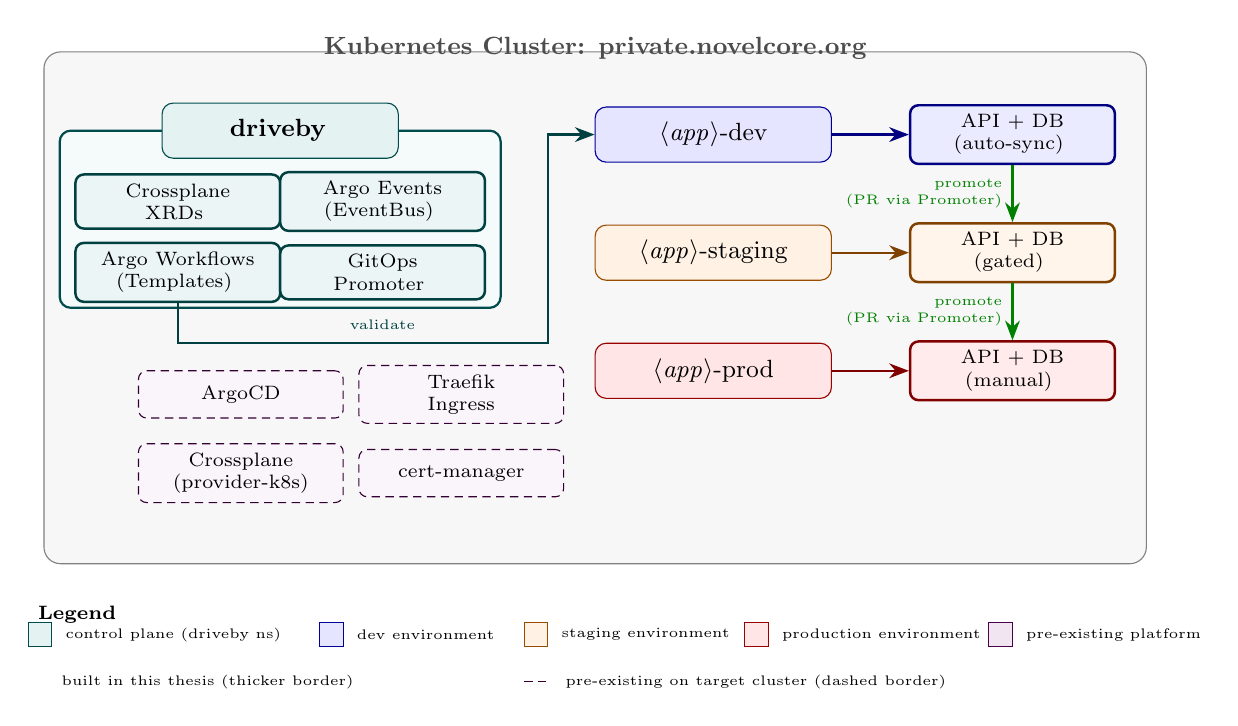
\begin{tikzpicture}[
    >={Stealth[length=2.5mm]},
    node distance=0.8cm,
    ns/.style={
        rectangle,
        rounded corners=4pt,
        draw=#1!60!black,
        fill=#1!10,
        minimum width=3cm,
        minimum height=0.7cm,
        font=\small,
        align=center
    },
    component/.style={
        rectangle,
        rounded corners=3pt,
        draw=#1!50!black,
        fill=#1!8,
        minimum width=2.6cm,
        minimum height=0.6cm,
        font=\scriptsize,
        align=center
    },
    % "thesis-built" components are drawn with a thicker border and a small
    % star marker; pre-existing infrastructure uses a thin border.
    new/.style={
        rectangle,
        rounded corners=3pt,
        draw=#1!50!black,
        line width=0.9pt,
        fill=#1!8,
        minimum width=2.6cm,
        minimum height=0.6cm,
        font=\scriptsize,
        align=center
    },
    existing/.style={
        rectangle,
        rounded corners=3pt,
        draw=#1!40!black,
        densely dashed,
        fill=#1!4,
        minimum width=2.6cm,
        minimum height=0.6cm,
        font=\scriptsize,
        align=center
    },
    cluster/.style={
        rectangle,
        rounded corners=6pt,
        draw=black!50,
        fill=black!3,
        minimum width=14cm,
        minimum height=6.5cm
    },
    clabel/.style={
        font=\small\bfseries,
        text=black!70
    }
]

% Cluster boundary
\node[cluster] (cluster) at (6.5,-2.8) {};
\node[clabel] (clusterlabel) at (6.5,0.5) {Kubernetes Cluster: private.novelcore.org};

% Control Plane namespace (left) — thesis-built artifacts live here.
% Containment is drawn as a namespace box (no ns->component arrows; the
% previous fan arrows passed behind the component nodes — comment [216]).
\draw[teal!60!black, rounded corners=4pt, thick, fill=teal!4]
    (-0.3,-2.8) rectangle (5.3,-0.55);
\node[ns=teal] (driveby-ns) at (2.5,-0.55) {\textbf{driveby}\,$\bigstar$};
\node[new=teal] (xrds) at (1.2,-1.45) {Crossplane\\XRDs $\bigstar$};
\node[new=teal] (argo-events) at (3.8,-1.45) {Argo Events\\(EventBus) $\bigstar$};
\node[new=teal] (workflows) at (1.2,-2.35) {Argo Workflows\\(Templates) $\bigstar$};
\node[new=teal] (promoter) at (3.8,-2.35) {GitOps\\Promoter $\bigstar$};

% Application namespaces (right region) — generated per-app by XSDLC.
% One row per environment: namespace box (left) hosts the app box (right),
% so no namespace-to-app arrow crosses another environment's nodes.
% Labels are generic <app>-{dev,staging,prod}; the PoC used perfect-api.
\node[ns=blue]   (dev-ns)     at (8.0,-0.6) {$\langle$\textit{app}$\rangle$-dev};
\node[ns=orange] (staging-ns) at (8.0,-2.1) {$\langle$\textit{app}$\rangle$-staging};
\node[ns=red]    (prod-ns)    at (8.0,-3.6) {$\langle$\textit{app}$\rangle$-prod};

\node[new=blue]   (dev-app)  at (11.8,-0.6) {API + DB\\(auto-sync) $\bigstar$};
\node[new=orange] (stg-app)  at (11.8,-2.1) {API + DB\\(gated) $\bigstar$};
\node[new=red]    (prod-app) at (11.8,-3.6) {API + DB\\(manual) $\bigstar$};

\draw[->,thick,blue!50!black]   (dev-ns.east)     -- (dev-app.west);
\draw[->,thick,orange!50!black] (staging-ns.east) -- (stg-app.west);
\draw[->,thick,red!50!black]    (prod-ns.east)    -- (prod-app.west);

% Shared infrastructure (bottom left) — pre-existing on the target cluster
\node[existing=violet] (argocd)     at (2.0,-3.9) {ArgoCD};
\node[existing=violet] (crossplane) at (2.0,-4.9) {Crossplane\\(provider-k8s)};
\node[existing=violet] (traefik)    at (4.8,-3.9) {Traefik\\Ingress};
\node[existing=violet] (cert-mgr)   at (4.8,-4.9) {cert-manager};

% Promotion arrows — solid (consistent with the GitOps pipeline figure).
% Promotion is not a direct environment-to-environment transfer: the GitOps
% Promoter opens/merges a promotion PR for each transition, hence the label.
\draw[->,thick,green!50!black] (dev-app.south)
    -- node[left,font=\tiny,green!50!black,align=right]
       {promote\\(PR via Promoter)} (stg-app.north);
\draw[->,thick,green!50!black] (stg-app.south)
    -- node[left,font=\tiny,green!50!black,align=right]
       {promote\\(PR via Promoter)} (prod-app.north);

% Validation arrow — Argo Workflows validates the source (dev) environment.
% Routed orthogonally through the free channel between the control-plane
% box and the environment rows so it never passes behind a node.
\draw[->,thick,teal!50!black]
    (workflows.south) -- (1.2,-3.25) -- (5.9,-3.25) -- (5.9,-0.6) -- (dev-ns.west);
\node[font=\tiny,teal!50!black,anchor=south] at (3.8,-3.2) {validate};

% ==================== Legend ====================
% Colour semantics + "existing vs thesis-built" key per comments [337], [338].
% Positioned below the cluster boundary (cluster bottom ~y=-6.05 so legend
% starts at y=-6.7 to leave a clear margin and avoid frame overlap).
\node[anchor=west, font=\scriptsize\bfseries] at (-0.7,-6.7) {Legend};

% Colour band
\fill[teal!10,draw=teal!60!black]   (-0.7,-7.1) rectangle (-0.4,-6.8);
\node[anchor=west, font=\tiny] at (-0.35,-6.95) {control plane (driveby ns)};

\fill[blue!10,draw=blue!60!black]   (3.0,-7.1) rectangle (3.3,-6.8);
\node[anchor=west, font=\tiny] at (3.35,-6.95) {dev environment};

\fill[orange!10,draw=orange!60!black] (5.6,-7.1) rectangle (5.9,-6.8);
\node[anchor=west, font=\tiny] at (5.95,-6.95) {staging environment};

\fill[red!10,draw=red!60!black]     (8.4,-7.1) rectangle (8.7,-6.8);
\node[anchor=west, font=\tiny] at (8.75,-6.95) {production environment};

\fill[violet!10,draw=violet!60!black] (11.5,-7.1) rectangle (11.8,-6.8);
\node[anchor=west, font=\tiny] at (11.85,-6.95) {pre-existing platform};

% Existing vs new band
\node[anchor=west, font=\tiny\bfseries] at (-0.7,-7.55) {$\bigstar$};
\node[anchor=west, font=\tiny] at (-0.4,-7.55) {built in this thesis (thicker border)};

\draw[densely dashed, draw=violet!40!black] (5.6,-7.55) -- (5.95,-7.55);
\node[anchor=west, font=\tiny] at (6.0,-7.55) {pre-existing on target cluster (dashed border)};

\end{tikzpicture}
%
}
\caption{System context showing the DriveBy control plane namespace, application environment namespaces, and shared infrastructure components. Dashed arrows indicate promotion flow and validation direction.}
\label{fig:k8s-system-context}
\end{figure}

The namespace layout enforces isolation. The \texttt{driveby} namespace owns the quality gate infrastructure: Crossplane XRDs and compositions, Argo Events resources (EventBus, EventSource, Sensor), workflow templates, and GitOps Promoter resources. Application namespaces own the API deployments and their databases. Validation workflows run in the \texttt{driveby} namespace but reach into application namespaces to access API endpoints, ensuring that the quality gate infrastructure does not require elevated permissions in application namespaces.

Shared infrastructure---ArgoCD, Crossplane with \texttt{provider-kubernetes}~v0.14.1, Traefik for ingress, and cert-manager for TLS---is pre-installed and managed by the platform team. The DriveBy Helm chart does not install these prerequisites; it \textit{references} them. An Ingress resource references the Traefik ingress class. A certificate annotation references the cert-manager issuer. An EventBus references the NATS JetStream substrate. None of these references are static configuration that a developer writes by hand---they are inherited capabilities provided by the platform, analogous to how an object in an object-oriented program inherits methods from its superclass without reimplementing them. This thesis, by design, shows only the ``application layer'' of an internal developer platform: the small, declarative surface that an API team interacts with. Everything beneath---the ingress routing, the certificate lifecycle, the event transport, the Git reconciliation---is the platform's responsibility, inherited through Kubernetes resource references.

% ============================================================================
\section{Crossplane XRD Design}
\label{sec:xrd-design}
% ============================================================================

The quality gate infrastructure is provisioned through two Crossplane Composite Resource Definitions (XRDs): \texttt{XQualityGateTemplate} for shared resources and \texttt{XQualityGate} for per-API resources. This two-XRD model separates concerns that change at different rates.

% ----------------------------------------------------------------------------
\subsection{XQualityGateTemplate: Shared Infrastructure}
\label{subsec:xrd-template}
% ----------------------------------------------------------------------------

The \texttt{XQualityGateTemplate} (API group \texttt{driveby.io/v1alpha1}) declares the validation workflow shared across all APIs monitored by a given quality gate. A single template instance generates four Kubernetes resources:

\begin{enumerate}
    \item A \textbf{ServiceAccount} with image pull credentials for accessing the DriveBy container image from the GitHub Container Registry.
    \item A \textbf{Role} granting permissions to create and manage Argo Workflows, read secrets and configmaps, manage persistent volume claims, and---when the GitOps Promoter is enabled---create and update CommitStatus custom resources.
    \item A \textbf{RoleBinding} associating the service account with the role.
    \item A \textbf{WorkflowTemplate} containing the seven-step validation DAG described in Section~\ref{sec:argo-workflows-dag}.
\end{enumerate}

The template's spec accepts configuration for the project name, gate name, target cluster, validation mode (minimal, strict, or test-only), secret references, and optional GitOps Promoter integration. These values are resolved through the three-tier configuration model described in Section~\ref{sec:three-tier-config} and injected into the generated resources via go-templating.

Listing~\ref{lst:template-cr} shows a representative \texttt{XQualityGateTemplate} instance.

\begin{lstlisting}[caption={XQualityGateTemplate custom resource.},label={lst:template-cr}]
apiVersion: driveby.io/v1alpha1
kind: XQualityGateTemplate
metadata:
  name: driveby-staging-promotion
spec:
  projectName: driveby
  gateName: staging-promotion
  gateKey: driveby/staging-promotion
  validationConfig:
    validationMode: strict
  promoterConfig:
    enabled: true
\end{lstlisting}

From this declaration, Crossplane generates the RBAC resources and a WorkflowTemplate with all seven validation steps, parameter definitions, and exit handlers. The operator writes six lines of meaningful configuration; the composition generates several hundred lines of Kubernetes manifests.

% ----------------------------------------------------------------------------
\subsection{XQualityGate: Per-API Event Pipeline}
\label{subsec:xrd-instance}
% ----------------------------------------------------------------------------

The \texttt{XQualityGate} (API group \texttt{driveby.io/v1alpha1}) declares the event-driven pipeline for a specific API. Each instance references a template (via \texttt{templateRef}) and generates the resources needed to receive events, filter them, and submit workflow runs. A single instance generates up to eight resources:

\begin{enumerate}
    \item An \textbf{EventBus} backed by NATS JetStream~\cite{nats-jetstream} for reliable event delivery between EventSource and Sensor.
    \item An \textbf{EventSource} configured as a webhook listener on a configurable port (default: 12000).
    \item A \textbf{Sensor} that filters events (e.g., only \texttt{pull\_request} events with actions \texttt{opened}, \texttt{reopened}, or \texttt{synchronize}) and submits workflow runs with extracted parameters.
    \item A \textbf{Service} exposing the EventSource webhook.
    \item An \textbf{Ingress} with TLS termination (via cert-manager) routing external webhook traffic to the EventSource service.
\end{enumerate}

When the GitOps Promoter is enabled, three additional resources are generated:

\begin{enumerate}
    \setcounter{enumi}{5}
    \item A \textbf{ScmProvider} authenticating to GitHub via a GitHub App.
    \item A \textbf{GitRepository} pointing to the GitOps repository.
    \item A \textbf{PromotionStrategy} defining the environment chain (e.g., dev $\rightarrow$ staging $\rightarrow$ prod) with per-environment auto-merge policies and commit status gates.
\end{enumerate}

Figure~\ref{fig:xrd-resource-hierarchy} visualizes the resource hierarchy generated by each XRD.

\begin{figure}[htbp]
\centering
% XSDLC Resource Hierarchy — Chapter 5
% Shows: Single XSDLC CR generating app-level, per-environment, and per-gate
% resources (three groups, matching the figure caption).
% Updated 2026-06 (round-2 review):
%   [234] arrows render completely — nodes are spaced 0.9cm apart (0.3cm gap
%         between borders > 2.5mm arrowhead) and every arrow is anchored on
%         node boundaries.
%   [235] added the Per-environment group (PromotionStrategy, Branches,
%         overlay RepositoryFile, ghcr-creds, ArgoCD Application) so the
%         figure agrees with the caption's three resource groups.
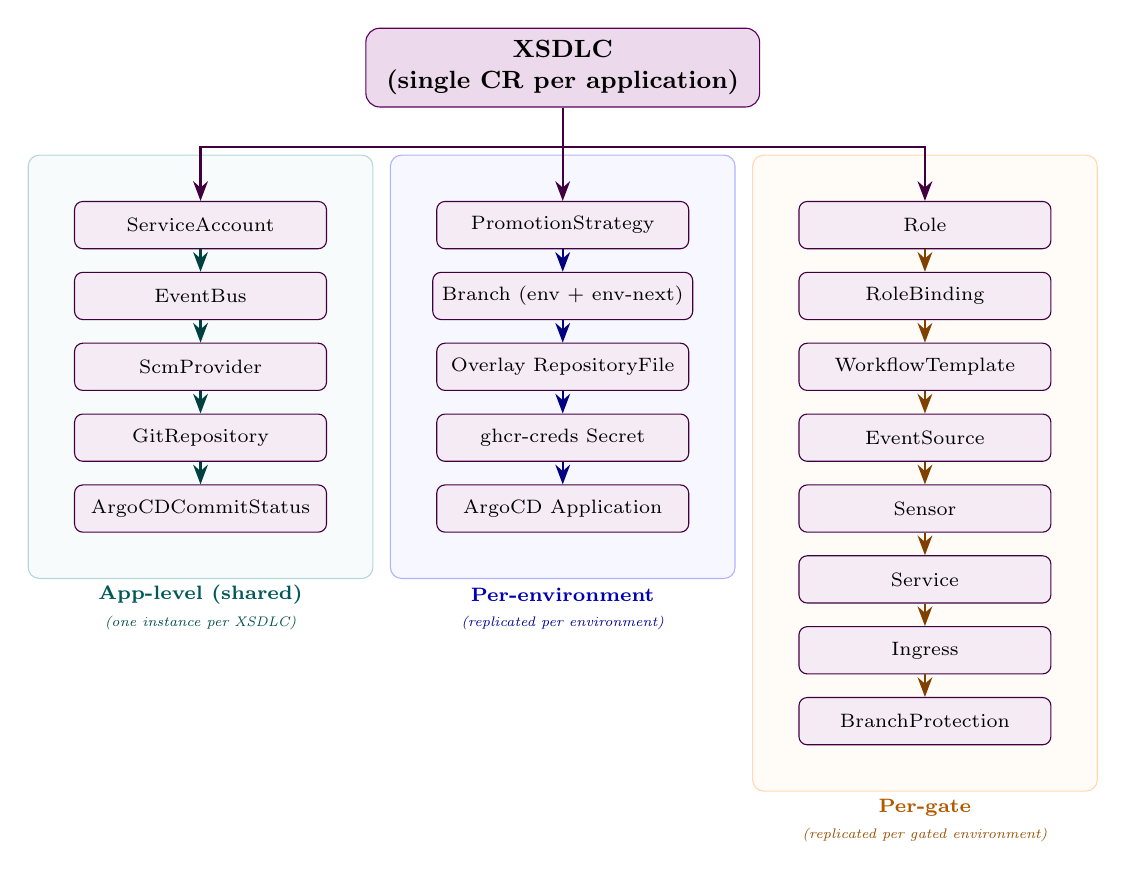
\begin{tikzpicture}[
    >={Stealth[length=2.5mm]},
    node distance=0.7cm,
    xrd/.style={
        rectangle,
        rounded corners=5pt,
        draw=violet!70!black,
        fill=violet!15,
        minimum width=5cm,
        minimum height=1cm,
        font=\small\bfseries,
        align=center
    },
    resource/.style={
        rectangle,
        rounded corners=3pt,
        draw=violet!50!black,
        fill=violet!8,
        minimum width=3.2cm,
        minimum height=0.6cm,
        font=\scriptsize,
        align=center
    },
    group/.style={
        rectangle,
        rounded corners=4pt,
        draw=#1!30,
        fill=#1!3,
        inner sep=8pt
    },
    grouplabel/.style={
        font=\scriptsize\bfseries,
        text=#1!70!black
    }
]

% XSDLC CR at top
\node[xrd] (xsdlc) at (4.6,0) {XSDLC\\(single CR per application)};

% --- App-level resources (left column) ---
\node[resource] (sa)       at (0,-2.0) {ServiceAccount};
\node[resource] (eb)       at (0,-2.9) {EventBus};
\node[resource] (scm)      at (0,-3.8) {ScmProvider};
\node[resource] (gitrepo)  at (0,-4.7) {GitRepository};
\node[resource] (commitst) at (0,-5.6) {ArgoCDCommitStatus};

\begin{scope}[on background layer]
    \node[group=teal, fit={($(sa.north west)+(-0.3,0.3)$) ($(commitst.south east)+(0.3,-0.3)$)}] (appgrp) {};
\end{scope}

% --- Per-environment resources (middle column) ---
\node[resource] (promstrat) at (4.6,-2.0) {PromotionStrategy};
\node[resource] (branch)    at (4.6,-2.9) {Branch (env + env-next)};
\node[resource] (overlay)   at (4.6,-3.8) {Overlay RepositoryFile};
\node[resource] (ghcr)      at (4.6,-4.7) {ghcr-creds Secret};
\node[resource] (argoapp)   at (4.6,-5.6) {ArgoCD Application};

\begin{scope}[on background layer]
    \node[group=blue, fit={($(promstrat.north west)+(-0.3,0.3)$) ($(argoapp.south east)+(0.3,-0.3)$)}] (envgrp) {};
\end{scope}

% --- Per-gate resources (right column) ---
\node[resource] (role)    at (9.2,-2.0) {Role};
\node[resource] (rb)      at (9.2,-2.9) {RoleBinding};
\node[resource] (wft)     at (9.2,-3.8) {WorkflowTemplate};
\node[resource] (es)      at (9.2,-4.7) {EventSource};
\node[resource] (sensor)  at (9.2,-5.6) {Sensor};
\node[resource] (svc)     at (9.2,-6.5) {Service};
\node[resource] (ing)     at (9.2,-7.4) {Ingress};
\node[resource] (bp)      at (9.2,-8.3) {BranchProtection};

\begin{scope}[on background layer]
    \node[group=orange, fit={($(role.north west)+(-0.3,0.3)$) ($(bp.south east)+(0.3,-0.3)$)}] (gategrp) {};
\end{scope}

% Arrows from XSDLC to the three groups (anchored on node boundaries)
\draw[->,thick,violet!50!black] (xsdlc.south) -- ++(0,-0.5) -| (sa.north);
\draw[->,thick,violet!50!black] (xsdlc.south) -- (promstrat.north);
\draw[->,thick,violet!50!black] (xsdlc.south) -- ++(0,-0.5) -| (role.north);

% Chained arrows inside each group (border-to-border, 0.3cm gaps)
\draw[->,thick,teal!50!black] (sa.south) -- (eb.north);
\draw[->,thick,teal!50!black] (eb.south) -- (scm.north);
\draw[->,thick,teal!50!black] (scm.south) -- (gitrepo.north);
\draw[->,thick,teal!50!black] (gitrepo.south) -- (commitst.north);

\draw[->,thick,blue!50!black] (promstrat.south) -- (branch.north);
\draw[->,thick,blue!50!black] (branch.south) -- (overlay.north);
\draw[->,thick,blue!50!black] (overlay.south) -- (ghcr.north);
\draw[->,thick,blue!50!black] (ghcr.south) -- (argoapp.north);

\draw[->,thick,orange!50!black] (role.south) -- (rb.north);
\draw[->,thick,orange!50!black] (rb.south) -- (wft.north);
\draw[->,thick,orange!50!black] (wft.south) -- (es.north);
\draw[->,thick,orange!50!black] (es.south) -- (sensor.north);
\draw[->,thick,orange!50!black] (sensor.south) -- (svc.north);
\draw[->,thick,orange!50!black] (svc.south) -- (ing.north);
\draw[->,thick,orange!50!black] (ing.south) -- (bp.north);

% Group labels + cardinality, placed below each group (clear of all arrows)
\node[grouplabel=teal] at (0,-6.7) {App-level (shared)};
\node[font=\tiny\itshape,text=teal!60!black] at (0,-7.05) {(one instance per XSDLC)};

\node[grouplabel=blue] at (4.6,-6.7) {Per-environment};
\node[font=\tiny\itshape,text=blue!60!black] at (4.6,-7.05) {(replicated per environment)};

\node[grouplabel=orange] at (9.2,-9.4) {Per-gate};
\node[font=\tiny\itshape,text=orange!60!black] at (9.2,-9.75) {(replicated per gated environment)};

\end{tikzpicture}

\caption{Resources generated by each XRD. The template produces shared RBAC and workflow infrastructure; the instance produces per-API event routing and optional GitOps Promoter resources. The \texttt{templateRef} link connects instances to their shared template.}
\label{fig:xrd-resource-hierarchy}
\end{figure}

The two-XRD model enables a one-to-many relationship: a single \texttt{XQualityGateTemplate} defines the validation pipeline once, and multiple \texttt{XQualityGate} instances---one per API---share that pipeline while maintaining independent event sources, sensors, and ingress routes. Adding a new API to the quality gate requires creating one \texttt{XQualityGate} custom resource; the shared template needs no modification.

The analogy to object-oriented programming is direct. The \texttt{XQualityGateTemplate} is a class definition: it encapsulates the validation behavior (WorkflowTemplate), the permissions model (RBAC), and the execution identity (ServiceAccount). The \texttt{XQualityGate} is an object instantiation: it provides instance-specific state (which API, which events, which namespaces) while inheriting all behavior from the template via \texttt{templateRef}. The platform infrastructure beneath both---Crossplane, Argo Events, cert-manager, Traefik---is the runtime: it provides the capabilities that make instantiation possible but is never configured by the application developer. Writing \texttt{kind: XQualityGate} is the Kubernetes equivalent of \texttt{Dog d = new Dog()}: a single declaration that activates an entire inheritance hierarchy of platform capabilities.

% ============================================================================
\section{Composition Pipeline}
\label{sec:composition-pipeline}
% ============================================================================

% ----------------------------------------------------------------------------
\subsection{Pipeline-Mode Compositions}
\label{subsec:pipeline-mode}
% ----------------------------------------------------------------------------

Both XRDs use Crossplane's pipeline-mode compositions, which process the composite resource through a sequence of functions rather than relying on the legacy patch-and-transform approach. The composition pipeline for each XRD follows the same four-step pattern:

\begin{enumerate}
    \item \textbf{function-environment-configs}: Injects cluster-level configuration from Crossplane EnvironmentConfig resources into the composition context. This is the second tier of the three-tier configuration model.
    \item \textbf{function-go-templating}: Renders Kubernetes manifests from Go templates, with access to the XRD spec, EnvironmentConfig data, and Helm-injected defaults.
    \item \textbf{function-auto-ready}: Automatically marks the composite resource as ready when all composed resources reach their ready state.
    \item \textbf{function-sequencer}: Controls the order in which composed resources are created, preventing race conditions (e.g., ensuring the EventBus exists before the Sensor that depends on it).
\end{enumerate}

The go-templating function performs the bulk of the work. It evaluates conditional blocks (e.g., generating GitOps Promoter resources only when \texttt{promoterConfig.enabled} is true), resolves the three-tier configuration precedence, and handles the template escaping required when generating Argo Workflows templates that themselves contain Go template syntax.

% ----------------------------------------------------------------------------
\subsection{Template Escaping}
\label{subsec:template-escaping}
% ----------------------------------------------------------------------------

A notable engineering challenge arises from the nested templating layers. The Crossplane composition uses Go templates to generate Argo Workflows manifests, which themselves use Go template syntax for parameter substitution (e.g., \texttt{\{\{workflow.parameters.app-name\}\}}). Without escaping, the Crossplane go-templating function would attempt to evaluate the Argo template expressions during composition rendering, causing failures.

The solution uses a double-escaping convention. Argo template expressions within the composition are written as:

\begin{verbatim}
{{ "{{" }}workflow.parameters.app-name{{ "}}" }}
\end{verbatim}

The outer Go template evaluates \texttt{\{\{"{{"\}\}} to produce the literal string \texttt{\{\{}, and similarly for the closing braces. The resulting manifest contains the intended Argo expression \texttt{\{\{workflow.parameters.app-name\}\}} verbatim. This escaping is applied consistently across all workflow step definitions in the template composition.

% ============================================================================
\section{Three-Tier Configuration Model}
\label{sec:three-tier-config}
% ============================================================================

The system implements a three-tier configuration resolution model that balances simplicity with flexibility. Figure~\ref{fig:three-tier-config} illustrates the resolution order.

\begin{figure}[htbp]
\centering
% Three-Tier Configuration Resolution — Chapter 5
% Shows: Helm defaults → EnvironmentConfig → XRD spec (with override arrows)
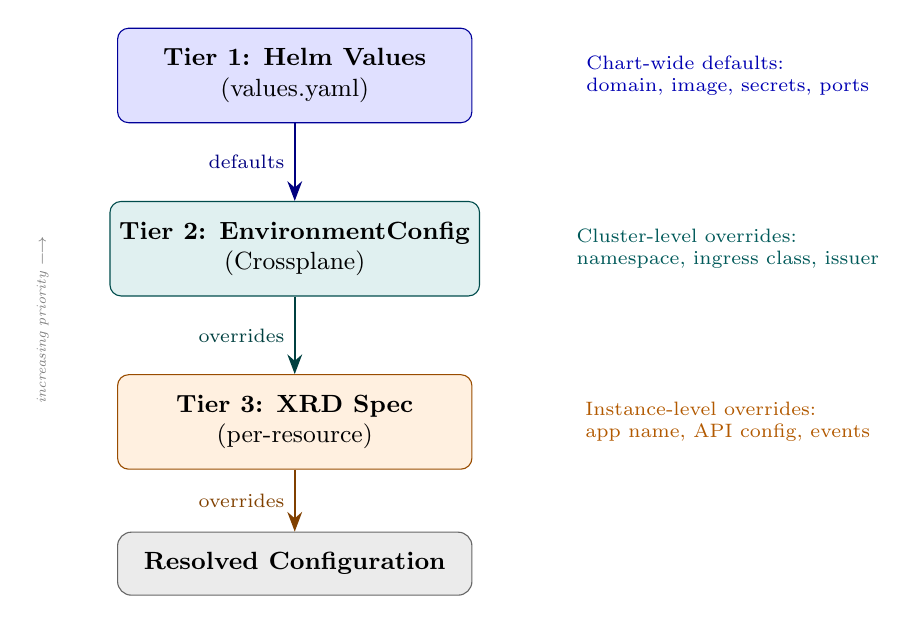
\begin{tikzpicture}[
    >={Stealth[length=2.5mm]},
    node distance=1.2cm,
    tier/.style={
        rectangle,
        rounded corners=4pt,
        draw=#1!60!black,
        fill=#1!12,
        minimum width=4.5cm,
        minimum height=1.2cm,
        font=\small,
        align=center
    },
    desc/.style={
        font=\scriptsize,
        text=#1!70!black,
        align=left
    },
    result/.style={
        rectangle,
        rounded corners=5pt,
        draw=black!60,
        fill=black!8,
        minimum width=4.5cm,
        minimum height=0.8cm,
        font=\small\bfseries,
        align=center
    },
    override/.style={
        ->,
        thick,
        #1!50!black
    }
]

% Three tiers (top to bottom = lowest to highest priority)
\node[tier=blue] (helm) at (0,0) {\textbf{Tier 1: Helm Values}\\(values.yaml)};
\node[desc=blue] at (5.5,0) {Chart-wide defaults:\\domain, image, secrets, ports};

\node[tier=teal] (envconfig) at (0,-2.2) {\textbf{Tier 2: EnvironmentConfig}\\(Crossplane)};
\node[desc=teal] at (5.5,-2.2) {Cluster-level overrides:\\namespace, ingress class, issuer};

\node[tier=orange] (xrd) at (0,-4.4) {\textbf{Tier 3: XRD Spec}\\(per-resource)};
\node[desc=orange] at (5.5,-4.4) {Instance-level overrides:\\app name, API config, events};

\node[result] (resolved) at (0,-6.2) {Resolved Configuration};

% Override arrows (each tier overrides the previous)
\draw[override=blue] (helm) -- node[left,font=\scriptsize] {defaults} (envconfig);
\draw[override=teal] (envconfig) -- node[left,font=\scriptsize] {overrides} (xrd);
\draw[override=orange] (xrd) -- node[left,font=\scriptsize] {overrides} (resolved);

% Priority label
\node[font=\tiny\itshape,rotate=90,text=black!50] at (-3.2,-3.1) {increasing priority $\longrightarrow$};

\end{tikzpicture}

\caption{Three-tier configuration resolution. Each tier overrides values from the tier above, with Tier~3 (XRD spec) having the highest priority.}
\label{fig:three-tier-config}
\end{figure}

\textbf{Tier~1: Helm values} (\texttt{values.yaml}) provide chart-wide defaults that apply to all resources generated by the Helm chart. These include the base domain (\texttt{private.novelcore.org}), the DriveBy container image (\texttt{ghcr.io/meter-peter/driveby:latest}), secret names, webhook port (12000), EventBus configuration, and ingress settings. Tier~1 values are baked into the composition templates at Helm rendering time.

\textbf{Tier~2: EnvironmentConfigs} provide cluster-level overrides that take precedence over Helm defaults. Two EnvironmentConfigs are deployed: \texttt{driveby-template-config} (shared defaults for template compositions) and \texttt{driveby-instance-config} (defaults for instance compositions). These are Crossplane-native resources that can be updated independently of the Helm chart, enabling per-cluster customization without chart modifications.

\textbf{Tier~3: XRD spec fields} provide per-resource overrides with the highest priority. When an operator specifies a value in the \texttt{XQualityGateTemplate} or \texttt{XQualityGate} spec, it takes precedence over both EnvironmentConfig and Helm defaults. This tier enables per-API customization (e.g., a specific API using a different validation mode or a non-standard port).

The resolution is implemented in the go-templating function using a precedence chain. For each configurable value, the template checks: (1)~if the XRD spec provides the value, use it; (2)~else if the EnvironmentConfig provides the value, use it; (3)~else use the Helm default. This pattern is applied consistently across more than twenty configurable parameters including domain, namespace, image references, secret names, ingress class, cluster issuer, webhook port, JetStream version and replicas, and GitHub configuration.

Table~\ref{tab:config-tiers} lists representative parameters and their resolution across tiers.

\begin{table}[htbp]
\centering
\caption{Representative configuration parameters and their three-tier resolution.}
\label{tab:config-tiers}
\small
\begin{tabular}{@{}llll@{}}
\toprule
\textbf{Parameter} & \textbf{Tier~1 (Helm)} & \textbf{Tier~2 (EnvConfig)} & \textbf{Tier~3 (XRD)} \\
\midrule
Base domain        & \texttt{private.novelcore.org} & --- & --- \\
DriveBy image      & \texttt{ghcr.io/.../driveby:latest} & --- & per-resource \\
Validation mode    & \texttt{strict} & --- & per-resource \\
Webhook port       & 12000 & per-cluster & per-resource \\
Ingress class      & \texttt{traefik-system} & per-cluster & --- \\
JetStream replicas & 1 & per-cluster & per-resource \\
GitHub API URL     & \texttt{https://api.github.com} & per-cluster & --- \\
\bottomrule
\end{tabular}
\end{table}

% ============================================================================
\section{Argo Events Architecture}
\label{sec:argo-events-arch}
% ============================================================================

Argo Events provides the event-driven layer that connects external triggers (GitHub webhooks) to internal actions (workflow submissions). The architecture uses three Argo Events resources, each generated by the \texttt{XQualityGate} composition.

% ----------------------------------------------------------------------------
\subsection{EventBus}
\label{subsec:eventbus}
% ----------------------------------------------------------------------------

The EventBus is the message transport layer between EventSources and Sensors. It is backed by NATS JetStream~\cite{nats-jetstream}, which provides persistent, at-least-once delivery semantics. The EventBus must be named \texttt{default} within each namespace (an Argo Events convention) and is configured with a single replica for the development deployment, though production deployments would scale to three replicas for high availability.

The JetStream backing ensures that webhook events are not lost if the Sensor is temporarily unavailable. Events are persisted to the JetStream stream and replayed when the Sensor reconnects, providing reliability without requiring external message queue infrastructure.

% ----------------------------------------------------------------------------
\subsection{EventSource}
\label{subsec:eventsource}
% ----------------------------------------------------------------------------

The EventSource defines how external events enter the system. For quality gate validation, the EventSource is configured as a webhook listener on port 12000. Each event trigger defined in the \texttt{XQualityGate} spec generates a named webhook endpoint. For example, a trigger named \texttt{pr-validation} produces an endpoint at:

\begin{verbatim}
/perfect-api-staging-promotion-pr-validation
\end{verbatim}

GitHub is configured to deliver webhook events to this endpoint via the Ingress route. The EventSource receives the raw webhook payload, validates it, and publishes it to the EventBus for consumption by Sensors.

% ----------------------------------------------------------------------------
\subsection{Sensor and Parameter Extraction}
\label{subsec:sensor}
% ----------------------------------------------------------------------------

The Sensor subscribes to events from the EventBus, applies filtering logic, and triggers workflow submissions when filter conditions are met. For pull request validation, the Sensor filters on:

\begin{itemize}
    \item Event type: \texttt{pull\_request}
    \item Action: \texttt{opened}, \texttt{reopened}, or \texttt{synchronize}
\end{itemize}

This filtering ensures that workflows are triggered only for meaningful PR events---new PRs, reopened PRs, or new commits pushed to existing PRs---and not for label changes, review requests, or other non-code events.

When a matching event arrives, the Sensor extracts parameters from the webhook payload using JSONPath expressions and passes them to the workflow submission. Table~\ref{tab:sensor-params} lists the extracted parameters.

\begin{table}[htbp]
\centering
\caption{Parameters extracted from webhook payload by the Sensor.}
\label{tab:sensor-params}
\small
\begin{tabular}{@{}lll@{}}
\toprule
\textbf{Parameter} & \textbf{JSONPath Source} & \textbf{Purpose} \\
\midrule
\texttt{app-name}         & XRD spec (static)                    & Identifies the API being validated \\
\texttt{pr-number}        & \texttt{body.number}                 & PR comment and status reporting \\
\texttt{head-sha}         & \texttt{body.pull\_request.head.sha} & Commit status target \\
\texttt{github-owner}     & \texttt{body.repository.owner.login} & GitHub API calls \\
\texttt{github-repo}      & \texttt{body.repository.name}        & GitHub API calls \\
\texttt{source-namespace} & XRD spec (static)                    & Environment to validate against \\
\texttt{target-namespace} & XRD spec (static)                    & Promotion target \\
\texttt{service-name}     & XRD spec (static)                    & Kubernetes service to validate \\
\texttt{openapi-endpoint} & XRD spec (default: \texttt{/openapi.json}) & Spec URL path \\
\texttt{app-port}         & XRD spec (default: 8000)             & Service port \\
\bottomrule
\end{tabular}
\end{table}

The parameter extraction combines dynamic values from the webhook payload (PR number, commit SHA, repository details) with static values from the XRD spec (app name, namespaces, service configuration). This hybrid approach enables the workflow to operate on the specific PR that triggered validation while targeting the correct application environment.

% ============================================================================
\section{Argo Workflows Validation DAG}
\label{sec:argo-workflows-dag}
% ============================================================================

The validation pipeline is implemented as an Argo Workflows WorkflowTemplate containing a directed acyclic graph (DAG) of seven steps. The Sensor submits workflow runs from this template, passing the extracted parameters. Figure~\ref{fig:staging-dag} (reproduced from Chapter~\ref{ch:architecture}) shows the DAG structure.

% ----------------------------------------------------------------------------
\subsection{Pipeline Steps}
\label{subsec:pipeline-steps}
% ----------------------------------------------------------------------------

The seven steps execute in the following order, with steps 6 and 7 running in parallel after step 5:

\textbf{Step 1: set-pending-status.} Posts a ``pending'' commit status to the PR's head SHA via the GitHub API. This provides immediate visual feedback on the PR that validation is in progress. When the GitOps Promoter is enabled, a parallel step creates a CommitStatus custom resource with phase \texttt{pending}.

\textbf{Step 2: wait-for-source-ready.} Polls the source environment (e.g., \texttt{perfect-api-dev}) to verify that the API deployment is healthy and ready to accept validation requests. The step performs up to 24 health checks at 5-second intervals (2 minutes maximum), using \texttt{curl} to probe the API's health endpoint. This wait ensures that validation does not run against a partially deployed or restarting instance.

\textbf{Step 3: spec-sync-check.} Fetches the OpenAPI specification from the source environment's API endpoint and verifies it is accessible. This step detects configuration errors (wrong port, wrong endpoint path, service not exposed) before the main validation begins.

\textbf{Step 4: validate-source.} Runs the DriveBy CLI in \texttt{validate-only} mode against the source environment's API. The container image \texttt{ghcr.io/meter-peter/driveby:latest} executes with the validation mode configured in the template (default: strict). The validation report is stored as a workflow artifact.

\textbf{Step 5: functional-test-source.} Runs the DriveBy CLI in \texttt{function-only} mode, executing functional tests against the live API instance in the source environment. Authentication credentials are injected from Kubernetes secrets.

\textbf{Step 6: report-success.} Posts a ``success'' commit status to the PR's head SHA. When the GitOps Promoter is enabled, updates the CommitStatus custom resource to phase \texttt{success}, signaling that the promotion gate has passed.

\textbf{Step 7: comment-pr.} Posts the validation report as a comment on the pull request using DriveBy's \texttt{--github-comment} flag. This provides human-readable results directly in the PR conversation.

% ----------------------------------------------------------------------------
\subsection{Exit Handler}
\label{subsec:exit-handler}
% ----------------------------------------------------------------------------

The workflow defines an exit handler that triggers on any step failure. The exit handler posts a ``failure'' commit status to the PR's head SHA, ensuring that the quality gate is explicitly closed even when validation fails. When the GitOps Promoter is enabled, the exit handler also updates the CommitStatus custom resource to phase \texttt{failure}, blocking automatic promotion.

The exit handler is critical for the quality gate pattern. Without it, a failed workflow would leave the commit status in ``pending'' state indefinitely, neither blocking nor approving promotion. The exit handler guarantees that every workflow run terminates with an explicit quality signal: success or failure, never ambiguous.

% ============================================================================
\section{Helm Chart Packaging}
\label{sec:helm-chart}
% ============================================================================

The entire Kubernetes infrastructure is packaged as a Helm chart (\texttt{driveby}, version~0.4.0) that installs all Crossplane resources, XRDs, compositions, and provider configuration in a single \texttt{helm install} command.

% ----------------------------------------------------------------------------
\subsection{Chart Structure and Install Order}
\label{subsec:chart-structure}
% ----------------------------------------------------------------------------

The chart contains Crossplane provider references (\texttt{provider-kubernetes}~v0.14.1), Crossplane functions (go-templating, auto-ready, sequencer, environment-configs), XRD definitions (template and instance), composition definitions (template and instance), a ProviderConfig for the Kubernetes provider, and optional secret templates.

Installation follows an eight-step order designed to handle Crossplane's CRD chicken-and-egg problem: the Crossplane provider must be installed and healthy before ProviderConfig resources that reference it, and XRDs must be installed before compositions that implement them. The recommended sequence is:

\begin{enumerate}
    \item Pre-install: Crossplane provider and functions (wait for CRDs)
    \item Secrets: GitHub PAT, API auth, image pull credentials
    \item Helm install: XRDs, compositions, ProviderConfig
    \item EnvironmentConfigs: Cluster-level configuration
    \item XQualityGateTemplate: Shared validation infrastructure
    \item XQualityGate: Per-API event pipeline
    \item GitHub webhook: Configure repository webhook to the Ingress endpoint
    \item GitOps Promoter: ScmProvider, GitRepository, PromotionStrategy (if enabled)
\end{enumerate}

Steps 5--8 are handled by Crossplane once the XRDs and compositions are installed. The operator creates the custom resources (steps 5--6) and Crossplane provisions all child resources automatically.

% ----------------------------------------------------------------------------
\subsection{OCI Distribution}
\label{subsec:oci-distribution}
% ----------------------------------------------------------------------------

The chart is published to an OCI-compliant registry~\cite{helm-oci} at \texttt{oci://ghcr.io/meter-peter/charts/driveby}. OCI distribution eliminates the need for a separate Helm chart repository; the chart is stored alongside the container images in the GitHub Container Registry. Installation uses standard Helm OCI syntax:

\begin{verbatim}
helm install driveby oci://ghcr.io/meter-peter/charts/driveby \
  --version 0.4.0 --namespace driveby --create-namespace
\end{verbatim}

Versioned chart releases are produced automatically by the release pipeline described in Chapter~\ref{ch:workflow}.

% ============================================================================
\section{Summary}
\label{sec:k8s-summary}
% ============================================================================

This chapter described the Kubernetes infrastructure that transforms DriveBy from a standalone CLI tool into a declarative, event-driven quality gate system. The two-XRD model (Section~\ref{sec:xrd-design}) separates shared validation logic from per-API event routing, enabling a one-to-many relationship between templates and instances. The composition pipeline (Section~\ref{sec:composition-pipeline}) uses Crossplane's pipeline-mode functions to generate all required resources from minimal operator input. The three-tier configuration model (Section~\ref{sec:three-tier-config}) balances simplicity with flexibility across chart, cluster, and resource levels.

The Argo Events layer (Section~\ref{sec:argo-events-arch}) provides reliable, filtered event delivery from GitHub webhooks to workflow submissions. The seven-step Argo Workflows DAG (Section~\ref{sec:argo-workflows-dag}) orchestrates the full validation pipeline---from health checking through static validation and functional testing to commit status reporting---with an exit handler that guarantees explicit quality signals on every run.

Chapter~\ref{ch:workflow} describes how this infrastructure operates within the broader GitOps pipeline: the promotion-driven quality gate flow, the GitOps Promoter's multi-environment model, and the CI/CD pipelines that build, test, and release the DriveBy system itself.

\chapter{GitOps Pipeline and CI/CD}
\label{ch:workflow}

Chapter~\ref{ch:kubernetes} described the Kubernetes infrastructure---Crossplane XRDs, Argo Events, Argo Workflows---that implements the quality gate system. This chapter describes how that infrastructure operates within the broader GitOps pipeline: the promotion-driven quality gate flow, the event-driven validation pipeline end-to-end, the single-repo architecture and its ``Bring Your Own CI'' design principle, the GitOps Promoter's multi-environment model, human-in-the-loop decision patterns, and the quality gate as a closed-loop control system. The chapter also describes the three CI/CD pipelines that build, test, and release the DriveBy system itself.

Together, Chapters~\ref{ch:architecture},~\ref{ch:kubernetes}, and this chapter form a three-layer value chain: the DriveBy CLI provides the validation logic, Kubernetes infrastructure orchestrates its execution, and GitOps pipelines make validation results drive promotion decisions. This chapter describes the outermost layer---the point where validation results become operational signals that advance or block software delivery.

The chapter addresses Research Question~3 (RQ3): \textit{How effectively does specification-driven quality assurance integrate into cloud-native GitOps pipelines as an autonomous quality gate?} The answer is demonstrated through a production deployment on the \texttt{private.novelcore.org} cluster, where DriveBy validates a reference API across three environments.

% ============================================================================
\section{Promotion-Driven Quality Gate}
\label{sec:promotion-driven-gate}
% ============================================================================

The quality gate operates on a key insight: \textit{validate the source environment, not the target}. When a developer merges code into the application repository, the CI pipeline builds and deploys the new version to the development environment. ArgoCD~\cite{argocd} synchronizes the development environment automatically. The GitOps Promoter detects the successful synchronization and creates a promotion pull request proposing to update the staging environment's manifest to the new version.

This promotion PR triggers the quality gate. The GitHub webhook fires, the EventSource receives the event, the Sensor filters for PR actions, and the Workflow executes validation against the \textit{development} environment---the environment where the new code is already running. The validation results determine whether the promotion PR is approved (merged) or blocked (left open with a failure status).

This inversion is deliberate. Validating the source environment ensures that quality is assessed against the actual deployment rather than a hypothetical future state. If the API in development passes strict DDT validation, the same code deployed to staging will behave identically (assuming equivalent infrastructure). The alternative---validating the target environment after promotion---would detect problems only after the potentially breaking change has already been deployed, violating the shift-left principle~\cite{shift-left}.

Figure~\ref{fig:gitops-pipeline} shows the end-to-end pipeline from developer pull request to validation feedback.

\begin{figure}[htbp]
\centering
\resizebox{\textwidth}{!}{%
% GitOps Event-Driven Pipeline with Source Hydrator — Chapter 6
% Developer commits dry manifests → Hydrator renders → -next branch → Promoter PR → Webhook → Argo Events → Workflow → Feedback
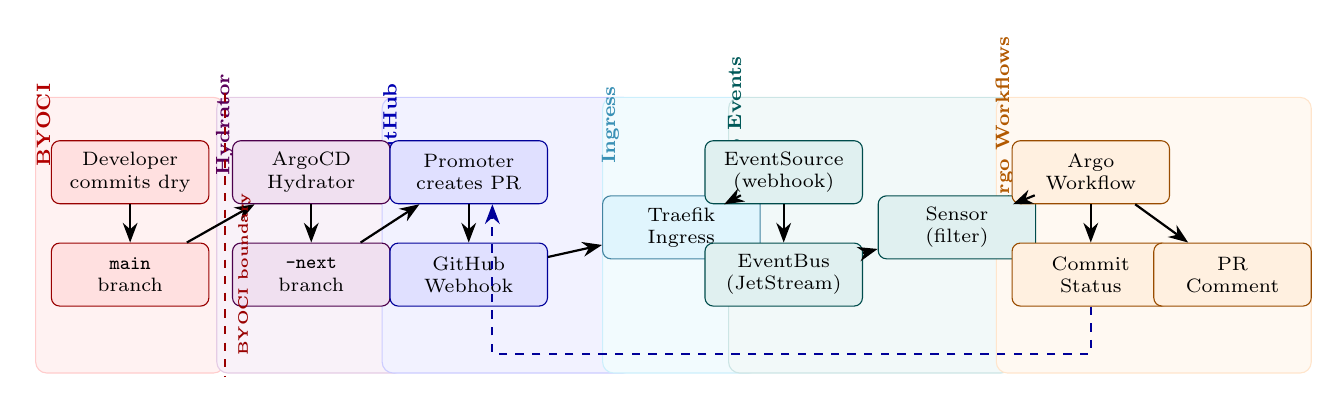
\begin{tikzpicture}[
    >={Stealth[length=2.5mm]},
    node distance=0.6cm,
    stage/.style={
        rectangle,
        rounded corners=3pt,
        draw=#1!60!black,
        fill=#1!12,
        minimum width=2cm,
        minimum height=0.8cm,
        font=\scriptsize,
        align=center
    },
    lane label/.style={
        font=\scriptsize\bfseries,
        rotate=90,
        anchor=center,
        text=#1!70!black
    },
    lane bg/.style={
        fill=#1!5,
        draw=#1!20,
        rounded corners=4pt
    }
]

% Lane backgrounds
\begin{scope}[on background layer]
    \node[lane bg=red,    minimum width=2.4cm, minimum height=3.5cm] at (-2,0) {};
    \node[lane bg=violet, minimum width=2.4cm, minimum height=3.5cm] at (0.3,0) {};
    \node[lane bg=blue,   minimum width=3.2cm, minimum height=3.5cm] at (2.8,0) {};
    \node[lane bg=cyan,   minimum width=2cm, minimum height=3.5cm] at (5,0) {};
    \node[lane bg=teal,   minimum width=3.6cm, minimum height=3.5cm] at (7.4,0) {};
    \node[lane bg=orange, minimum width=4cm, minimum height=3.5cm] at (11,0) {};
\end{scope}

% Lane labels (inside the lane background, near the top edge of each rectangle)
% Round-10 follow-up to supervisor [408]: previously sat outside the lane bg at y=1.9
% (above the rectangle); now positioned at y=1.4, inside each lane background
% (which extends from y=-1.75 to y=+1.75) above the top row of stages at y=0.8.
\node[lane label=red]     at (-3.1,1.4)  {BYOCI};
\node[lane label=violet]  at (-0.8,1.4)  {Hydrator};
\node[lane label=blue]    at (1.3,1.4)   {GitHub};
\node[lane label=cyan]    at (4.1,1.4)   {Ingress};
\node[lane label=teal]    at (5.7,1.4)   {Argo Events};
\node[lane label=orange]  at (9.1,1.4)   {Argo Workflows};

% BYOCI lane (developer trigger)
\node[stage=red] (deploy) at (-2,0.8)  {Developer\\commits dry};
\node[stage=red] (main)   at (-2,-0.5) {\texttt{main}\\branch};
\draw[->,thick] (deploy) -- (main);

% Hydrator lane
\node[stage=violet] (hydrator) at (0.3,0.8)  {ArgoCD\\Hydrator};
\node[stage=violet] (nextbr)   at (0.3,-0.5) {\texttt{-next}\\branch};
\draw[->,thick] (main) -- (hydrator);
\draw[->,thick] (hydrator) -- (nextbr);

% GitHub lane
\node[stage=blue] (promoter) at (2.3,0.8)  {Promoter\\creates PR};
\node[stage=blue] (webhook)  at (2.3,-0.5) {GitHub\\Webhook};
\draw[->,thick] (nextbr) -- (promoter);
\draw[->,thick] (promoter) -- (webhook);

% Ingress lane
\node[stage=cyan] (traefik) at (5,0.1) {Traefik\\Ingress};
\draw[->,thick] (webhook) -- (traefik);

% Argo Events lane
\node[stage=teal] (es)     at (6.3,0.8)  {EventSource\\(webhook)};
\node[stage=teal] (eb)     at (6.3,-0.5) {EventBus\\(JetStream)};
\node[stage=teal] (sensor) at (8.5,0.1)  {Sensor\\(filter)};
\draw[->,thick] (traefik) -- (es);
\draw[->,thick] (es) -- (eb);
\draw[->,thick] (eb) -- (sensor);

% Argo Workflows lane
\node[stage=orange] (wf)      at (10.2,0.8)  {Argo\\Workflow};
\node[stage=orange] (status)  at (10.2,-0.5) {Commit\\Status};
\node[stage=orange] (comment) at (12,-0.5)   {PR\\Comment};
\draw[->,thick] (sensor) -- (wf);
\draw[->,thick] (wf) -- (status);
\draw[->,thick] (wf) -- (comment);

% Feedback loop back to Promoter PR
\draw[->,thick,blue!60!black,dashed] (status.south) -- ++(0,-0.6) -| ($(promoter.south)+(0.3,-0.6)$) -- ($(promoter.south)+(0.3,0)$);

% BYOCI boundary annotation
\draw[dashed,thick,red!60!black] (-0.8,1.8) -- (-0.8,-1.8);
\node[font=\tiny\bfseries,text=red!60!black,anchor=north,rotate=90] at (-0.75,-0.5) {BYOCI boundary};

\end{tikzpicture}
%
}
\caption{End-to-end GitOps validation pipeline. A developer opens a promotion PR; the webhook triggers Argo Events, which submits an Argo Workflow. Validation results are posted back as commit status and PR comment (dashed feedback loop).}
\label{fig:gitops-pipeline}
\end{figure}

% ============================================================================
\section{Event-Driven Validation Pipeline}
\label{sec:event-pipeline-detail}
% ============================================================================

The event-driven pipeline transforms an external webhook into a structured validation workflow through five stages: ingress, event capture, event filtering, workflow submission, and feedback reporting. This section traces a single validation trigger through the entire pipeline.

% ----------------------------------------------------------------------------
\subsection{Webhook Delivery and Ingress}
\label{subsec:webhook-delivery}
% ----------------------------------------------------------------------------

The pipeline begins when GitHub delivers a webhook to the Ingress endpoint. The webhook URL follows the pattern:

\begin{verbatim}
https://{app}-{gate}-webhook.{domain}/{trigger-endpoint}
\end{verbatim}

For the reference deployment, this resolves to \texttt{https://perfect-api-staging-gate-webhook.private.novelcore.org/perfect-api-staging-gate-pr-trigger}. The Traefik Ingress controller terminates TLS (using a certificate issued by cert-manager), routes the request to the EventSource Service, and delivers the payload to the webhook listener on port~12000.

% ----------------------------------------------------------------------------
\subsection{Event Processing}
\label{subsec:event-processing}
% ----------------------------------------------------------------------------

The EventSource receives the webhook payload and publishes it to the EventBus (NATS JetStream). The Sensor subscribes to the EventBus and evaluates the event against its configured filters. For promotion PR validation, the Sensor checks that the event type is \texttt{pull\_request} and the action is one of \texttt{opened}, \texttt{reopened}, or \texttt{synchronize}. Events that do not match---such as PR label changes, review requests, or comment events---are silently discarded.

For matching events, the Sensor extracts ten parameters from the webhook payload using JSONPath expressions (detailed in Table~\ref{tab:sensor-params} of Chapter~\ref{ch:kubernetes}) and constructs a workflow submission request. The submission references the WorkflowTemplate generated by the \texttt{XSDLC} composition and passes the extracted parameters as workflow arguments.

% ----------------------------------------------------------------------------
\subsection{Latency Analysis}
\label{subsec:latency}
% ----------------------------------------------------------------------------

The end-to-end latency from webhook delivery to workflow completion depends on three factors: event processing overhead (typically under 2~seconds for EventSource $\rightarrow$ EventBus $\rightarrow$ Sensor $\rightarrow$ workflow submission), source readiness wait (0--120~seconds, depending on whether the deployment is already healthy), and validation execution time (10--60~seconds, depending on specification size and validation mode). In practice, a typical validation cycle for the reference API completes in under 90~seconds from PR creation to commit status posted.

% ============================================================================
\section{Single-Repo Architecture}
\label{sec:single-repo}
% ============================================================================

The quality gate system described in this thesis operates within a \textit{single-repository} model that deliberately separates application CI from platform-managed delivery. This section describes the architectural rationale, the boundary between developer and platform responsibilities, and the manifest propagation mechanism that bridges the two.

% ----------------------------------------------------------------------------
\subsection{Why a Single Repository}
\label{subsec:why-single-repo}
% ----------------------------------------------------------------------------

Traditional GitOps deployments maintain a separate \textit{config repository} alongside the application's source repository. The config repo holds Kubernetes manifests for each environment; a CI pipeline in the source repo updates the config repo on each build. This pattern doubles the number of repositories, fragments the change history across two Git logs, and introduces a synchronization pipeline (``update the config repo'') that must itself be maintained and monitored.

The XSDLC model eliminates this duplication. The application repository holds both source code and Kubernetes manifests in a single tree:

\begin{verbatim}
perfect-api/
  src/                     # Application source
  Dockerfile               # Build specification
  manifests/
    deployment.yaml        # Kubernetes deployment manifest
    service.yaml           # Kubernetes service manifest
\end{verbatim}

The developer maintains the manifests alongside the source code. When a CI pipeline builds a new container image, it updates \texttt{manifests/deployment.yaml} with the new image tag and pushes to \texttt{main}. The XSDLC delivery pipeline takes over from there, propagating manifests to environment branches, gating promotions, and syncing through ArgoCD. The developer never creates or manages environment branches, promotion PRs, or ArgoCD Applications---the XSDLC composition provisions all of these.

% ----------------------------------------------------------------------------
\subsection{Bring Your Own CI (BYOCI)}
\label{subsec:byoci}
% ----------------------------------------------------------------------------

The single-repo model embodies a deliberate design principle: \textbf{XSDLC owns delivery, not CI}. The boundary is explicit: \textit{XSDLC's responsibility begins when manifests land on \texttt{main}}.

Everything \textit{before} that boundary is the developer's responsibility: building the application, running unit tests, generating the container image, and updating the manifest with the new image tag. These tasks are inherently application-specific---a Python FastAPI service uses different build tools, test frameworks, and container patterns than a Go gRPC service. No platform abstraction can usefully generalize this diversity without either constraining developer choice or reimplementing CI functionality that mature tools (GitHub Actions, Jenkins, GitLab CI) already provide.

Everything \textit{after} that boundary is XSDLC's responsibility: propagating manifests to environment branches, triggering quality gates, managing promotion PRs, posting commit statuses, and syncing ArgoCD Applications. These tasks are platform-generic---the same propagation, gating, and promotion pattern applies regardless of the application's language, framework, or build tool.

This separation contrasts with opinionated CD platforms (Tekton Pipelines, Jenkins X) that attempt to own the full CI/CD lifecycle, providing build templates, test runners, and deployment strategies within a single framework. Such platforms trade flexibility for integration: they work well when the application fits their model and poorly when it does not. XSDLC is composable rather than monolithic---it integrates with any CI system that can push manifest changes to \texttt{main}.

% ----------------------------------------------------------------------------
\subsection{Manual Deploy Flow}
\label{subsec:manual-deploy}
% ----------------------------------------------------------------------------

The bridge between the developer and the XSDLC delivery pipeline is the \texttt{driveby-deploy.yml} workflow, generated by the XSDLC composition and committed to the application repository via \texttt{provider-upjet-github} (Section~\ref{subsec:generated-github}).

The workflow is triggered manually via \texttt{workflow\_dispatch} with three inputs: the source branch to take manifests from, the target environment (presented as a choice dropdown generated from the XSDLC's environments array), and the container image tag to deploy. When triggered, it:

\begin{enumerate}
    \item Checks out the \texttt{environment/<name>-next} branch (creating an orphan branch on first deploy).
    \item Cleans the branch root (removing previous manifest state).
    \item Copies the \texttt{manifests/} directory from the source branch to the branch root, flattening the directory structure.
    \item Stamps the image tag into \texttt{deployment.yaml} via \texttt{sed}.
    \item Commits and pushes to the \texttt{-next} branch.
\end{enumerate}

This design makes deployment explicit and targeted: the developer chooses which branch to deploy and which environment to target. Unlike an automated propagation model that fans out to all environments simultaneously, the manual trigger allows deploying a feature branch to \texttt{dev} without affecting \texttt{staging} or \texttt{prod}.

% ----------------------------------------------------------------------------
\subsection{Branch Topology}
\label{subsec:branch-topology}
% ----------------------------------------------------------------------------

Figure~\ref{fig:single-repo-branch-flow} shows the complete branch topology for a three-environment pipeline.

\begin{figure}[htbp]
\centering
\resizebox{\textwidth}{!}{%
% Two-Repo Branch Flow with Source Hydrator — Chapter 6, Section 6.3.3
% Developer commits dry manifests on main → hydrator renders per-env overlays → env-next → Promoter PRs → env → ArgoCD
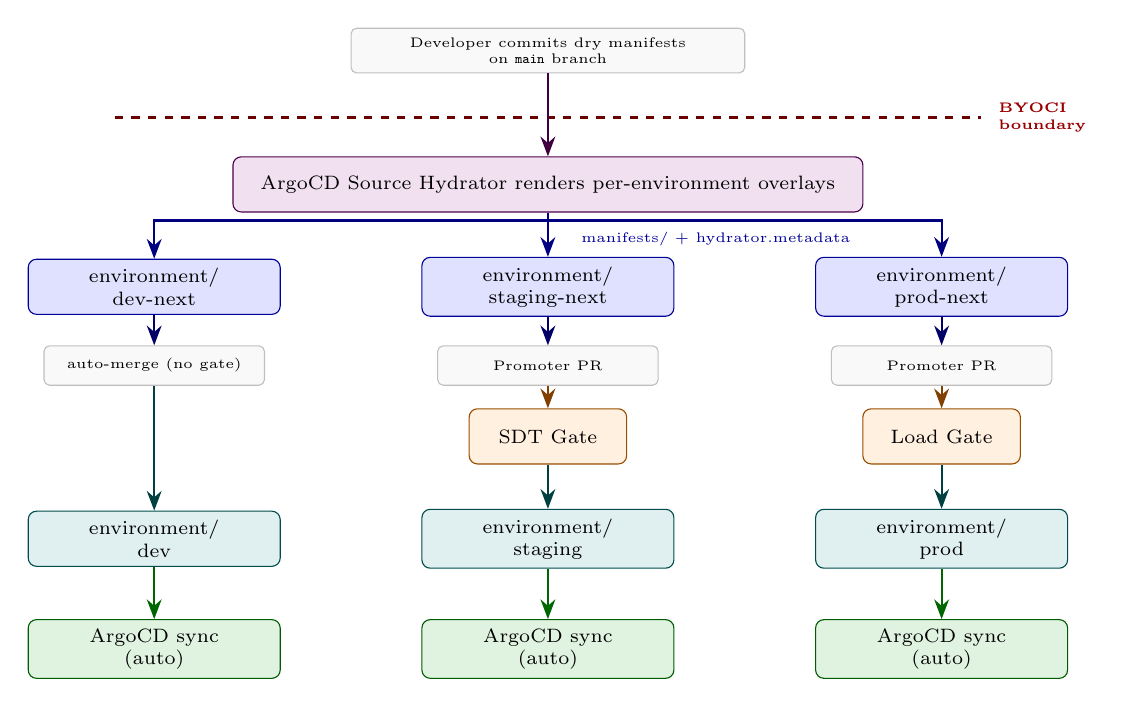
\begin{tikzpicture}[
    >={Stealth[length=2.5mm]},
    branch/.style={
        rectangle,
        rounded corners=3pt,
        draw=#1!60!black,
        fill=#1!12,
        minimum width=3.2cm,
        minimum height=0.7cm,
        font=\scriptsize,
        align=center
    },
    action/.style={
        rectangle,
        rounded corners=2pt,
        draw=gray!50,
        fill=gray!5,
        minimum width=2.8cm,
        minimum height=0.5cm,
        font=\tiny,
        align=center
    },
    boundary/.style={
        dashed,
        thick,
        #1!60!black
    }
]

% Developer commit on main (top)
\node[action, minimum width=5cm] (push) at (5,0) {Developer commits dry manifests\\on \texttt{main} branch};

% BYOCI boundary line and side-anchored label
% The dashed boundary separates the developer's side (above) from the
% XSDLC platform side (below). One single label is anchored at the
% right edge, positioned to the right of the box stack so it does not
% collide with any other element.
\draw[boundary=red!70!black] (-0.5,-0.85) -- (10.5,-0.85);
\node[font=\tiny\bfseries,text=red!60!black,anchor=west,align=left]
  at (10.6,-0.85)
  {BYOCI\\boundary};

% ArgoCD Hydrator step
\node[branch=violet, minimum width=8cm] (hydrator) at (5,-1.7) {ArgoCD Source Hydrator renders per-environment overlays};

\draw[->,thick,violet!50!black] (push.south) -- (hydrator.north);

% env-next branches in gitops repo
\node[branch=blue] (devnext)     at (0,-3.0) {environment/\\dev-next};
\node[branch=blue] (stagingnext) at (5,-3.0) {environment/\\staging-next};
\node[branch=blue] (prodnext)    at (10,-3.0) {environment/\\prod-next};

\draw[->,thick,blue!50!black] (hydrator.south) -- ++(0,-0.1) -| (devnext.north);
\draw[->,thick,blue!50!black] (hydrator.south) -- (stagingnext.north);
\draw[->,thick,blue!50!black] (hydrator.south) -- ++(0,-0.1) -| (prodnext.north);

% Label showing hydrated output — anchored next to the centred
% staging-next arrow so it sits over empty space rather than crossing
% other arrows or boxes.
\node[font=\tiny,text=blue!60!black,anchor=west] at (5.3,-2.4) {manifests/ + hydrator.metadata};

% Promoter PRs
\node[action] (pr1) at (0,-4.0) {auto-merge (no gate)};
\node[action] (pr2) at (5,-4.0) {Promoter PR};
\node[action] (pr3) at (10,-4.0) {Promoter PR};

\draw[->,thick,blue!40!black] (devnext) -- (pr1);
\draw[->,thick,blue!40!black] (stagingnext) -- (pr2);
\draw[->,thick,blue!40!black] (prodnext) -- (pr3);

% Quality gates
\node[branch=orange, minimum width=2cm] (gate1) at (5,-4.9) {SDT Gate};
\node[branch=orange, minimum width=2cm] (gate2) at (10,-4.9) {Load Gate};

\draw[->,thick,orange!50!black] (pr2) -- (gate1);
\draw[->,thick,orange!50!black] (pr3) -- (gate2);

% Active branches
% Round-2 review [264]: row moved from y=-5.8 to y=-6.2. The two-line branch
% nodes previously left <2.5mm between the gate's south border and the branch
% node's north border, so the gate1->staging arrow (head longer than the gap)
% rendered clipped. All arrows are now border-anchored with room to render
% completely, which also restores a correct bounding box.
\node[branch=teal] (dev)     at (0,-6.2) {environment/\\dev};
\node[branch=teal] (staging) at (5,-6.2) {environment/\\staging};
\node[branch=teal] (prod)    at (10,-6.2) {environment/\\prod};

\draw[->,thick,teal!50!black] (pr1.south) -- (dev.north);
\draw[->,thick,teal!50!black] (gate1.south) -- (staging.north);
\draw[->,thick,teal!50!black] (gate2.south) -- (prod.north);

% ArgoCD sync (all auto)
\node[branch=green!60!black] (argodev) at (0,-7.6) {ArgoCD sync\\(auto)};
\node[branch=green!60!black] (argostg) at (5,-7.6) {ArgoCD sync\\(auto)};
\node[branch=green!60!black] (argoprod) at (10,-7.6) {ArgoCD sync\\(auto)};

\draw[->,thick,green!40!black] (dev.south) -- (argodev.north);
\draw[->,thick,green!40!black] (staging.south) -- (argostg.north);
\draw[->,thick,green!40!black] (prod.south) -- (argoprod.north);

\end{tikzpicture}
%
}
\caption{Single-repo branch topology. The developer triggers \texttt{driveby-deploy.yml} to push manifests from \texttt{main} to a single \texttt{-next} branch; the Promoter creates PRs to active branches; quality gates control promotion; ArgoCD syncs from active branches. The BYOCI boundary is annotated: developer CI ends at \texttt{main}, XSDLC delivery begins at the deploy step.}
\label{fig:single-repo-branch-flow}
\end{figure}

The branch graph flows from \texttt{main} through the deploy workflow to a single \texttt{environment/<name>-next} branch per trigger. The Promoter creates promotion PRs from each \texttt{-next} branch to its active \texttt{environment/<name>} branch. Quality gates (when defined) evaluate before the PR is merged. ArgoCD watches each active branch and syncs the corresponding namespace.

% ============================================================================
\section{Multi-Environment Promotion}
\label{sec:multi-env-promotion}
% ============================================================================

The GitOps Promoter~\cite{gitops-promoter} automates environment promotion by watching for commit status signals and managing promotion pull requests. Figure~\ref{fig:multi-env-promotion} shows the three-environment model.

\begin{figure}[htbp]
\centering
\resizebox{\textwidth}{!}{%
% Multi-Environment Promotion — Chapter 6
% Shows: dev → staging → prod with quality gates between them
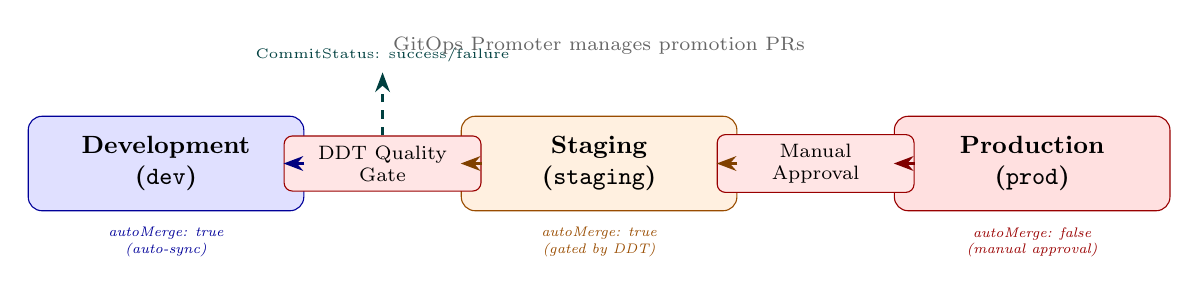
\begin{tikzpicture}[
    >={Stealth[length=2.5mm]},
    node distance=1.5cm,
    env/.style={
        rectangle,
        rounded corners=5pt,
        draw=#1!60!black,
        fill=#1!12,
        minimum width=3.5cm,
        minimum height=1.2cm,
        font=\small\bfseries,
        align=center
    },
    gate/.style={
        rectangle,
        rounded corners=3pt,
        draw=red!60!black,
        fill=red!10,
        minimum width=2.5cm,
        minimum height=0.7cm,
        font=\scriptsize,
        align=center
    },
    policy/.style={
        font=\tiny\itshape,
        text=#1!60!black,
        align=center
    }
]

% Environments
\node[env=blue] (dev) at (0,0) {Development\\(\texttt{dev})};
\node[env=orange] (staging) at (5.5,0) {Staging\\(\texttt{staging})};
\node[env=red] (prod) at (11,0) {Production\\(\texttt{prod})};

% Quality gates
\node[gate] (gate1) at (2.75,0) {DDT Quality\\Gate};
\node[gate] (gate2) at (8.25,0) {Manual\\Approval};

% Arrows
\draw[->,thick,blue!50!black] (dev) -- (gate1);
\draw[->,thick,orange!50!black] (gate1) -- (staging);
\draw[->,thick,orange!50!black] (staging) -- (gate2);
\draw[->,thick,red!50!black] (gate2) -- (prod);

% Policies
\node[policy=blue] at (0,-1.0) {autoMerge: true\\(auto-sync)};
\node[policy=orange] at (5.5,-1.0) {autoMerge: true\\(gated by DDT)};
\node[policy=red] at (11,-1.0) {autoMerge: false\\(manual approval)};

% Commit status flow
\draw[->,dashed,teal!50!black,thick] (gate1.north) -- ++(0,0.8) node[above,font=\tiny,teal!50!black] {CommitStatus: success/failure};

% Promoter label
\node[font=\scriptsize,text=black!60] at (5.5,1.5) {GitOps Promoter manages promotion PRs};

\end{tikzpicture}
%
}
\caption{Multi-environment promotion model. Development auto-syncs; staging promotion is gated by DDT validation (commit status); production requires manual approval.}
\label{fig:multi-env-promotion}
\end{figure}

% ----------------------------------------------------------------------------
\subsection{PromotionStrategy}
\label{subsec:promotion-strategy}
% ----------------------------------------------------------------------------

The PromotionStrategy custom resource defines the environment chain and the commit status keys that gate each transition. For the reference deployment, the strategy specifies three environments:

\begin{enumerate}
    \item \textbf{Development} (\texttt{dev} branch, \texttt{autoMerge: true}). Changes from the deploy workflow are automatically merged by the Promoter. No quality gate---development is the environment where new code lands first.
    \item \textbf{Staging} (\texttt{staging} branch, \texttt{autoMerge: true}). Promotion from development to staging is gated by the \texttt{staging-gate} commit status (the default key derived from the environment name). The Promoter creates a promotion PR, waits for the commit status to report success, and merges automatically. If the commit status reports failure, the PR remains open and promotion is blocked.
    \item \textbf{Production} (\texttt{prod} branch, \texttt{autoMerge: false}). Promotion from staging to production requires manual approval. A human reviewer must merge the promotion PR, providing a final checkpoint before production deployment.
\end{enumerate}

This two-tier model balances automation with safety. Development and staging promotions are fully automated (with DDT gating the staging transition); production promotion retains human oversight. Teams can adjust the \texttt{autoMerge} setting per environment to match their risk tolerance.

% ----------------------------------------------------------------------------
\subsection{CommitStatus as Quality Signal}
\label{subsec:commit-status-signal}
% ----------------------------------------------------------------------------

The integration between DriveBy and the GitOps Promoter is mediated by two commit status mechanisms:

\textbf{GitHub commit status.} The workflow's set-pending and report-success steps post commit status updates to the PR's head SHA via the GitHub API. The context key (e.g., \texttt{staging-gate}) is watched by the PromotionStrategy as the gate signal. This mechanism works for any GitHub-based workflow and does not require the GitOps Promoter.

\textbf{CommitStatus CRD.} When the GitOps Promoter is enabled, the workflow additionally creates a CommitStatus custom resource in the \texttt{driveby} namespace. The CommitStatus transitions through three phases: \texttt{pending} (set at workflow start), \texttt{success} (set after validation passes), or \texttt{failure} (set by the exit handler). The Promoter controller watches this resource and uses its phase to determine whether to merge the promotion PR. This CRD-based mechanism provides a Kubernetes-native alternative to the GitHub API and enables the Promoter to function even in environments where direct GitHub API access is restricted.

% ----------------------------------------------------------------------------
\subsection{ChangeTransferPolicy}
\label{subsec:change-transfer-policy}
% ----------------------------------------------------------------------------

The ChangeTransferPolicy defines how changes flow between environments at the Git level. For each environment, the policy maps a \textit{proposed} branch (e.g., \texttt{staging-next}) to an \textit{active} branch (e.g., \texttt{staging}). The Promoter creates pull requests from the proposed branch to the active branch and merges them when commit status gates pass. This branch-based model integrates naturally with Git-based review workflows: promotion PRs appear in the repository's PR list, carry commit status checks, and leave an auditable merge history.

% ----------------------------------------------------------------------------
\subsection{Promoter Reconciliation Loop}
\label{subsec:promoter-reconciliation}
% ----------------------------------------------------------------------------

The GitOps Promoter is itself a Kubernetes controller that implements the observe-diff-act pattern (Section~\ref{subsec:reconciliation-loop}) at the Git level rather than the cluster level.

\textbf{Observe.} The PromotionStrategy controller watches two resource types: GitRepository (which tracks the application repository) and CommitStatus (which reports quality gate results). It periodically polls the Git repository to detect changes on proposed branches and reads CommitStatus resources to determine gate outcomes.

\textbf{Diff.} For each environment in the promotion chain, the controller compares the proposed branch (\texttt{environment/<name>-next}) against the active branch (\texttt{environment/<name>}). If the branches differ, a promotion is pending. It then checks whether all required CommitStatuses report \texttt{success}. If any CommitStatus reports \texttt{failure} or \texttt{pending}, the promotion is blocked.

\textbf{Act.} When the proposed and active branches differ, the controller creates a promotion PR. When all commit status gates pass and \texttt{autoMerge} is \texttt{true}, the controller merges the PR automatically. When \texttt{autoMerge} is \texttt{false}, the PR remains open for human review.

The ChangeTransferPolicy is itself a second reconciliation layer: it is auto-created by the PromotionStrategy controller when the PromotionStrategy is applied. The PromotionStrategy reconciles the \textit{promotion logic} (which environments exist, what gates are required); the ChangeTransferPolicy reconciles the \textit{branch mechanics} (which branches map to which environments, when to create PRs). This two-layer design separates strategic configuration (the promotion chain) from tactical execution (the branch operations).

% ============================================================================
\section{Human-in-the-Loop Patterns}
\label{sec:human-in-the-loop}
% ============================================================================

The quality gate system is not fully autonomous. It automates objective assessments---DDT validation, health checks, load testing---while preserving human judgment for subjective assessments. This section maps the automation spectrum and identifies the decision points where human intervention is required or optional.

% ----------------------------------------------------------------------------
\subsection{The Automation Spectrum}
\label{subsec:automation-spectrum}
% ----------------------------------------------------------------------------

The system supports four points on the automation spectrum, controlled by two boolean parameters: \texttt{autoMerge} (on the PromotionStrategy, controlling whether the Promoter automatically merges promotion PRs) and \texttt{automated.selfHeal} (on the ArgoCD Application, controlling whether ArgoCD automatically syncs and self-heals).

\begin{enumerate}
    \item \textbf{Fully automated} (development): \texttt{autoMerge: true}, automated sync. After the developer triggers a deploy, changes flow from the \texttt{-next} branch, are auto-merged by the Promoter, and auto-synced by ArgoCD. No further human intervention after the initial trigger.
    \item \textbf{Automated with quality gate} (staging): \texttt{autoMerge: true}, automated sync, with a commit status gate. The Promoter waits for DDT validation to report success before merging. If validation fails, the PR remains open until the developer fixes the issue and re-pushes. Once the gate passes, promotion and sync are automatic.
    \item \textbf{Gated with human approval} (production): \texttt{autoMerge: false}, manual sync. The Promoter creates the PR and DDT validates the source environment, but a human must explicitly merge the promotion PR. Even after merge, ArgoCD requires manual sync (since automated sync is disabled). Two human checkpoints bookend the quality gate.
    \item \textbf{Fully manual}: no quality gate, manual merge, manual sync. This mode is possible but unused in the reference deployment---it offers no advantage over the gated model.
\end{enumerate}

% ----------------------------------------------------------------------------
\subsection{Decision Points}
\label{subsec:decision-points}
% ----------------------------------------------------------------------------

Figure~\ref{fig:human-in-the-loop} maps the decision points across the staging and production lanes.

\begin{figure}[htbp]
\centering
\resizebox{\textwidth}{!}{%
% Human-in-the-Loop — Chapter 6, Section 6.5.2
% Pipeline with green (automated) and amber (human) steps for staging vs prod
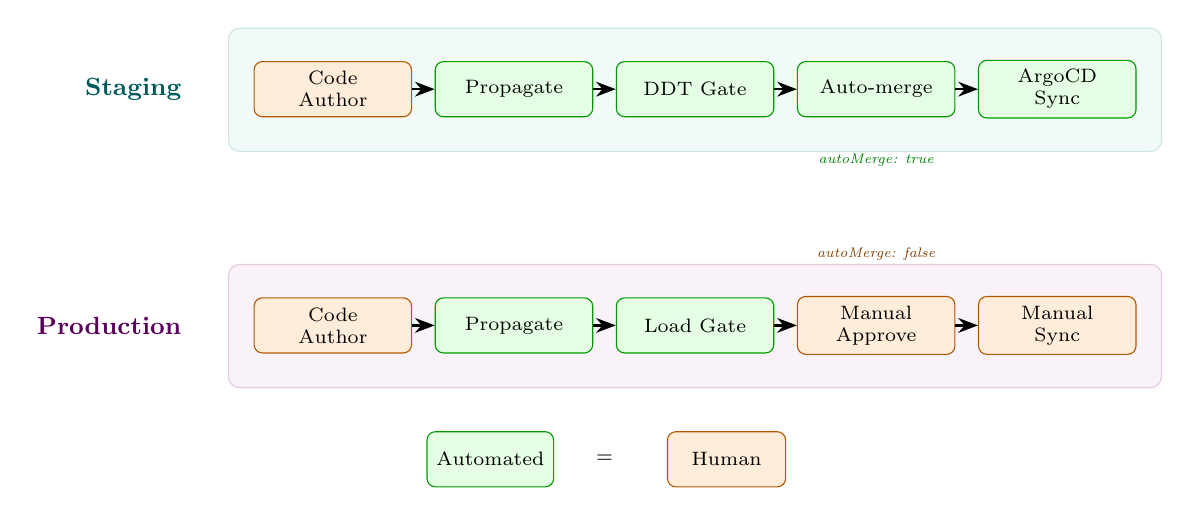
\begin{tikzpicture}[
    >={Stealth[length=2.5mm]},
    auto step/.style={
        rectangle,
        rounded corners=3pt,
        draw=green!60!black,
        fill=green!10,
        minimum width=2cm,
        minimum height=0.7cm,
        font=\scriptsize,
        align=center
    },
    human step/.style={
        rectangle,
        rounded corners=3pt,
        draw=orange!70!black,
        fill=orange!15,
        minimum width=2cm,
        minimum height=0.7cm,
        font=\scriptsize,
        align=center
    },
    lane label/.style={
        font=\small\bfseries,
        text=#1!70!black,
        anchor=east
    }
]

% Lane labels
\node[lane label=teal] at (-0.3,1.5) {Staging};
\node[lane label=violet] at (-0.3,-1.5) {Production};

% Staging lane (mostly automated)
\node[human step] (s1) at (1.5,1.5) {Code\\Author};
\node[auto step]  (s2) at (3.8,1.5) {Propagate};
\node[auto step]  (s3) at (6.1,1.5) {DDT Gate};
\node[auto step]  (s4) at (8.4,1.5) {Auto-merge};
\node[auto step]  (s5) at (10.7,1.5) {ArgoCD\\Sync};

\draw[->,thick] (s1) -- (s2);
\draw[->,thick] (s2) -- (s3);
\draw[->,thick] (s3) -- (s4);
\draw[->,thick] (s4) -- (s5);

% Production lane (human checkpoints)
\node[human step] (p1) at (1.5,-1.5) {Code\\Author};
\node[auto step]  (p2) at (3.8,-1.5) {Propagate};
\node[auto step]  (p3) at (6.1,-1.5) {Load Gate};
\node[human step] (p4) at (8.4,-1.5) {Manual\\Approve};
\node[human step] (p5) at (10.7,-1.5) {Manual\\Sync};

\draw[->,thick] (p1) -- (p2);
\draw[->,thick] (p2) -- (p3);
\draw[->,thick] (p3) -- (p4);
\draw[->,thick] (p4) -- (p5);

% Lane backgrounds
\begin{scope}[on background layer]
    \node[rectangle, rounded corners=4pt, fill=teal!5, draw=teal!20,
          fit={($(s1.north west)+(-0.2,0.3)$) ($(s5.south east)+(0.2,-0.3)$)}] {};
    \node[rectangle, rounded corners=4pt, fill=violet!5, draw=violet!20,
          fit={($(p1.north west)+(-0.2,0.3)$) ($(p5.south east)+(0.2,-0.3)$)}] {};
\end{scope}

% Legend
\node[auto step, minimum width=1.5cm] (leg1) at (3.5,-3.2) {Automated};
\node[human step, minimum width=1.5cm] (leg2) at (6.5,-3.2) {Human};
\node[font=\scriptsize] at (4.95,-3.2) {=};

% Annotation arrows for key decisions
\node[font=\tiny\itshape,text=green!50!black] at (8.4,0.6) {autoMerge: true};
\node[font=\tiny\itshape,text=orange!50!black] at (8.4,-0.6) {autoMerge: false};

\end{tikzpicture}
%
}
\caption{Human-in-the-loop patterns. Staging automates everything except code authorship; production adds human approval at the promotion PR merge and ArgoCD sync points. Green steps are automated; amber steps require human judgment.}
\label{fig:human-in-the-loop}
\end{figure}

All human intervention points in the system are:

\begin{enumerate}
    \item \textbf{Code authorship}: the developer writes the code and updates manifests. This is inherently human (or human-supervised, in the case of AI-assisted development).
    \item \textbf{PR review} (\texttt{autoMerge: false}): a human reviews the promotion PR and decides whether to merge. This checkpoint applies to production promotions, where the decision involves business timing, release coordination, and risk assessment---subjective factors that DDT does not measure.
    \item \textbf{ArgoCD sync} (manual sync): a human triggers synchronization in the ArgoCD UI. This checkpoint ensures that production deployments are initiated deliberately, not as an automatic consequence of a merge.
    \item \textbf{Failure diagnosis}: when a quality gate fails, a human (or autonomous agent) must diagnose the failure, fix the issue, and re-push. The DDT validation report provides per-principle diagnostics to guide this process.
\end{enumerate}

% ----------------------------------------------------------------------------
\subsection{Automation with Human Override}
\label{subsec:automation-override}
% ----------------------------------------------------------------------------

The design philosophy is: \textit{automate objective assessments, preserve human judgment for subjective assessments}. DDT validation, health checks, and load testing produce binary signals (pass/fail) based on measurable criteria. These are objective and automatable. Production readiness, business timing, and release coordination involve context that no automated system can capture. These are subjective and require human judgment.

The \texttt{autoMerge: false} setting is a deliberate architectural choice, not a limitation. It reflects the principle that the final decision to deploy to production should be an affirmative human act, even when all automated checks have passed. The quality gate provides confidence; the human provides authorization.

% ============================================================================
\section{Quality Gate as Control Loop}
\label{sec:control-loop}
% ============================================================================

This section synthesizes the architectural components described in Chapters~\ref{ch:architecture},~\ref{ch:kubernetes}, and the preceding sections of this chapter into a single control-theoretic framework. The quality gate system implements a \textit{closed-loop negative feedback} controller~\cite{astrom-feedback} that maintains API quality across the delivery pipeline.

% ----------------------------------------------------------------------------
\subsection{Control Theory Mapping}
\label{subsec:control-mapping}
% ----------------------------------------------------------------------------

The mapping from control theory to the DriveBy quality gate system is direct:

\begin{description}
    \item[Desired State (Setpoint):] The OpenAPI specification declares the desired API contract---the schemas, operations, error responses, security definitions, and documentation that the API should provide. This is the reference input against which the system measures deviation.

    \item[Plant:] The API deployment in the source environment (e.g., \texttt{perfect-api-dev}) is the controlled process. Its behavior---response schemas, error codes, latency characteristics---is the output being regulated.

    \item[Sensor:] The DriveBy CLI is the measurement instrument. It observes the plant's output by fetching the specification, validating it against the DDT principles, and producing a structured report. The sensor converts the plant's complex, multidimensional behavior into a scalar quality signal (pass/fail per principle, aggregate score).

    \item[Controller:] The Argo Workflow DAG is the decision-making component. It orchestrates the sensor (DriveBy validation steps), evaluates the results, and produces a control signal. The controller implements a simple threshold policy: if all checks pass, emit ``success''; if any check fails, emit ``failure''. The exit handler guarantees that the controller always produces a signal---no workflow terminates without an explicit quality verdict.

    \item[Actuator:] The CommitStatus CRD and the GitOps Promoter together form the actuator---the component that translates the control signal into physical action. A ``success'' signal causes the Promoter to merge the promotion PR, advancing the deployment. A ``failure'' signal causes the Promoter to hold the PR open, blocking advancement.

    \item[Feedback Loop:] The Promoter closes the loop. When promotion is blocked (failure signal), the developer must diagnose the issue, fix the code or specification, and re-trigger the deploy workflow. The new manifests update the \texttt{-next} branch, the Promoter updates the PR, and the quality gate re-evaluates. The system iterates until the plant's behavior converges with the desired state.
\end{description}

Figure~\ref{fig:quality-control-loop} illustrates this mapping.

\begin{figure}[htbp]
\centering
\resizebox{\textwidth}{!}{%
% Quality Gate as Control Loop — Chapter 6, Section 6.6
% Control theory block diagram: Setpoint (promotion policy) → Controller → Actuator → Plant (delivery system) → Sensor → feedback
% Mapping kept in lockstep with Table 6.1 (tab:control-mapping):
%   Setpoint = promotion-policy predicate (OpenAPI spec + XSDLC manifest)
%   Plant    = delivery system (pipeline + promotion workflow)
%   Actuator = CommitStatus + Promoter (merges/blocks promotion PR — acts ON the delivery system)
%   Sensor   = DriveBy CLI; measurement = validation verdict
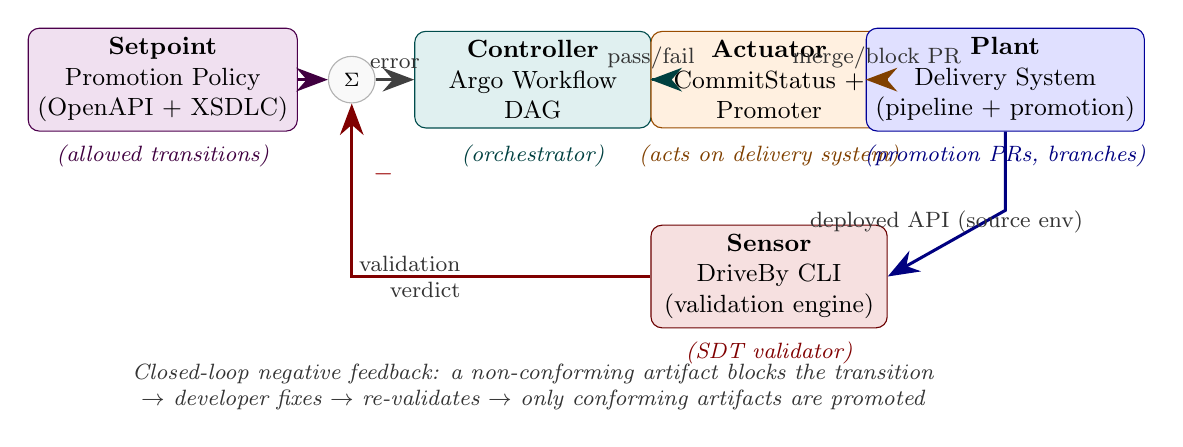
\begin{tikzpicture}[
    >={Stealth[length=4mm,width=3mm]},
    block/.style={
        rectangle,
        rounded corners=4pt,
        draw=#1!60!black,
        fill=#1!12,
        minimum width=3cm,
        minimum height=1cm,
        font=\small,
        align=center
    },
    signal/.style={
        font=\footnotesize,
        text=gray!40!black
    },
    sum/.style={
        circle,
        draw=gray!60,
        fill=gray!5,
        minimum size=0.5cm,
        font=\scriptsize
    },
    flow/.style={->,line width=1.1pt}
]

% Setpoint: promotion-policy predicate
\node[block=violet] (setpoint) at (0,0) {\textbf{Setpoint}\\Promotion Policy\\(OpenAPI $+$ XSDLC)};

% Sum point
\node[sum] (sum) at (2.4,0) {$\Sigma$};

% Controller
\node[block=teal] (controller) at (4.7,0) {\textbf{Controller}\\Argo Workflow\\DAG};

% Actuator
\node[block=orange] (actuator) at (7.7,0) {\textbf{Actuator}\\CommitStatus +\\Promoter};

% Plant: the delivery system
\node[block=blue] (plant) at (10.7,0) {\textbf{Plant}\\Delivery System\\(pipeline $+$ promotion)};

% Sensor
\node[block=red!70!black] (sensor) at (7.7,-2.5) {\textbf{Sensor}\\DriveBy CLI\\(validation engine)};

% Forward path
\draw[flow,violet!50!black] (setpoint) -- (sum);
\draw[flow,gray!50!black] (sum) -- node[above,signal] {error} (controller);
\draw[flow,teal!50!black] (controller) -- node[above,signal] {pass/fail} (actuator);
\draw[flow,orange!50!black] (actuator) -- node[above,signal] {merge/block PR} (plant);

% Feedback path: the plant's deployed API (source env) is measured by the sensor
\draw[flow,blue!50!black] (plant.south) -- ++(0,-1) -- node[above,signal] {deployed API (source env)} (sensor.east);
\draw[flow,red!50!black] (sensor.west) -| node[left,signal,pos=0.3,align=right] {validation\\verdict} (sum.south);

% Negative feedback annotation
\node[font=\small\bfseries,text=red!60!black] at (2.8,-1.2) {$-$};

% Labels for control theory mapping
\node[font=\footnotesize\itshape,text=violet!50!black,anchor=north] at (0,-0.7) {(allowed transitions)};
\node[font=\footnotesize\itshape,text=teal!50!black,anchor=north] at (4.7,-0.7) {(orchestrator)};
\node[font=\footnotesize\itshape,text=orange!50!black,anchor=north] at (7.7,-0.7) {(acts on delivery system)};
\node[font=\footnotesize\itshape,text=blue!50!black,anchor=north] at (10.7,-0.7) {(promotion PRs, branches)};
\node[font=\footnotesize\itshape,text=red!50!black,anchor=north] at (7.7,-3.2) {(SDT validator)};

% Convergence annotation
\node[font=\footnotesize\itshape,text=gray!40!black,align=center] at (4.7,-3.9) {Closed-loop negative feedback: a non-conforming artifact blocks the transition\\$\rightarrow$ developer fixes $\rightarrow$ re-validates $\rightarrow$ only conforming artifacts are promoted};

\end{tikzpicture}
%
}
\caption{Quality gate as control loop. The OpenAPI specification is the setpoint; the DriveBy CLI is the sensor; the Argo Workflow is the controller; the CommitStatus and Promoter form the actuator. Negative feedback blocks promotion on validation failure, driving convergence.}
\label{fig:quality-control-loop}
\end{figure}

% ----------------------------------------------------------------------------
\subsection{Negative Feedback and Convergence}
\label{subsec:negative-feedback}
% ----------------------------------------------------------------------------

The feedback is \textit{negative}: validation failure produces a signal that opposes the direction of change (blocking promotion rather than advancing it). This is the defining characteristic of a regulating control loop~\cite{astrom-feedback}. Without negative feedback, a failing API would be promoted to staging and then to production, with quality problems detected only after deployment---the shift-right antipattern that DDT explicitly prevents.

The convergence dynamics depend on the developer response. Each quality gate evaluation is a discrete sampling of the plant's state. The developer's fix attempt modifies the plant. The next evaluation samples the modified state. If the fix addresses the failing principle, the quality signal transitions from ``failure'' to ``success'' and the loop converges. If the fix is incomplete, the signal remains ``failure'' and the loop iterates.

The level-triggered nature of the Kubernetes controller pattern (Section~\ref{subsec:reconciliation-loop}) ensures that the control loop is robust to transient failures. If a workflow fails due to infrastructure issues (pod eviction, network timeout) rather than validation failure, the exit handler posts a ``failure'' status. The developer re-pushes (or the Promoter detects the branch change), and the workflow re-executes. The system does not require manual re-triggering because the Promoter continuously reconciles the branch state.

% ----------------------------------------------------------------------------
\subsection{Connecting Theory to Implementation}
\label{subsec:theory-implementation}
% ----------------------------------------------------------------------------

This control-theoretic framing connects the abstract ontological state reconciliation pattern introduced in Section~\ref{subsec:ontological-reconciliation} of Chapter~\ref{ch:related-work} to the concrete implementation described in this thesis.

In Section~\ref{subsec:ontological-reconciliation}, we defined ontological state reconciliation as requiring three components: an ontological artifact (the specification), a reconciliation agent (the validator), and a correction mechanism (the quality gate). The control loop formalization adds precision: the specification is the setpoint, the validator is the sensor, and the quality gate is the controller-actuator pair that closes the feedback loop.

The three DDT axioms map directly to control-theoretic requirements. The \textit{Axiom of Completeness} requires that the setpoint (specification) is expressive enough to fully characterize the desired behavior---an incomplete setpoint produces an under-determined control loop that cannot distinguish conforming from non-conforming behavior. The \textit{Axiom of Determinism} requires that the sensor (validator) produces consistent measurements---a non-deterministic sensor would cause the control loop to oscillate between pass and fail for identical plant states. The \textit{Axiom of Observability} requires that the sensor's output is structured and actionable---an unobservable control loop cannot inform corrective action, and the feedback degenerates into a binary gate with no diagnostic value.

The quality gate system thus instantiates a well-defined control loop in which every component---setpoint, sensor, controller, actuator, and feedback path---has a concrete implementation in the DriveBy architecture. This is not a metaphorical mapping; it is a structural correspondence that explains why the system converges, why it is robust to transient failures, and why the axiomatic foundation is necessary rather than merely desirable.

% ============================================================================
\section{CI/CD of DriveBy Itself}
\label{sec:cicd-driveby}
% ============================================================================

DriveBy's own development is governed by three GitHub Actions~\cite{github-actions} workflows that implement continuous integration, continuous delivery, and release automation. These pipelines demonstrate that the project practices what it preaches: automated quality gates at every stage of the delivery lifecycle.

% ----------------------------------------------------------------------------
\subsection{Continuous Integration}
\label{subsec:ci-pipeline}
% ----------------------------------------------------------------------------

The \texttt{ci.yml} workflow triggers on every push to \texttt{main} and every pull request. It runs a single \texttt{build-and-test} job on Ubuntu with Go~1.21 that executes four steps:

\begin{enumerate}
    \item \textbf{Build}: Compiles the DriveBy binary with version and commit SHA injected via \texttt{ldflags}.
    \item \textbf{Static analysis}: Runs \texttt{go vet} to detect common Go errors.
    \item \textbf{Test}: Executes the test suite from \texttt{driveby-cli/test/} with coverage profiling (\texttt{-coverprofile=coverage.out}).
    \item \textbf{Documentation check}: Runs \texttt{tools/check-docs.sh} to verify that all documented components exist and all source files have corresponding documentation entries.
\end{enumerate}

The documentation check is a meta-validation step: it ensures that the CLAUDE.md files and documentation artifacts remain synchronized with the codebase. This check embodies a DDT-adjacent principle---documentation completeness should be verified automatically, not assumed.

On pull requests, the workflow uploads the coverage artifact for review. On pushes to \texttt{main}, a subsequent \texttt{docker} job builds the container image (without pushing) to verify the Docker build remains functional.

% ----------------------------------------------------------------------------
\subsection{Docker Image Publishing}
\label{subsec:docker-publish}
% ----------------------------------------------------------------------------

The \texttt{docker-publish.yml} workflow publishes container images to the GitHub Container Registry (GHCR) on pushes to \texttt{main} when files in \texttt{driveby-cli/} change. It uses Docker Buildx~\cite{docker-buildx} for multi-platform builds, injecting three build arguments:

\begin{itemize}
    \item \texttt{VERSION}: The current Git tag or \texttt{dev} for unreleased commits.
    \item \texttt{COMMIT}: The short Git SHA.
    \item \texttt{BUILD\_DATE}: The ISO-8601 build timestamp.
\end{itemize}

Images are tagged with \texttt{latest} and the short commit SHA. Layer caching via GitHub Actions Cache reduces build times for incremental changes. The resulting image at \texttt{ghcr.io/meter-peter/driveby} is the same image used by the Argo Workflows validation pipeline.

% ----------------------------------------------------------------------------
\subsection{Release Pipeline}
\label{subsec:release-pipeline}
% ----------------------------------------------------------------------------

The \texttt{release.yml} workflow triggers on semantic version tag pushes (\texttt{v*}) and orchestrates the full release process. Figure~\ref{fig:release-pipeline} shows the pipeline structure.

\begin{figure}[htbp]
\centering
\resizebox{\textwidth}{!}{%
% Release Pipeline — Chapter 6
% Shows: Tag push → test gate → goreleaser + docker + helm (parallel fan-out)
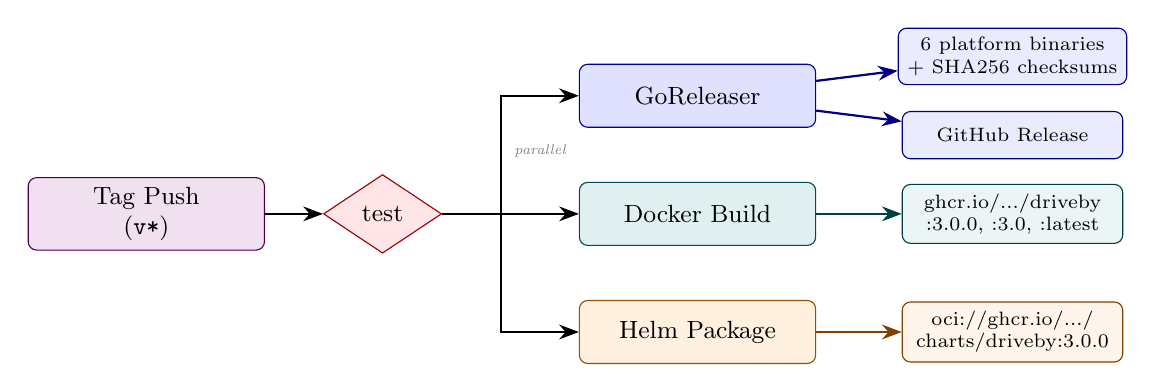
\begin{tikzpicture}[
    >={Stealth[length=2.5mm]},
    node distance=0.9cm,
    stage/.style={
        rectangle,
        rounded corners=3pt,
        draw=#1!60!black,
        fill=#1!12,
        minimum width=3cm,
        minimum height=0.8cm,
        font=\small,
        align=center
    },
    gate/.style={
        diamond,
        draw=red!60!black,
        fill=red!10,
        minimum width=1.5cm,
        minimum height=1cm,
        font=\small,
        align=center,
        inner sep=1pt
    },
    artifact/.style={
        rectangle,
        rounded corners=3pt,
        draw=#1!50!black,
        fill=#1!8,
        minimum width=2.8cm,
        minimum height=0.6cm,
        font=\scriptsize,
        align=center
    }
]

% Trigger
\node[stage=violet] (tag) at (0,0) {Tag Push\\(\texttt{v*})};

% Test gate
\node[gate] (test) at (3,0) {test};
\draw[->,thick] (tag) -- (test);

% Fan-out (three parallel jobs)
\node[stage=blue] (goreleaser) at (7,1.5) {GoReleaser};
\node[stage=teal] (docker) at (7,0) {Docker Build};
\node[stage=orange] (helm) at (7,-1.5) {Helm Package};

\draw[->,thick] (test) -- ++(1.5,0) |- (goreleaser);
\draw[->,thick] (test) -- (docker);
\draw[->,thick] (test) -- ++(1.5,0) |- (helm);

% Fan-out label
\node[font=\tiny\itshape,text=black!50] at (5,0.8) {parallel};

% Artifacts
\node[artifact=blue] (bins) at (11,2.0) {6 platform binaries\\+ SHA256 checksums};
\node[artifact=blue] (release) at (11,1.0) {GitHub Release};
\node[artifact=teal] (image) at (11,0) {ghcr.io/.../driveby\\:3.0.0, :3.0, :latest};
\node[artifact=orange] (chart) at (11,-1.5) {oci://ghcr.io/.../\\charts/driveby:3.0.0};

\draw[->,thick,blue!50!black] (goreleaser) -- (bins);
\draw[->,thick,blue!50!black] (goreleaser) -- (release);
\draw[->,thick,teal!50!black] (docker) -- (image);
\draw[->,thick,orange!50!black] (helm) -- (chart);

\end{tikzpicture}
%
}
\caption{Release pipeline triggered by a version tag push. After the test gate passes, three parallel jobs produce platform binaries, Docker images, and a Helm chart.}
\label{fig:release-pipeline}
\end{figure}

The pipeline runs four jobs:

\textbf{Test gate.} Re-runs \texttt{go vet} and the test suite. All subsequent jobs depend on this gate---no artifacts are produced if tests fail.

\textbf{GoReleaser.} Uses GoReleaser~\cite{goreleaser}~v2 to produce cross-compiled binaries for six platforms: Linux, macOS, and Windows on both amd64 and arm64 architectures. GoReleaser generates SHA256 checksums for each binary and creates a GitHub Release with the binaries, checksums, and an auto-generated changelog attached. The release changelog summarizes commits since the previous tag.

\textbf{Docker.} Builds and pushes the container image with three semver-derived tags: the full version (\texttt{0.4.0}), the major.minor (\texttt{0.4}), and \texttt{latest}. This tagging strategy enables consumers to pin to a specific patch version, track a minor version, or always use the latest release.

\textbf{Helm.} Packages the Helm chart from \texttt{kubernetes/helm/driveby/} and pushes it to the OCI registry at \texttt{oci://ghcr.io/meter-peter/charts/driveby}. The chart version matches the release tag, ensuring that the chart, container image, and CLI binary are version-aligned.

The three artifact-producing jobs run in parallel after the test gate, minimizing release time. A typical release completes in under five minutes from tag push to all artifacts published.

% ============================================================================
\section{Operational Deployment}
\label{sec:operational-deployment}
% ============================================================================

The quality gate system is deployed on \texttt{private.novelcore.org}, a Kubernetes cluster managed by Kubecore with ArgoCD~\cite{argocd}, Crossplane~\cite{crossplane}, Argo Events~\cite{argo-events}, Argo Workflows~\cite{argo-workflows}, Traefik, and cert-manager pre-installed.

% ----------------------------------------------------------------------------
\subsection{Prerequisites}
\label{subsec:prerequisites}
% ----------------------------------------------------------------------------

The deployment assumes six cluster components:

\begin{enumerate}
    \item \textbf{Crossplane} (v1.14+) with the \texttt{provider-kubernetes} provider for managing in-cluster resources.
    \item \textbf{ArgoCD} (v2.8+) for GitOps-based application deployment across dev, staging, and prod namespaces.
    \item \textbf{Argo Workflows} (v3.5+) for container-native workflow execution.
    \item \textbf{Argo Events} (v1.9+) for event-driven workflow triggering.
    \item \textbf{Traefik} (v2.10+) as the Ingress controller for routing webhook traffic.
    \item \textbf{cert-manager} (v1.13+) for automated TLS certificate provisioning.
\end{enumerate}

These components are managed independently of the DriveBy installation and are assumed to be healthy. The DriveBy Helm chart creates resources that reference these components (Ingress resources reference the Traefik ingress class, certificate annotations reference the cert-manager issuer) but does not install them.

% ----------------------------------------------------------------------------
\subsection{Verification}
\label{subsec:verification}
% ----------------------------------------------------------------------------

After deployment, the operator verifies the system through four checks:

\begin{enumerate}
    \item \textbf{Crossplane readiness}: \texttt{kubectl get composite} confirms that XSDLC resources report \texttt{READY=True}.
    \item \textbf{Argo Events health}: \texttt{kubectl get eventbus,eventsource,sensor -n driveby} confirms all three resources are in a ready state.
    \item \textbf{Webhook connectivity}: A test webhook payload sent to the Ingress endpoint returns a 200 response.
    \item \textbf{End-to-end validation}: Opening a test PR on the monitored repository triggers a workflow run. The operator watches \texttt{kubectl get workflows -n driveby} for workflow completion and verifies that commit status and PR comments appear on the test PR.
\end{enumerate}

% ============================================================================
\section{Summary}
\label{sec:pipeline-summary}
% ============================================================================

This chapter described the operational GitOps pipeline that connects DriveBy's validation capabilities to the software delivery lifecycle.

The promotion-driven quality gate (Section~\ref{sec:promotion-driven-gate}) validates the source environment before allowing promotion, implementing the shift-left principle at the deployment boundary. The event-driven pipeline (Section~\ref{sec:event-pipeline-detail}) transforms GitHub webhooks into structured validation workflows with sub-90-second latency. The single-repo architecture (Section~\ref{sec:single-repo}) eliminates config-repo duplication and establishes the BYOCI principle: XSDLC owns delivery (promotion and quality gates) while developers retain full control over their CI pipeline.

The multi-environment promotion model (Section~\ref{sec:multi-env-promotion}) automates the dev $\rightarrow$ staging transition through DDT-gated commit status signals while retaining manual approval for production. The Promoter itself is a reconciliation controller (Section~\ref{subsec:promoter-reconciliation}), implementing observe-diff-act at the Git level. Human-in-the-loop patterns (Section~\ref{sec:human-in-the-loop}) define a clear automation spectrum: objective assessments (validation, load testing) are automated; subjective assessments (production readiness, business timing) are preserved for human judgment.

The quality gate as control loop (Section~\ref{sec:control-loop}) synthesizes the entire system into a control-theoretic framework, mapping the OpenAPI specification to a setpoint, the DriveBy CLI to a sensor, the Argo Workflow to a controller, and the Promoter to an actuator. This closed-loop negative feedback system ensures convergence: validation failure blocks promotion, driving developers to fix issues until the API conforms to its specification. The three DDT axioms---Completeness, Determinism, and Observability---are shown to be necessary conditions for the control loop to function correctly, connecting the theoretical foundations of Chapter~\ref{ch:related-work} (Section~\ref{subsec:ontological-reconciliation}) to the concrete implementation.

The CI/CD pipelines for DriveBy itself (Section~\ref{sec:cicd-driveby}) demonstrate end-to-end release automation: from test gate through parallel artifact production (binaries, images, Helm chart) to registry publication. Together, these sections show that DDT validation integrates naturally into modern GitOps workflows---not as an afterthought bolted onto an existing pipeline, but as a first-class quality gate in a declarative, event-driven, control-theoretic delivery system.

Chapter~\ref{ch:evaluation} evaluates this system empirically, measuring DDT's effectiveness across controlled and large-scale settings.

\chapter{Evaluation}
\label{ch:evaluation}

% TODO: Full chapter content — Phase 6

\chapter{AI-Assisted Development}
\label{ch:ai-development}

% TODO: Full chapter content — Phase 7

\chapter{Discussion}
\label{ch:discussion}

% TODO: Full chapter content — Phase 8

\chapter{Conclusion}
\label{ch:conclusion}

% ============================================================================
\section{Summary of Contributions}
\label{sec:contributions-summary}
% ============================================================================

This thesis presented six principal contributions to the field of automated API quality assurance, summarised below in the same order as Section~\ref{sec:contributions} of Chapter~\ref{ch:introduction}.

\textbf{A conceptual framework for specification-driven API validation.} Specification-Driven Testing formalises specification-driven validation as a two-layer structure: three axioms (Completeness, Determinism, Observability) that define the theoretical requirements for sound specification-based validation, and nine principles (P001--P009) that operationalise these axioms as concrete, automatable checks. The framework distinguishes itself from contract-first and test-first approaches by deriving all validation rules from the specification itself, requiring zero manual test authorship. We claim it as a conceptual framework---a strong theoretical core for a future formal methodology---rather than as a complete software-testing methodology in its own right; the additional elements that would elevate it to a full methodology (test derivation procedure, execution and failure semantics, lifecycle governance) are scoped as future work in Section~\ref{sec:future-work}.

\textbf{The DriveBy framework.} A Go CLI tool that implements the SDT framework through a modular architecture: the \texttt{APISpec} abstraction layer enables version-agnostic validation across OpenAPI~3.x and Swagger~2.0 specifications; seven principle checkers implement the static validation principles with mode-aware behavior; and the engine orchestrates evaluation based on four configurable validation modes (minimal, strict, test-ready, test-only). DriveBy produces structured reports with per-principle pass/fail status, severity classifications, and suggested remediations.

\textbf{The XSDLC delivery pipeline.} A Crossplane custom resource definition that transforms the DriveBy CLI from a standalone tool into a declarative, Kubernetes-native quality gate system. A single XSDLC custom resource (\(\sim\)25 lines of YAML) generates approximately 45--50 managed Kubernetes objects---ArgoCD Applications, Argo Workflows WorkflowTemplates, Argo Events infrastructure, GitHub branch protection rules, GitOps Promoter resources, boilerplate manifests, and per-namespace secrets---in under 15 seconds. The XSDLC follows the BYOCI (Bring Your Own CI) principle: it owns delivery (promotion, quality gates, environment management) while leaving application CI (build, test, image) to the developer's chosen tooling.

\textbf{XSDLC as ontological specification.} The XSDLC CRD functions as a Kubernetes-native ontological artifact that operators and autonomous agents can discover, inspect, and manage as a composable building block within an internal developer platform. This contribution reframes quality-gated delivery as a platform capability expressed through structured, machine-readable specifications rather than imperative tooling.

\textbf{Empirical evaluation.} A three-arm evaluation of SDT---a controlled experiment over a five-API suite with deliberate defect injection, an agent-driven large-scale study over public OpenAPI specifications harvested from APIs.guru, and a proof-of-concept operational deployment on the Novelcore IDP---establishes that the framework detects real specification-quality gaps, integrates into a live GitOps pipeline, and operates without dedicated testers in the promotion path (Chapter~\ref{ch:evaluation}).

\textbf{An agent-driven development framework.} The CLAUDE.md knowledge protocol---a hierarchical system of sixteen machine-first documentation files---provided AI agents with persistent, structured context for cross-session collaboration during the 12-day Phase~B partnership window described in Chapter~\ref{ch:ai-development}, in which the author and the agent jointly produced (under the author's direction and review) the productisation polish, the multi-API evaluation pipeline, and the thesis-writing scaffolding. We claim this as an enabling framework that operates within an existing software development lifecycle, not as a standalone methodology. SDT's structured output proved to be directly consumable by AI agents for automated evaluation analysis, validating the Axiom of Observability's practical utility beyond CI/CD gating (Chapter~\ref{ch:ai-development}).

% ============================================================================
\section{Answers to Research Questions}
\label{sec:rq-answers}
% ============================================================================

\textbf{RQ1:} \textit{Can a conceptual framework grounded in specification completeness, behavioral determinism, and operational observability demonstrate the feasibility of automated API quality assurance that can operate without dedicated testers in the promotion pipeline?}

Yes. The controlled evaluation (Section~\ref{sec:controlled-eval}) demonstrated 100\% detection accuracy for injected defects with zero false positives across all seven implemented principle checkers. The large-scale evaluation (Section~\ref{sec:wild-eval}), conducted through an agent-driven workflow across real-world APIs from the APIs.guru registry, confirmed that SDT detects real quality gaps that even canonical specifications (Swagger Petstore v3) exhibit. The three axioms are not aspirational---they are necessary conditions for the validation loop to function: Completeness ensures the specification is a sufficient test oracle, Determinism ensures reproducible gate decisions, and Observability ensures actionable feedback for both CI/CD pipelines and AI agents (Chapter~\ref{ch:ai-development}).

\textbf{RQ2:} \textit{To what extent can validation rules, test cases, and quality gates be derived automatically from OpenAPI specifications without manual test authorship?}

Fully, for the implemented principles. All seven principle checkers derive their validation logic entirely from the OpenAPI specification. No test cases are authored by hand; no test data is manually curated. The test-ready mode (P009) explicitly validates whether the specification provides sufficient detail for automated test generation. The large-scale evaluation confirmed this property across diverse real-world specifications: DriveBy produces meaningful validation results for any valid OpenAPI specification without per-API configuration.

\textbf{RQ3:} \textit{How effectively does specification-driven quality assurance integrate into cloud-native GitOps pipelines, and can a single declarative custom resource replace the manual provisioning of quality gate infrastructure?}

Effectively, as demonstrated by the proof-of-concept deployment on Novelcore's cluster. A single XSDLC custom resource (\(\sim\)25 lines of YAML) generates approximately 45--50 managed Kubernetes objects in under 15 seconds---with the potential to replace hours of manual ClickOps across the ArgoCD UI, GitHub UI, and \texttt{kubectl}. The surgical coexistence model allows DriveBy to be installed into an existing cluster alongside running ArgoCD, Argo Workflows, and Argo Events installations without modification, and removed without affecting them. The proof-of-concept evaluation demonstrated the feasibility of operating quality gates without dedicated testers in the promotion pipeline: every promotion was automatically validated against both the specification contract and configurable performance thresholds.

\textbf{RQ4:} \textit{Can quality-gated delivery pipelines be expressed as Kubernetes-native ontological specifications that operators and autonomous agents can discover, inspect, and manage?}

Yes. Section~\ref{sec:ontological-spec} demonstrates that the XSDLC CRD functions as a machine-readable, structurally typed ontological artifact. In Novelcore's IDP, it is one Crossplane composition among many---discovered via the Kubernetes API, inspected for its declared pipeline configuration, and manageable by higher-level operators as a child resource. The CRD's structural typing means that a team onboarding controller can create XSDLC resources without understanding the composition's internals, and an observability controller can adjust load testing thresholds without human intervention.

% ============================================================================
\section{XSDLC as Ontological Specification}
\label{sec:ontological-spec}
% ============================================================================

The most significant architectural insight of this thesis is that XSDLC is not a tool---it is a \textit{specification}. Specifically, it is a Kubernetes Custom Resource Definition that describes a quality-gated delivery pipeline as a machine-readable, structurally typed, discoverable ontological artifact~\cite{gruber-ontology}.

This distinction matters because it determines how the system composes with other systems. A tool must be invoked; a specification can be \textit{discovered}. Any Kubernetes controller, operator, or autonomous agent can:

\begin{itemize}
    \item \textbf{Discover} XSDLC resources via the Kubernetes API (\texttt{kubectl get xsdlcs}).
    \item \textbf{Inspect} their specifications to understand the declared delivery pipeline---how many environments exist, what quality gates are configured, what thresholds are set.
    \item \textbf{Manage} them as child resources. A higher-level operator (e.g., a team onboarding controller) can create XSDLC resources as part of provisioning a new microservice, without knowing the implementation details of the composition.
    \item \textbf{Update} individual fields. An observability controller could adjust \texttt{loadTestConfig.concurrentUsers} based on production traffic patterns, or a security policy controller could enforce that all XSDLC resources include a \texttt{validate-only} check with \texttt{validationMode: strict}.
\end{itemize}

In Novelcore's IDP, XSDLC is one Crossplane composition among many---alongside database provisioning compositions, networking compositions, and observability stacks. All follow the same pattern: a custom resource declares intent, a composition generates implementation, and Kubernetes controllers reconcile toward the declared state. The XSDLC's value in this context is not its validation logic (which the DriveBy CLI provides) but its \textit{structural integration} into the Kubernetes resource model. It is a first-class citizen of the platform's ontology: typed, versioned, discoverable, reconcilable.

This ontological framing connects to the broader platform engineering movement~\cite{humanitec-platform-engineering, team-topologies}. Internal developer platforms succeed when they provide \textit{self-service interfaces} that reduce cognitive load. A CRD is the Kubernetes-native self-service interface: it exposes a simplified API surface (the XRD schema) that abstracts away implementation complexity (the composition). The platform team maintains the composition; the application team consumes the CRD. The XSDLC demonstrates that quality-gated delivery pipelines \textit{can} be delivered through this same interface, showing a viable path toward making quality assurance a platform capability rather than a per-team responsibility.

The transition from CLI flags to Custom Resource Definition is not a change of tool---it is a change of \textit{paradigm}. The operator stops telling the system what to do and starts telling it how the world should \textit{be}. An imperative script says ``run this command with these flags''; a declarative specification says ``this API must pass strict validation before promotion to staging.'' The system reconciles toward the declared state continuously, without human initiation, without human interpretation, and without the fragility of scripted automation. This paradigm shift---from imperative instruction to ontological declaration---is the central architectural insight of this thesis, and it applies far beyond API validation: from infrastructure provisioning to database management to policy enforcement, the pattern is the same. Declare the desired state; let the control plane converge.

% ============================================================================
\section{Limitations}
\label{sec:limitations}
% ============================================================================

\textbf{Principle coverage.} Two of nine principles (P006: Functional Testing, P007: Performance Testing) are defined theoretically but not yet implemented as \texttt{PrincipleChecker} wrappers. The underlying testing logic exists in the CLI but does not contribute to the structured validation report. Full principle coverage would strengthen the SDT framework's claim of comprehensive specification-driven validation.

\textbf{Keyword-based checks.} Several P008 checks (versioning strategy, breaking changes, migration guides) rely on keyword matching in the \texttt{info.description} field. This approach is brittle: a specification that documents its versioning strategy in a separate markdown file rather than in the OpenAPI description would fail P008 despite having adequate documentation.

\textbf{Single specification format.} DriveBy currently supports OpenAPI~3.x and Swagger~2.0. APIs documented in other formats (GraphQL schemas, gRPC protobuf definitions, AsyncAPI specifications) are not covered. The \texttt{APISpec} abstraction layer is designed to accommodate additional adapters, but none have been implemented.

\textbf{Load testing scope.} The current load testing implementation validates against static thresholds declared in the XSDLC spec. It does not account for time-varying traffic patterns, seasonal load spikes, or progressive capacity growth. The thresholds represent a point-in-time business requirement, not an adaptive contract.

\textbf{Evaluation scale.} The large-scale evaluation uses public APIs from APIs.guru, which may not be representative of internal enterprise APIs. Internal APIs often have different documentation practices, security models, and quality standards. The operational evaluation is limited to a single IDP (Novelcore) with a single reference API (perfect-api).

% ============================================================================
\section{Future Work}
\label{sec:future-work}
% ============================================================================

\textbf{Adaptive load testing thresholds.} A Kubernetes controller that watches production observability metrics (Prometheus, Grafana) and automatically adjusts \texttt{loadTestConfig} fields based on actual traffic patterns. When observed concurrent users exceed the configured threshold by a margin, the controller updates the XSDLC resource, tightening the quality gate to reflect the new operational reality. This would close the feedback loop between observability and quality gating, making the system self-adjusting rather than requiring manual threshold updates.

\textbf{Risk-based scoring model.} Replacing the current binary per-principle pass/fail with a severity-weighted or risk-based scoring model in which each failed check contributes a weight proportional to its operational risk---for example, a missing security scheme (P005) outweighs a missing example (P002), and a partial documentation gap is distinguishable from a complete one. The current implementation deliberately keeps a binary verdict for gating simplicity; a risk-based score would complement that verdict with a continuous quality signal suitable for trend dashboards, graduated promotion thresholds, and longitudinal comparison across API versions. The conceptual work is the calibration of the weights themselves: whether they are derived from expert judgement, from a survey of the API-quality literature, or learned from observed remediation effort. This direction is the natural follow-up to the construct-validity discussion in Chapter~\ref{ch:discussion}.

\textbf{Agent-driven remediation.} Autonomous engineering agents~\cite{swe-agent, devin-cognition} that parse SDT validation reports, identify failing principles, generate specification fixes or code patches, and re-push to trigger re-validation. The structured, machine-readable output required by the Axiom of Observability is precisely the interface that AI agents need to operate autonomously. An agent that receives a P004 failure (``string field \texttt{email} lacks length constraints'') can generate the appropriate \texttt{maxLength} and \texttt{pattern} constraints without human guidance.

\textbf{P006 and P007 as PrincipleCheckers.} Wrapping the existing functional testing and performance testing logic into the unified principle evaluation pipeline, so that runtime test results contribute to the structured validation report alongside static checks. This would enable a single \texttt{driveby validate-only --validation-mode strict} invocation to produce a complete quality assessment covering all nine principles.

\textbf{Multi-format specification support.} Extending the \texttt{APISpec} abstraction layer with adapters for GraphQL introspection schemas, gRPC protobuf service definitions, and AsyncAPI specifications. Each adapter would implement the same interface, enabling the principle checkers to validate API contracts regardless of the specification format.

\textbf{Enterprise multi-cluster patterns.} Extending XSDLC to support multi-cluster delivery pipelines where environments span different Kubernetes clusters (e.g., development on a shared cluster, production on a dedicated cluster). This would require cross-cluster ArgoCD ApplicationSets and multi-cluster Crossplane providers.

\textbf{XSDLC as operator child resource.} In a large-scale IDP, a higher-level operator (e.g., a microservice provisioning operator) would create XSDLC resources as children alongside database credentials, networking policies, and observability configurations. The XSDLC CRD's structural typing and Kubernetes-native discoverability make this composition pattern straightforward: the parent operator declares an XSDLC resource in its composition, and Crossplane reconciles it alongside other child resources. This is the ontological value of the CRD model---it enables \textit{compositional platform engineering} where quality assurance is not a separate concern but a declared attribute of every service.

% ----------------------------------------------------------------------------
\subsection{Doctoral Continuation}
\label{subsec:doctoral-continuation}
% ----------------------------------------------------------------------------

The supervisor's round-1 review identified a set of research directions that exceed the scope of a diploma thesis but constitute a coherent doctoral programme building directly on the foundations laid here. They are recorded in this section as the framework's natural research continuation.

\textbf{From conceptual framework to formal methodology.} The most consequential extension is to upgrade SDT from a conceptual framework---three axioms, nine principles, an empirical implementation---to a complete software-testing methodology in the sense of Kritikos's review~[160]. This requires three additions: (i)~a formal \emph{test derivation procedure} that maps from the specification to a test suite (controlled by a derivation logic, with completeness and minimality theorems); (ii)~explicit \emph{execution and failure semantics} (a labelled transition system over validation states, with axioms over how partial failures compose into a global verdict); and (iii)~\emph{lifecycle governance} (when a principle is added, deprecated, refined, or split; how versions of the methodology relate to one another). Each is a substantive piece of formal-methods work. Together they would make SDT a peer to TDD, BDD, and Domain-Driven Design rather than a candidate for that role.

\textbf{Coverage extension across testing types.} Per~[501], the framework currently covers contract validation (P001--P005, P008, P009), functional testing (P006), and load testing (P007), but a complete API testing programme also includes unit testing, integration testing, end-to-end testing, security testing, and reliability/chaos testing. The conceptual question is whether each of these can be expressed as a principle (or family of principles) over the specification, or whether they require complementary frameworks. The empirical question is what the principle space would look like at full coverage.

\textbf{Stress testing as a first-class concern.} Per~[502], the load-testing principle (P007) tests the system under \emph{expected} load. A complementary stress-testing principle would test the system under \emph{breaking} load, surfacing the operational envelope rather than the operational baseline. The methodological question is how to derive stress-test parameters from the specification: declared rate-limit annotations, declared SLA fields, observed historical load patterns.

\textbf{Ontological extension to performance metrics.} Per~[213], OpenAPI's vocabulary covers schemas, security, and behaviour, but does not have first-class concepts for performance characteristics (expected latency, throughput, percentile guarantees). Extending the OpenAPI metamodel with a performance-annotation vocabulary, then deriving the performance-testing principles automatically from those annotations, would close the loop between contract specification and performance gating.

\textbf{Conditional gate transitions.} Per~[484], a quality gate today produces a binary verdict (block / let through). A more nuanced control would be a \emph{conditional} gate that lets a build through subject to constraints (e.g.\ ``promote to staging only if observed P95 latency in the last 24h is below 100\,ms''). This requires a formal language for gate conditions, an evaluator that integrates with cluster observability, and an audit trail that records why each promotion decision was made.

\textbf{Two-loop control system with dynamic setpoint.} Per~[503], the gate is currently a single feedback loop (validate $\rightarrow$ pass/fail $\rightarrow$ act). A two-loop architecture would add an outer loop that adjusts the setpoint of the inner loop based on observed system behaviour: an SLA-based controller that tightens the threshold when observed latency creeps up, loosens it when stability is established. This is control-theoretic SDT and is the natural research bridge between specification-driven testing and self-adjusting platforms.

\textbf{Empirical proof of agent-driven correction at scale.} The single-spec, single-iteration agent-feedback experiment in Section~\ref{sec:sdt-feedback-experiment} establishes that the SDT report is sufficient feedback for an agent to make measurable corrections. The doctoral extension is the multi-spec, multi-iteration study: dozens of public APIs, multiple agents, multiple revision passes, with statistical analysis of convergence rates, failure modes, and the agent characteristics that predict success. This would convert the framework's positioning as ``feedback infrastructure for agent-driven development'' from a substantiated claim into a fully characterised empirical regime.

These directions are not independent: a formal methodology (the first item) is the substrate on which the others rest. A reasonable doctoral plan would address them in roughly the order listed, with the formalisation programme spanning the first eighteen months and each empirical extension occupying a chapter of its own.


\printbibliography

\end{document}
